\documentclass[twoside]{book}

% Packages required by doxygen
\usepackage{fixltx2e}
\usepackage{calc}
\usepackage{doxygen}
\usepackage[export]{adjustbox} % also loads graphicx
\usepackage{graphicx}
\usepackage[utf8]{inputenc}
\usepackage{makeidx}
\usepackage{multicol}
\usepackage{multirow}
\PassOptionsToPackage{warn}{textcomp}
\usepackage{textcomp}
\usepackage[nointegrals]{wasysym}
\usepackage[table]{xcolor}

% Font selection
\usepackage[T1]{fontenc}
\usepackage[scaled=.90]{helvet}
\usepackage{courier}
\usepackage{amssymb}
\usepackage{sectsty}
\renewcommand{\familydefault}{\sfdefault}
\allsectionsfont{%
  \fontseries{bc}\selectfont%
  \color{darkgray}%
}
\renewcommand{\DoxyLabelFont}{%
  \fontseries{bc}\selectfont%
  \color{darkgray}%
}
\newcommand{\+}{\discretionary{\mbox{\scriptsize$\hookleftarrow$}}{}{}}

% Page & text layout
\usepackage{geometry}
\geometry{%
  a4paper,%
  top=2.5cm,%
  bottom=2.5cm,%
  left=2.5cm,%
  right=2.5cm%
}
\tolerance=750
\hfuzz=15pt
\hbadness=750
\setlength{\emergencystretch}{15pt}
\setlength{\parindent}{0cm}
\setlength{\parskip}{3ex plus 2ex minus 2ex}
\makeatletter
\renewcommand{\paragraph}{%
  \@startsection{paragraph}{4}{0ex}{-1.0ex}{1.0ex}{%
    \normalfont\normalsize\bfseries\SS@parafont%
  }%
}
\renewcommand{\subparagraph}{%
  \@startsection{subparagraph}{5}{0ex}{-1.0ex}{1.0ex}{%
    \normalfont\normalsize\bfseries\SS@subparafont%
  }%
}
\makeatother

% Headers & footers
\usepackage{fancyhdr}
\pagestyle{fancyplain}
\fancyhead[LE]{\fancyplain{}{\bfseries\thepage}}
\fancyhead[CE]{\fancyplain{}{}}
\fancyhead[RE]{\fancyplain{}{\bfseries\leftmark}}
\fancyhead[LO]{\fancyplain{}{\bfseries\rightmark}}
\fancyhead[CO]{\fancyplain{}{}}
\fancyhead[RO]{\fancyplain{}{\bfseries\thepage}}
\fancyfoot[LE]{\fancyplain{}{}}
\fancyfoot[CE]{\fancyplain{}{}}
\fancyfoot[RE]{\fancyplain{}{\bfseries\scriptsize Generated by Doxygen }}
\fancyfoot[LO]{\fancyplain{}{\bfseries\scriptsize Generated by Doxygen }}
\fancyfoot[CO]{\fancyplain{}{}}
\fancyfoot[RO]{\fancyplain{}{}}
\renewcommand{\footrulewidth}{0.4pt}
\renewcommand{\chaptermark}[1]{%
  \markboth{#1}{}%
}
\renewcommand{\sectionmark}[1]{%
  \markright{\thesection\ #1}%
}

% Indices & bibliography
\usepackage{natbib}
\usepackage[titles]{tocloft}
\setcounter{tocdepth}{3}
\setcounter{secnumdepth}{5}
\makeindex

% Hyperlinks (required, but should be loaded last)
\usepackage{ifpdf}
\ifpdf
  \usepackage[pdftex,pagebackref=true]{hyperref}
\else
  \usepackage[ps2pdf,pagebackref=true]{hyperref}
\fi
\hypersetup{%
  colorlinks=true,%
  linkcolor=blue,%
  citecolor=blue,%
  unicode%
}

% Custom commands
\newcommand{\clearemptydoublepage}{%
  \newpage{\pagestyle{empty}\cleardoublepage}%
}

\usepackage{caption}
\captionsetup{labelsep=space,justification=centering,font={bf},singlelinecheck=off,skip=4pt,position=top}

%===== C O N T E N T S =====

\begin{document}

% Titlepage & ToC
\hypersetup{pageanchor=false,
             bookmarksnumbered=true,
             pdfencoding=unicode
            }
\pagenumbering{alph}
\begin{titlepage}
\vspace*{7cm}
\begin{center}%
{\Large A\+D\+AS NavU \\[1ex]\large v1.\+0 }\\
\vspace*{1cm}
{\large Generated by Doxygen 1.8.14}\\
\end{center}
\end{titlepage}
\clearemptydoublepage
\pagenumbering{roman}
\tableofcontents
\clearemptydoublepage
\pagenumbering{arabic}
\hypersetup{pageanchor=true}

%--- Begin generated contents ---
\chapter{Description}
\label{index}\hypertarget{index}{}This is the documentation of the Motor Contol Unit (M\+CU) of the A\+D\+AS project. 
\chapter{Hierarchical Index}
\section{Class Hierarchy}
This inheritance list is sorted roughly, but not completely, alphabetically\+:\begin{DoxyCompactList}
\item \contentsline{section}{C\+A\+DC}{\pageref{class_c_a_d_c}}{}
\item \contentsline{section}{C\+Buff\+Adas}{\pageref{class_c_buff_adas}}{}
\item \contentsline{section}{C\+I\+C\+C\+Comms}{\pageref{class_c_i_c_c_comms}}{}
\item \contentsline{section}{C\+P\+L\+S\+Comms}{\pageref{class_c_p_l_s_comms}}{}
\item \contentsline{section}{C\+Serial}{\pageref{class_c_serial}}{}
\item \contentsline{section}{C\+Task\+Ctrl}{\pageref{class_c_task_ctrl}}{}
\item \contentsline{section}{I\+Task\+\_\+\+IF}{\pageref{class_i_task___i_f}}{}
\begin{DoxyCompactList}
\item \contentsline{section}{C\+Environmental\+Data}{\pageref{class_c_environmental_data}}{}
\item \contentsline{section}{C\+Navigation}{\pageref{class_c_navigation}}{}
\item \contentsline{section}{C\+Positioning}{\pageref{class_c_positioning}}{}
\item \contentsline{section}{C\+User\+\_\+\+IF}{\pageref{class_c_user___i_f}}{}
\item \contentsline{section}{C\+V\+Mapping}{\pageref{class_c_v_mapping}}{}
\end{DoxyCompactList}
\item \contentsline{section}{C\+I\+C\+C\+Comms\+:\+:Message\+\_\+t}{\pageref{struct_c_i_c_c_comms_1_1_message__t}}{}
\item \contentsline{section}{C\+P\+L\+S\+Comms\+:\+:Message\+\_\+t}{\pageref{struct_c_p_l_s_comms_1_1_message__t}}{}
\end{DoxyCompactList}

\chapter{Class Index}
\section{Class List}
Here are the classes, structs, unions and interfaces with brief descriptions\+:\begin{DoxyCompactList}
\item\contentsline{section}{\mbox{\hyperlink{class_c_a_d_c}{C\+A\+DC}} }{\pageref{class_c_a_d_c}}{}
\item\contentsline{section}{\mbox{\hyperlink{class_c_buff_adas}{C\+Buff\+Adas}} }{\pageref{class_c_buff_adas}}{}
\item\contentsline{section}{\mbox{\hyperlink{class_c_environmental_data}{C\+Environmental\+Data}} }{\pageref{class_c_environmental_data}}{}
\item\contentsline{section}{\mbox{\hyperlink{class_c_i_c_c_comms}{C\+I\+C\+C\+Comms}} }{\pageref{class_c_i_c_c_comms}}{}
\item\contentsline{section}{\mbox{\hyperlink{class_c_navigation}{C\+Navigation}} }{\pageref{class_c_navigation}}{}
\item\contentsline{section}{\mbox{\hyperlink{class_c_p_l_s_comms}{C\+P\+L\+S\+Comms}} }{\pageref{class_c_p_l_s_comms}}{}
\item\contentsline{section}{\mbox{\hyperlink{class_c_positioning}{C\+Positioning}} }{\pageref{class_c_positioning}}{}
\item\contentsline{section}{\mbox{\hyperlink{class_c_serial}{C\+Serial}} }{\pageref{class_c_serial}}{}
\item\contentsline{section}{\mbox{\hyperlink{class_c_task_ctrl}{C\+Task\+Ctrl}} }{\pageref{class_c_task_ctrl}}{}
\item\contentsline{section}{\mbox{\hyperlink{class_c_user___i_f}{C\+User\+\_\+\+IF}} }{\pageref{class_c_user___i_f}}{}
\item\contentsline{section}{\mbox{\hyperlink{class_c_v_mapping}{C\+V\+Mapping}} }{\pageref{class_c_v_mapping}}{}
\item\contentsline{section}{\mbox{\hyperlink{class_i_task___i_f}{I\+Task\+\_\+\+IF}} }{\pageref{class_i_task___i_f}}{}
\item\contentsline{section}{\mbox{\hyperlink{struct_c_i_c_c_comms_1_1_message__t}{C\+I\+C\+C\+Comms\+::\+Message\+\_\+t}} }{\pageref{struct_c_i_c_c_comms_1_1_message__t}}{}
\item\contentsline{section}{\mbox{\hyperlink{struct_c_p_l_s_comms_1_1_message__t}{C\+P\+L\+S\+Comms\+::\+Message\+\_\+t}} }{\pageref{struct_c_p_l_s_comms_1_1_message__t}}{}
\end{DoxyCompactList}

\chapter{File Index}
\section{File List}
Here is a list of all files with brief descriptions\+:\begin{DoxyCompactList}
\item\contentsline{section}{\mbox{\hyperlink{_a_d_a_s___cfg_8h}{A\+D\+A\+S\+\_\+\+Cfg.\+h}} \\*This file contains the configuration of the vehicle }{\pageref{_a_d_a_s___cfg_8h}}{}
\item\contentsline{section}{\mbox{\hyperlink{_a_d_a_s___debug_8h}{A\+D\+A\+S\+\_\+\+Debug.\+h}} \\*This file contains redefinition of the serial functions for debugging purpose }{\pageref{_a_d_a_s___debug_8h}}{}
\item\contentsline{section}{\mbox{\hyperlink{_a_d_a_s___nav_u_8ino}{A\+D\+A\+S\+\_\+\+Nav\+U.\+ino}} \\*Main file for the NavU of the A\+D\+AS project }{\pageref{_a_d_a_s___nav_u_8ino}}{}
\item\contentsline{section}{\mbox{\hyperlink{_a_d_a_s___types_8h}{A\+D\+A\+S\+\_\+\+Types.\+h}} }{\pageref{_a_d_a_s___types_8h}}{}
\item\contentsline{section}{\mbox{\hyperlink{_app___environmental_data_8cpp}{App\+\_\+\+Environmental\+Data.\+cpp}} \\*Application file for environmental data }{\pageref{_app___environmental_data_8cpp}}{}
\item\contentsline{section}{\mbox{\hyperlink{_app___environmental_data_8h}{App\+\_\+\+Environmental\+Data.\+h}} \\*Application file for environmental data }{\pageref{_app___environmental_data_8h}}{}
\item\contentsline{section}{\mbox{\hyperlink{_app___navigation_8cpp}{App\+\_\+\+Navigation.\+cpp}} \\*Application file for navigation }{\pageref{_app___navigation_8cpp}}{}
\item\contentsline{section}{\mbox{\hyperlink{_app___navigation_8h}{App\+\_\+\+Navigation.\+h}} \\*Application file for navigation }{\pageref{_app___navigation_8h}}{}
\item\contentsline{section}{\mbox{\hyperlink{_app___positioning_8cpp}{App\+\_\+\+Positioning.\+cpp}} }{\pageref{_app___positioning_8cpp}}{}
\item\contentsline{section}{\mbox{\hyperlink{_app___positioning_8h}{App\+\_\+\+Positioning.\+h}} }{\pageref{_app___positioning_8h}}{}
\item\contentsline{section}{\mbox{\hyperlink{_app___user_interface_8cpp}{App\+\_\+\+User\+Interface.\+cpp}} }{\pageref{_app___user_interface_8cpp}}{}
\item\contentsline{section}{\mbox{\hyperlink{_app___user_interface_8h}{App\+\_\+\+User\+Interface.\+h}} }{\pageref{_app___user_interface_8h}}{}
\item\contentsline{section}{\mbox{\hyperlink{_app___virtual_mapping_8cpp}{App\+\_\+\+Virtual\+Mapping.\+cpp}} }{\pageref{_app___virtual_mapping_8cpp}}{}
\item\contentsline{section}{\mbox{\hyperlink{_app___virtual_mapping_8h}{App\+\_\+\+Virtual\+Mapping.\+h}} }{\pageref{_app___virtual_mapping_8h}}{}
\item\contentsline{section}{\mbox{\hyperlink{_cbuffer_8cpp}{Cbuffer.\+cpp}} }{\pageref{_cbuffer_8cpp}}{}
\item\contentsline{section}{\mbox{\hyperlink{_cbuffer_8h}{Cbuffer.\+h}} }{\pageref{_cbuffer_8h}}{}
\item\contentsline{section}{\mbox{\hyperlink{_comm___i_c_c_8cpp}{Comm\+\_\+\+I\+C\+C.\+cpp}} \\*Communication file for Inter-\/\+Controller Communication (I\+CC) }{\pageref{_comm___i_c_c_8cpp}}{}
\item\contentsline{section}{\mbox{\hyperlink{_comm___i_c_c_8h}{Comm\+\_\+\+I\+C\+C.\+h}} \\*Communication file for Inter-\/\+Controller Communication (I\+CC) }{\pageref{_comm___i_c_c_8h}}{}
\item\contentsline{section}{\mbox{\hyperlink{_comm___p_l_s_8cpp}{Comm\+\_\+\+P\+L\+S.\+cpp}} }{\pageref{_comm___p_l_s_8cpp}}{}
\item\contentsline{section}{\mbox{\hyperlink{_comm___p_l_s_8h}{Comm\+\_\+\+P\+L\+S.\+h}} }{\pageref{_comm___p_l_s_8h}}{}
\item\contentsline{section}{\mbox{\hyperlink{_h_a_l___a_d_c_8cpp}{H\+A\+L\+\_\+\+A\+D\+C.\+cpp}} \\*Hardware Abstraction Layer (H\+AL) to interface A\+DC }{\pageref{_h_a_l___a_d_c_8cpp}}{}
\item\contentsline{section}{\mbox{\hyperlink{_h_a_l___a_d_c_8h}{H\+A\+L\+\_\+\+A\+D\+C.\+h}} \\*Hardware Abstraction Layer (H\+AL) to interface A\+DC }{\pageref{_h_a_l___a_d_c_8h}}{}
\item\contentsline{section}{\mbox{\hyperlink{_h_a_l___p_w_m_8cpp}{H\+A\+L\+\_\+\+P\+W\+M.\+cpp}} \\*Hardware Abstraction Layer (H\+AL) for the 10-\/bit P\+WM outputs }{\pageref{_h_a_l___p_w_m_8cpp}}{}
\item\contentsline{section}{\mbox{\hyperlink{_h_a_l___p_w_m_8h}{H\+A\+L\+\_\+\+P\+W\+M.\+h}} \\*Hardware Abstraction Layer (H\+AL) for the 10-\/bit P\+WM outputs }{\pageref{_h_a_l___p_w_m_8h}}{}
\item\contentsline{section}{\mbox{\hyperlink{_h_a_l___serial___i_f_8cpp}{H\+A\+L\+\_\+\+Serial\+\_\+\+I\+F.\+cpp}} \\*Hardware Abstraction Layer (H\+AL) to serial interface }{\pageref{_h_a_l___serial___i_f_8cpp}}{}
\item\contentsline{section}{\mbox{\hyperlink{_h_a_l___serial___i_f_8h}{H\+A\+L\+\_\+\+Serial\+\_\+\+I\+F.\+h}} \\*Hardware Abstraction Layer (H\+AL) to serial interface }{\pageref{_h_a_l___serial___i_f_8h}}{}
\item\contentsline{section}{\mbox{\hyperlink{_o_s_a_l___task_ctrl_8cpp}{O\+S\+A\+L\+\_\+\+Task\+Ctrl.\+cpp}} }{\pageref{_o_s_a_l___task_ctrl_8cpp}}{}
\item\contentsline{section}{\mbox{\hyperlink{_o_s_a_l___task_ctrl_8h}{O\+S\+A\+L\+\_\+\+Task\+Ctrl.\+h}} }{\pageref{_o_s_a_l___task_ctrl_8h}}{}
\item\contentsline{section}{\mbox{\hyperlink{_task___i_f_8h}{Task\+\_\+\+I\+F.\+h}} }{\pageref{_task___i_f_8h}}{}
\end{DoxyCompactList}

\chapter{Class Documentation}
\hypertarget{class_c_a_d_c}{}\section{C\+A\+DC Class Reference}
\label{class_c_a_d_c}\index{CADC@{CADC}}


Hardware Abstraction Layer (H\+AL) A\+DC class.  




{\ttfamily \#include $<$H\+A\+L\+\_\+\+A\+D\+C.\+h$>$}



Collaboration diagram for C\+A\+DC\+:\nopagebreak
\begin{figure}[H]
\begin{center}
\leavevmode
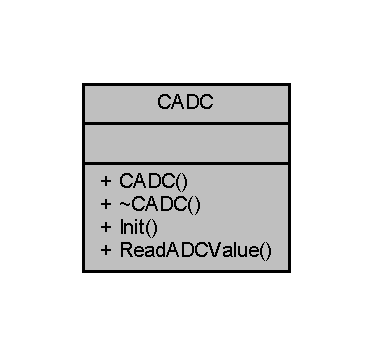
\includegraphics[width=179pt]{class_c_a_d_c__coll__graph}
\end{center}
\end{figure}
\subsection*{Public Member Functions}
\begin{DoxyCompactItemize}
\item 
\mbox{\hyperlink{class_c_a_d_c_aa312b17b94e31c72be8463a4a14838ec}{C\+A\+DC}} ()
\begin{DoxyCompactList}\small\item\em Constructor of \mbox{\hyperlink{class_c_a_d_c}{C\+A\+DC}}. \end{DoxyCompactList}\item 
\mbox{\hyperlink{class_c_a_d_c_ab8a5414ebb4c3707ac1575d63635efd8}{$\sim$\+C\+A\+DC}} ()
\begin{DoxyCompactList}\small\item\em Destructor of \mbox{\hyperlink{class_c_a_d_c}{C\+A\+DC}}. \end{DoxyCompactList}\item 
void \mbox{\hyperlink{class_c_a_d_c_a09118c55821cd6f0c9b2e2d2edd40d33}{Init}} ()
\begin{DoxyCompactList}\small\item\em Initialization function of \mbox{\hyperlink{class_c_a_d_c}{C\+A\+DC}}. \end{DoxyCompactList}\item 
\mbox{\hyperlink{_a_d_a_s___types_8h_a1f1825b69244eb3ad2c7165ddc99c956}{uint16\+\_\+t}} \mbox{\hyperlink{class_c_a_d_c_ac2f897fc64f605751ac3ffe7d2704ba6}{Read\+A\+D\+C\+Value}} (\mbox{\hyperlink{_a_d_a_s___types_8h_aba7bc1797add20fe3efdf37ced1182c5}{uint8\+\_\+t}} pin)
\begin{DoxyCompactList}\small\item\em Function to read A\+DC value. \end{DoxyCompactList}\end{DoxyCompactItemize}


\subsection{Detailed Description}
Hardware Abstraction Layer (H\+AL) A\+DC class. 

Definition at line 15 of file H\+A\+L\+\_\+\+A\+D\+C.\+h.



\subsection{Constructor \& Destructor Documentation}
\mbox{\Hypertarget{class_c_a_d_c_aa312b17b94e31c72be8463a4a14838ec}\label{class_c_a_d_c_aa312b17b94e31c72be8463a4a14838ec}} 
\index{CADC@{CADC}!CADC@{CADC}}
\index{CADC@{CADC}!CADC@{CADC}}
\subsubsection{\texorpdfstring{CADC()}{CADC()}}
{\footnotesize\ttfamily C\+A\+D\+C\+::\+C\+A\+DC (\begin{DoxyParamCaption}{ }\end{DoxyParamCaption})}



Constructor of \mbox{\hyperlink{class_c_a_d_c}{C\+A\+DC}}. 



Definition at line 13 of file H\+A\+L\+\_\+\+A\+D\+C.\+cpp.

\mbox{\Hypertarget{class_c_a_d_c_ab8a5414ebb4c3707ac1575d63635efd8}\label{class_c_a_d_c_ab8a5414ebb4c3707ac1575d63635efd8}} 
\index{CADC@{CADC}!````~CADC@{$\sim$CADC}}
\index{````~CADC@{$\sim$CADC}!CADC@{CADC}}
\subsubsection{\texorpdfstring{$\sim$CADC()}{~CADC()}}
{\footnotesize\ttfamily C\+A\+D\+C\+::$\sim$\+C\+A\+DC (\begin{DoxyParamCaption}{ }\end{DoxyParamCaption})}



Destructor of \mbox{\hyperlink{class_c_a_d_c}{C\+A\+DC}}. 



Definition at line 18 of file H\+A\+L\+\_\+\+A\+D\+C.\+cpp.



\subsection{Member Function Documentation}
\mbox{\Hypertarget{class_c_a_d_c_a09118c55821cd6f0c9b2e2d2edd40d33}\label{class_c_a_d_c_a09118c55821cd6f0c9b2e2d2edd40d33}} 
\index{CADC@{CADC}!Init@{Init}}
\index{Init@{Init}!CADC@{CADC}}
\subsubsection{\texorpdfstring{Init()}{Init()}}
{\footnotesize\ttfamily void C\+A\+D\+C\+::\+Init (\begin{DoxyParamCaption}\item[{void}]{ }\end{DoxyParamCaption})}



Initialization function of \mbox{\hyperlink{class_c_a_d_c}{C\+A\+DC}}. 



Definition at line 22 of file H\+A\+L\+\_\+\+A\+D\+C.\+cpp.

\mbox{\Hypertarget{class_c_a_d_c_ac2f897fc64f605751ac3ffe7d2704ba6}\label{class_c_a_d_c_ac2f897fc64f605751ac3ffe7d2704ba6}} 
\index{CADC@{CADC}!ReadADCValue@{ReadADCValue}}
\index{ReadADCValue@{ReadADCValue}!CADC@{CADC}}
\subsubsection{\texorpdfstring{ReadADCValue()}{ReadADCValue()}}
{\footnotesize\ttfamily \mbox{\hyperlink{_a_d_a_s___types_8h_a1f1825b69244eb3ad2c7165ddc99c956}{uint16\+\_\+t}} C\+A\+D\+C\+::\+Read\+A\+D\+C\+Value (\begin{DoxyParamCaption}\item[{\mbox{\hyperlink{_a_d_a_s___types_8h_aba7bc1797add20fe3efdf37ced1182c5}{uint8\+\_\+t}}}]{pin }\end{DoxyParamCaption})}



Function to read A\+DC value. 


\begin{DoxyParams}{Parameters}
{\em pin} & Pin number e.\+g. A0 \\
\hline
\end{DoxyParams}
\begin{DoxyReturn}{Returns}
Returns current A\+DC value 
\end{DoxyReturn}


Definition at line 30 of file H\+A\+L\+\_\+\+A\+D\+C.\+cpp.

Here is the caller graph for this function\+:\nopagebreak
\begin{figure}[H]
\begin{center}
\leavevmode
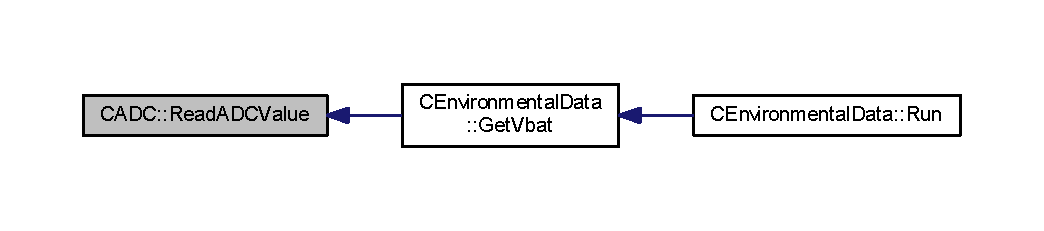
\includegraphics[width=350pt]{class_c_a_d_c_ac2f897fc64f605751ac3ffe7d2704ba6_icgraph}
\end{center}
\end{figure}


The documentation for this class was generated from the following files\+:\begin{DoxyCompactItemize}
\item 
\mbox{\hyperlink{_h_a_l___a_d_c_8h}{H\+A\+L\+\_\+\+A\+D\+C.\+h}}\item 
\mbox{\hyperlink{_h_a_l___a_d_c_8cpp}{H\+A\+L\+\_\+\+A\+D\+C.\+cpp}}\end{DoxyCompactItemize}

\hypertarget{class_c_buff_adas}{}\section{C\+Buff\+Adas Class Reference}
\label{class_c_buff_adas}\index{C\+Buff\+Adas@{C\+Buff\+Adas}}


{\ttfamily \#include $<$Cbuffer.\+h$>$}



Collaboration diagram for C\+Buff\+Adas\+:
\nopagebreak
\begin{figure}[H]
\begin{center}
\leavevmode
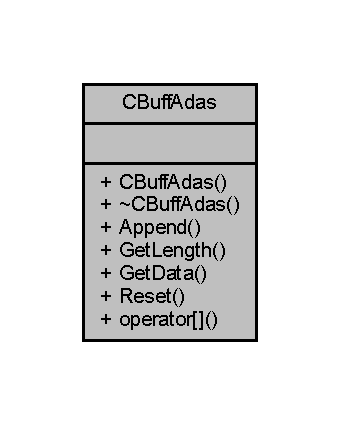
\includegraphics[width=163pt]{class_c_buff_adas__coll__graph}
\end{center}
\end{figure}
\subsection*{Public Member Functions}
\begin{DoxyCompactItemize}
\item 
\mbox{\hyperlink{class_c_buff_adas_a7491e123b003457b2565435ae7ac9ce4}{C\+Buff\+Adas}} (\mbox{\hyperlink{_a_d_a_s___types_8h_aba7bc1797add20fe3efdf37ced1182c5}{uint8\+\_\+t}} $\ast$data, const \mbox{\hyperlink{_a_d_a_s___types_8h_a1f1825b69244eb3ad2c7165ddc99c956}{uint16\+\_\+t}} len)
\begin{DoxyCompactList}\small\item\em Cbuffer constructor. \end{DoxyCompactList}\item 
\mbox{\hyperlink{class_c_buff_adas_a55af513577ba8522492fff4db85da247}{$\sim$\+C\+Buff\+Adas}} ()
\begin{DoxyCompactList}\small\item\em Cbuffer destructor. \end{DoxyCompactList}\item 
void \mbox{\hyperlink{class_c_buff_adas_aceac4b71872e406861286959f578c89b}{Append}} (const \mbox{\hyperlink{_a_d_a_s___types_8h_aba7bc1797add20fe3efdf37ced1182c5}{uint8\+\_\+t}} data)
\begin{DoxyCompactList}\small\item\em Append data. \end{DoxyCompactList}\item 
\mbox{\hyperlink{_a_d_a_s___types_8h_a1f1825b69244eb3ad2c7165ddc99c956}{uint16\+\_\+t}} \mbox{\hyperlink{class_c_buff_adas_a493f61488df8ac9f7e942af1a2fbdbf3}{Get\+Length}} ()
\begin{DoxyCompactList}\small\item\em get lenght \end{DoxyCompactList}\item 
\mbox{\hyperlink{_a_d_a_s___types_8h_aba7bc1797add20fe3efdf37ced1182c5}{uint8\+\_\+t}} $\ast$ \mbox{\hyperlink{class_c_buff_adas_a56fdcdc9766874d3a6fef04119ee91f9}{Get\+Data}} ()
\begin{DoxyCompactList}\small\item\em get buffer pointer \end{DoxyCompactList}\item 
void \mbox{\hyperlink{class_c_buff_adas_a2ff1ee5f1dfa56117d76b17027d7b7e8}{Reset}} ()
\begin{DoxyCompactList}\small\item\em reset buffer \end{DoxyCompactList}\item 
\mbox{\hyperlink{_a_d_a_s___types_8h_a06896e8c53f721507066c079052171f8}{uint32\+\_\+t}} \mbox{\hyperlink{class_c_buff_adas_ae1a6aa5f049b0e1e04950af1c55df3d7}{operator\mbox{[}$\,$\mbox{]}}} (const \mbox{\hyperlink{_a_d_a_s___types_8h_a06896e8c53f721507066c079052171f8}{uint32\+\_\+t}} index)
\begin{DoxyCompactList}\small\item\em operator overloading \mbox{[}\mbox{]} \end{DoxyCompactList}\end{DoxyCompactItemize}


\subsection{Detailed Description}


Definition at line 13 of file Cbuffer.\+h.



\subsection{Constructor \& Destructor Documentation}
\mbox{\Hypertarget{class_c_buff_adas_a7491e123b003457b2565435ae7ac9ce4}\label{class_c_buff_adas_a7491e123b003457b2565435ae7ac9ce4}} 
\index{C\+Buff\+Adas@{C\+Buff\+Adas}!C\+Buff\+Adas@{C\+Buff\+Adas}}
\index{C\+Buff\+Adas@{C\+Buff\+Adas}!C\+Buff\+Adas@{C\+Buff\+Adas}}
\subsubsection{\texorpdfstring{C\+Buff\+Adas()}{CBuffAdas()}}
{\footnotesize\ttfamily C\+Buff\+Adas\+::\+C\+Buff\+Adas (\begin{DoxyParamCaption}\item[{\mbox{\hyperlink{_a_d_a_s___types_8h_aba7bc1797add20fe3efdf37ced1182c5}{uint8\+\_\+t}} $\ast$}]{data,  }\item[{const \mbox{\hyperlink{_a_d_a_s___types_8h_a1f1825b69244eb3ad2c7165ddc99c956}{uint16\+\_\+t}}}]{len }\end{DoxyParamCaption})}



Cbuffer constructor. 

Instantiation and initialization 
\begin{DoxyParams}[1]{Parameters}
\mbox{\tt in}  & {\em data} & buffer memory pointer \\
\hline
\mbox{\tt in}  & {\em len} & length of buffer memory \\
\hline
\end{DoxyParams}


Definition at line 4 of file Cbuffer.\+cpp.

\mbox{\Hypertarget{class_c_buff_adas_a55af513577ba8522492fff4db85da247}\label{class_c_buff_adas_a55af513577ba8522492fff4db85da247}} 
\index{C\+Buff\+Adas@{C\+Buff\+Adas}!````~C\+Buff\+Adas@{$\sim$\+C\+Buff\+Adas}}
\index{````~C\+Buff\+Adas@{$\sim$\+C\+Buff\+Adas}!C\+Buff\+Adas@{C\+Buff\+Adas}}
\subsubsection{\texorpdfstring{$\sim$\+C\+Buff\+Adas()}{~CBuffAdas()}}
{\footnotesize\ttfamily C\+Buff\+Adas\+::$\sim$\+C\+Buff\+Adas (\begin{DoxyParamCaption}{ }\end{DoxyParamCaption})}



Cbuffer destructor. 



Definition at line 12 of file Cbuffer.\+cpp.



\subsection{Member Function Documentation}
\mbox{\Hypertarget{class_c_buff_adas_aceac4b71872e406861286959f578c89b}\label{class_c_buff_adas_aceac4b71872e406861286959f578c89b}} 
\index{C\+Buff\+Adas@{C\+Buff\+Adas}!Append@{Append}}
\index{Append@{Append}!C\+Buff\+Adas@{C\+Buff\+Adas}}
\subsubsection{\texorpdfstring{Append()}{Append()}}
{\footnotesize\ttfamily void C\+Buff\+Adas\+::\+Append (\begin{DoxyParamCaption}\item[{const \mbox{\hyperlink{_a_d_a_s___types_8h_aba7bc1797add20fe3efdf37ced1182c5}{uint8\+\_\+t}}}]{data }\end{DoxyParamCaption})}



Append data. 


\begin{DoxyParams}[1]{Parameters}
\mbox{\tt in}  & {\em data} & byte to be appended \\
\hline
\end{DoxyParams}


Definition at line 18 of file Cbuffer.\+cpp.

\mbox{\Hypertarget{class_c_buff_adas_a56fdcdc9766874d3a6fef04119ee91f9}\label{class_c_buff_adas_a56fdcdc9766874d3a6fef04119ee91f9}} 
\index{C\+Buff\+Adas@{C\+Buff\+Adas}!Get\+Data@{Get\+Data}}
\index{Get\+Data@{Get\+Data}!C\+Buff\+Adas@{C\+Buff\+Adas}}
\subsubsection{\texorpdfstring{Get\+Data()}{GetData()}}
{\footnotesize\ttfamily \mbox{\hyperlink{_a_d_a_s___types_8h_aba7bc1797add20fe3efdf37ced1182c5}{uint8\+\_\+t}} $\ast$ C\+Buff\+Adas\+::\+Get\+Data (\begin{DoxyParamCaption}{ }\end{DoxyParamCaption})}



get buffer pointer 

\begin{DoxyReturn}{Returns}
pointer to buffer 
\end{DoxyReturn}


Definition at line 31 of file Cbuffer.\+cpp.

\mbox{\Hypertarget{class_c_buff_adas_a493f61488df8ac9f7e942af1a2fbdbf3}\label{class_c_buff_adas_a493f61488df8ac9f7e942af1a2fbdbf3}} 
\index{C\+Buff\+Adas@{C\+Buff\+Adas}!Get\+Length@{Get\+Length}}
\index{Get\+Length@{Get\+Length}!C\+Buff\+Adas@{C\+Buff\+Adas}}
\subsubsection{\texorpdfstring{Get\+Length()}{GetLength()}}
{\footnotesize\ttfamily \mbox{\hyperlink{_a_d_a_s___types_8h_a1f1825b69244eb3ad2c7165ddc99c956}{uint16\+\_\+t}} C\+Buff\+Adas\+::\+Get\+Length (\begin{DoxyParamCaption}{ }\end{DoxyParamCaption})}



get lenght 

\begin{DoxyReturn}{Returns}
length of used buffer 
\end{DoxyReturn}


Definition at line 26 of file Cbuffer.\+cpp.

\mbox{\Hypertarget{class_c_buff_adas_ae1a6aa5f049b0e1e04950af1c55df3d7}\label{class_c_buff_adas_ae1a6aa5f049b0e1e04950af1c55df3d7}} 
\index{C\+Buff\+Adas@{C\+Buff\+Adas}!operator\mbox{[}\mbox{]}@{operator[]}}
\index{operator\mbox{[}\mbox{]}@{operator[]}!C\+Buff\+Adas@{C\+Buff\+Adas}}
\subsubsection{\texorpdfstring{operator[]()}{operator[]()}}
{\footnotesize\ttfamily \mbox{\hyperlink{_a_d_a_s___types_8h_a06896e8c53f721507066c079052171f8}{uint32\+\_\+t}} C\+Buff\+Adas\+::operator\mbox{[}$\,$\mbox{]} (\begin{DoxyParamCaption}\item[{const \mbox{\hyperlink{_a_d_a_s___types_8h_a06896e8c53f721507066c079052171f8}{uint32\+\_\+t}}}]{index }\end{DoxyParamCaption})}



operator overloading \mbox{[}\mbox{]} 


\begin{DoxyParams}{Parameters}
{\em index} & index \\
\hline
\end{DoxyParams}
\begin{DoxyReturn}{Returns}
uint32\+\_\+t 
\end{DoxyReturn}


Definition at line 41 of file Cbuffer.\+cpp.

\mbox{\Hypertarget{class_c_buff_adas_a2ff1ee5f1dfa56117d76b17027d7b7e8}\label{class_c_buff_adas_a2ff1ee5f1dfa56117d76b17027d7b7e8}} 
\index{C\+Buff\+Adas@{C\+Buff\+Adas}!Reset@{Reset}}
\index{Reset@{Reset}!C\+Buff\+Adas@{C\+Buff\+Adas}}
\subsubsection{\texorpdfstring{Reset()}{Reset()}}
{\footnotesize\ttfamily void C\+Buff\+Adas\+::\+Reset (\begin{DoxyParamCaption}{ }\end{DoxyParamCaption})}



reset buffer 



Definition at line 36 of file Cbuffer.\+cpp.

Here is the caller graph for this function\+:
\nopagebreak
\begin{figure}[H]
\begin{center}
\leavevmode
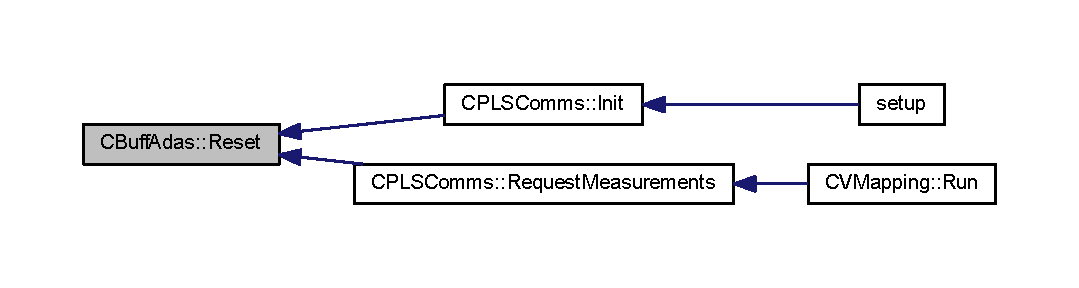
\includegraphics[width=350pt]{class_c_buff_adas_a2ff1ee5f1dfa56117d76b17027d7b7e8_icgraph}
\end{center}
\end{figure}


The documentation for this class was generated from the following files\+:\begin{DoxyCompactItemize}
\item 
\mbox{\hyperlink{_cbuffer_8h}{Cbuffer.\+h}}\item 
\mbox{\hyperlink{_cbuffer_8cpp}{Cbuffer.\+cpp}}\end{DoxyCompactItemize}

\hypertarget{class_c_environmental_data}{}\section{C\+Environmental\+Data Class Reference}
\label{class_c_environmental_data}\index{C\+Environmental\+Data@{C\+Environmental\+Data}}


Environmental Data Class.  




{\ttfamily \#include $<$App\+\_\+\+Environmental\+Data.\+h$>$}



Inheritance diagram for C\+Environmental\+Data\+:\nopagebreak
\begin{figure}[H]
\begin{center}
\leavevmode
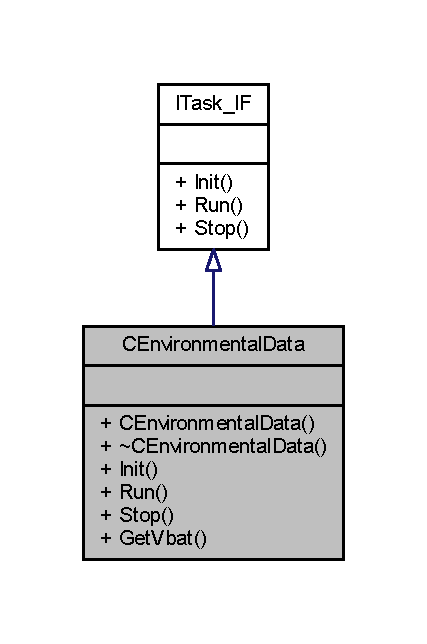
\includegraphics[width=205pt]{class_c_environmental_data__inherit__graph}
\end{center}
\end{figure}


Collaboration diagram for C\+Environmental\+Data\+:\nopagebreak
\begin{figure}[H]
\begin{center}
\leavevmode
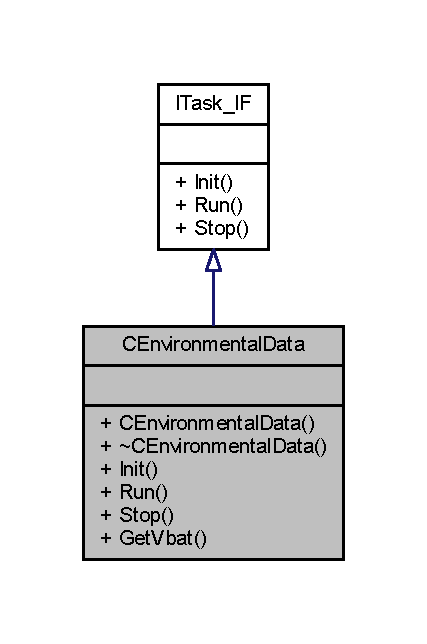
\includegraphics[width=205pt]{class_c_environmental_data__coll__graph}
\end{center}
\end{figure}
\subsection*{Public Member Functions}
\begin{DoxyCompactItemize}
\item 
\mbox{\hyperlink{class_c_environmental_data_a93b5c52fc18b109c6f1de9d3a5007033}{C\+Environmental\+Data}} ()
\begin{DoxyCompactList}\small\item\em Constructor of \mbox{\hyperlink{class_c_environmental_data}{C\+Environmental\+Data}}. \end{DoxyCompactList}\item 
\mbox{\hyperlink{class_c_environmental_data_a9ec6952d01bbc0b5813889237535b71d}{$\sim$\+C\+Environmental\+Data}} ()
\begin{DoxyCompactList}\small\item\em Destructor of \mbox{\hyperlink{class_c_environmental_data}{C\+Environmental\+Data}}. \end{DoxyCompactList}\item 
virtual void \mbox{\hyperlink{class_c_environmental_data_a3321cce122ef1e1f7e995ee51353e87d}{Init}} (void)
\begin{DoxyCompactList}\small\item\em Initialization function of \mbox{\hyperlink{class_c_environmental_data}{C\+Environmental\+Data}}. \end{DoxyCompactList}\item 
virtual void \mbox{\hyperlink{class_c_environmental_data_a586a729d3aab2873812517d950c91242}{Run}} (void)
\begin{DoxyCompactList}\small\item\em Run function of \mbox{\hyperlink{class_c_environmental_data}{C\+Environmental\+Data}} which is periodically called by \mbox{\hyperlink{class_c_task_ctrl}{C\+Task\+Ctrl}}. \end{DoxyCompactList}\item 
virtual void \mbox{\hyperlink{class_c_environmental_data_a61a8f487f013602aab4dadcf8a9da4c8}{Stop}} (void)
\begin{DoxyCompactList}\small\item\em Stop function of \mbox{\hyperlink{class_c_environmental_data}{C\+Environmental\+Data}}. \end{DoxyCompactList}\item 
virtual \mbox{\hyperlink{_a_d_a_s___types_8h_a1f1825b69244eb3ad2c7165ddc99c956}{uint16\+\_\+t}} \mbox{\hyperlink{class_c_environmental_data_a12a6d60a2a0aa406beb82375fa60e875}{Get\+Vbat}} (void)
\begin{DoxyCompactList}\small\item\em Function to convert A\+DC value into mV. \end{DoxyCompactList}\end{DoxyCompactItemize}


\subsection{Detailed Description}
Environmental Data Class. 

Definition at line 19 of file App\+\_\+\+Environmental\+Data.\+h.



\subsection{Constructor \& Destructor Documentation}
\mbox{\Hypertarget{class_c_environmental_data_a93b5c52fc18b109c6f1de9d3a5007033}\label{class_c_environmental_data_a93b5c52fc18b109c6f1de9d3a5007033}} 
\index{C\+Environmental\+Data@{C\+Environmental\+Data}!C\+Environmental\+Data@{C\+Environmental\+Data}}
\index{C\+Environmental\+Data@{C\+Environmental\+Data}!C\+Environmental\+Data@{C\+Environmental\+Data}}
\subsubsection{\texorpdfstring{C\+Environmental\+Data()}{CEnvironmentalData()}}
{\footnotesize\ttfamily C\+Environmental\+Data\+::\+C\+Environmental\+Data (\begin{DoxyParamCaption}{ }\end{DoxyParamCaption})}



Constructor of \mbox{\hyperlink{class_c_environmental_data}{C\+Environmental\+Data}}. 



Definition at line 13 of file App\+\_\+\+Environmental\+Data.\+cpp.

\mbox{\Hypertarget{class_c_environmental_data_a9ec6952d01bbc0b5813889237535b71d}\label{class_c_environmental_data_a9ec6952d01bbc0b5813889237535b71d}} 
\index{C\+Environmental\+Data@{C\+Environmental\+Data}!````~C\+Environmental\+Data@{$\sim$\+C\+Environmental\+Data}}
\index{````~C\+Environmental\+Data@{$\sim$\+C\+Environmental\+Data}!C\+Environmental\+Data@{C\+Environmental\+Data}}
\subsubsection{\texorpdfstring{$\sim$\+C\+Environmental\+Data()}{~CEnvironmentalData()}}
{\footnotesize\ttfamily C\+Environmental\+Data\+::$\sim$\+C\+Environmental\+Data (\begin{DoxyParamCaption}{ }\end{DoxyParamCaption})}



Destructor of \mbox{\hyperlink{class_c_environmental_data}{C\+Environmental\+Data}}. 



Definition at line 18 of file App\+\_\+\+Environmental\+Data.\+cpp.



\subsection{Member Function Documentation}
\mbox{\Hypertarget{class_c_environmental_data_a12a6d60a2a0aa406beb82375fa60e875}\label{class_c_environmental_data_a12a6d60a2a0aa406beb82375fa60e875}} 
\index{C\+Environmental\+Data@{C\+Environmental\+Data}!Get\+Vbat@{Get\+Vbat}}
\index{Get\+Vbat@{Get\+Vbat}!C\+Environmental\+Data@{C\+Environmental\+Data}}
\subsubsection{\texorpdfstring{Get\+Vbat()}{GetVbat()}}
{\footnotesize\ttfamily \mbox{\hyperlink{_a_d_a_s___types_8h_a1f1825b69244eb3ad2c7165ddc99c956}{uint16\+\_\+t}} C\+Environmental\+Data\+::\+Get\+Vbat (\begin{DoxyParamCaption}\item[{void}]{ }\end{DoxyParamCaption})\hspace{0.3cm}{\ttfamily [virtual]}}



Function to convert A\+DC value into mV. 

The analog input pin has to defined at \mbox{\hyperlink{_a_d_a_s___cfg_8h_ad9c869803f9fc9e3ffc9e962c19f028d}{P\+I\+N\+\_\+\+V\+B\+AT}}. \begin{DoxyReturn}{Returns}
Returns the battery voltage in mV according to the parameters \mbox{\hyperlink{_a_d_a_s___cfg_8h_a9b007d258cc627ea79aa06cef42c0851}{E\+N\+V\+\_\+\+V\+B\+A\+T\+\_\+\+G\+A\+IN}} and \mbox{\hyperlink{_a_d_a_s___cfg_8h_a60f7517e6d36bf5703fc24eacb2f17ed}{E\+N\+V\+\_\+\+V\+B\+A\+T\+\_\+\+O\+FF}} 
\end{DoxyReturn}


Definition at line 61 of file App\+\_\+\+Environmental\+Data.\+cpp.

Here is the call graph for this function\+:\nopagebreak
\begin{figure}[H]
\begin{center}
\leavevmode
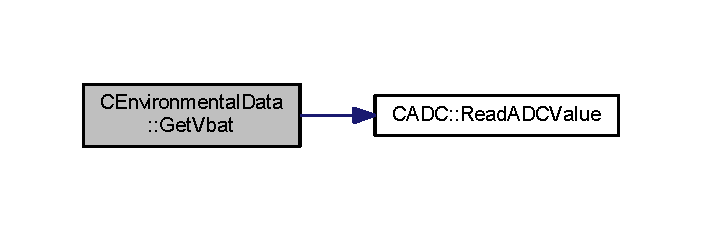
\includegraphics[width=337pt]{class_c_environmental_data_a12a6d60a2a0aa406beb82375fa60e875_cgraph}
\end{center}
\end{figure}
Here is the caller graph for this function\+:\nopagebreak
\begin{figure}[H]
\begin{center}
\leavevmode
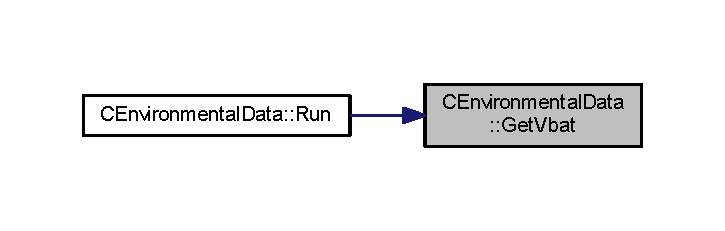
\includegraphics[width=348pt]{class_c_environmental_data_a12a6d60a2a0aa406beb82375fa60e875_icgraph}
\end{center}
\end{figure}
\mbox{\Hypertarget{class_c_environmental_data_a3321cce122ef1e1f7e995ee51353e87d}\label{class_c_environmental_data_a3321cce122ef1e1f7e995ee51353e87d}} 
\index{C\+Environmental\+Data@{C\+Environmental\+Data}!Init@{Init}}
\index{Init@{Init}!C\+Environmental\+Data@{C\+Environmental\+Data}}
\subsubsection{\texorpdfstring{Init()}{Init()}}
{\footnotesize\ttfamily void C\+Environmental\+Data\+::\+Init (\begin{DoxyParamCaption}\item[{void}]{ }\end{DoxyParamCaption})\hspace{0.3cm}{\ttfamily [virtual]}}



Initialization function of \mbox{\hyperlink{class_c_environmental_data}{C\+Environmental\+Data}}. 



Implements \mbox{\hyperlink{class_i_task___i_f_a28f608bdb9b19658403f7b9b7421968d}{I\+Task\+\_\+\+IF}}.



Definition at line 23 of file App\+\_\+\+Environmental\+Data.\+cpp.

\mbox{\Hypertarget{class_c_environmental_data_a586a729d3aab2873812517d950c91242}\label{class_c_environmental_data_a586a729d3aab2873812517d950c91242}} 
\index{C\+Environmental\+Data@{C\+Environmental\+Data}!Run@{Run}}
\index{Run@{Run}!C\+Environmental\+Data@{C\+Environmental\+Data}}
\subsubsection{\texorpdfstring{Run()}{Run()}}
{\footnotesize\ttfamily void C\+Environmental\+Data\+::\+Run (\begin{DoxyParamCaption}\item[{void}]{ }\end{DoxyParamCaption})\hspace{0.3cm}{\ttfamily [virtual]}}



Run function of \mbox{\hyperlink{class_c_environmental_data}{C\+Environmental\+Data}} which is periodically called by \mbox{\hyperlink{class_c_task_ctrl}{C\+Task\+Ctrl}}. 

Function reads battery voltage and prints warning message on serial interface 

Implements \mbox{\hyperlink{class_i_task___i_f_ab73cc5879a61d00fc59b72cce32cc6f7}{I\+Task\+\_\+\+IF}}.



Definition at line 32 of file App\+\_\+\+Environmental\+Data.\+cpp.

Here is the call graph for this function\+:\nopagebreak
\begin{figure}[H]
\begin{center}
\leavevmode
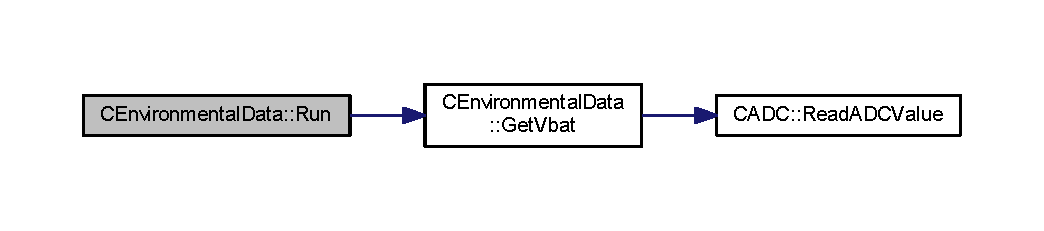
\includegraphics[width=350pt]{class_c_environmental_data_a586a729d3aab2873812517d950c91242_cgraph}
\end{center}
\end{figure}
\mbox{\Hypertarget{class_c_environmental_data_a61a8f487f013602aab4dadcf8a9da4c8}\label{class_c_environmental_data_a61a8f487f013602aab4dadcf8a9da4c8}} 
\index{C\+Environmental\+Data@{C\+Environmental\+Data}!Stop@{Stop}}
\index{Stop@{Stop}!C\+Environmental\+Data@{C\+Environmental\+Data}}
\subsubsection{\texorpdfstring{Stop()}{Stop()}}
{\footnotesize\ttfamily void C\+Environmental\+Data\+::\+Stop (\begin{DoxyParamCaption}\item[{void}]{ }\end{DoxyParamCaption})\hspace{0.3cm}{\ttfamily [virtual]}}



Stop function of \mbox{\hyperlink{class_c_environmental_data}{C\+Environmental\+Data}}. 



Implements \mbox{\hyperlink{class_i_task___i_f_af5f8fba86704c7e36d0e4681d58300c6}{I\+Task\+\_\+\+IF}}.



Definition at line 51 of file App\+\_\+\+Environmental\+Data.\+cpp.



The documentation for this class was generated from the following files\+:\begin{DoxyCompactItemize}
\item 
\mbox{\hyperlink{_app___environmental_data_8h}{App\+\_\+\+Environmental\+Data.\+h}}\item 
\mbox{\hyperlink{_app___environmental_data_8cpp}{App\+\_\+\+Environmental\+Data.\+cpp}}\end{DoxyCompactItemize}

\hypertarget{class_c_i_c_c_comms}{}\section{C\+I\+C\+C\+Comms Class Reference}
\label{class_c_i_c_c_comms}\index{CICCComms@{CICCComms}}


{\ttfamily \#include $<$Comm\+\_\+\+I\+C\+C.\+h$>$}



Collaboration diagram for C\+I\+C\+C\+Comms\+:
% FIG 0
\subsection*{Classes}
\begin{DoxyCompactItemize}
\item 
struct \mbox{\hyperlink{struct_c_i_c_c_comms_1_1_message__t}{Message\+\_\+t}}
\end{DoxyCompactItemize}
\subsection*{Public Member Functions}
\begin{DoxyCompactItemize}
\item 
\mbox{\hyperlink{class_c_i_c_c_comms_af2cb9bb6ab473bc5ea2b4aa2f98084ff}{C\+I\+C\+C\+Comms}} (\mbox{\hyperlink{class_c_serial}{C\+Serial}} \&ser\+Port)
\item 
\mbox{\hyperlink{class_c_i_c_c_comms_a951ae11fd2024309bd4ecf67981287e7}{$\sim$\+C\+I\+C\+C\+Comms}} ()
\item 
virtual void \mbox{\hyperlink{class_c_i_c_c_comms_a56fc0858965ed1f1f9b3295602472c7e}{Init}} (\mbox{\hyperlink{class_c_motor_ctrl}{C\+Motor\+Ctrl}} $\ast$\mbox{\hyperlink{_a_d_a_s___m_c_u_8ino_ab618fa643b3224c905b4fcbd074fb481}{m\+Ctrl\+\_\+o}})
\item 
virtual void \mbox{\hyperlink{class_c_i_c_c_comms_a8b3fa81307b3b9ba0e72b4aee8279c56}{Run}} (void)
\item 
virtual void \mbox{\hyperlink{class_c_i_c_c_comms_ab925dd7ff82f30ccd9f770ab2281b3ab}{add\+Tx\+Msg}} (\mbox{\hyperlink{_a_d_a_s___types_8h_aba7bc1797add20fe3efdf37ced1182c5}{uint8\+\_\+t}} cmd, signed int data)
\end{DoxyCompactItemize}
\subsection*{Public Attributes}
\begin{DoxyCompactItemize}
\item 
\mbox{\hyperlink{struct_c_i_c_c_comms_1_1_message__t}{Message\+\_\+t}} \mbox{\hyperlink{class_c_i_c_c_comms_a35a59d11110d830b70ab5e2a5644bbb9}{msg}}
\end{DoxyCompactItemize}


\subsection{Detailed Description}


Definition at line 17 of file Comm\+\_\+\+I\+C\+C.\+h.



\subsection{Constructor \& Destructor Documentation}
\mbox{\Hypertarget{class_c_i_c_c_comms_af2cb9bb6ab473bc5ea2b4aa2f98084ff}\label{class_c_i_c_c_comms_af2cb9bb6ab473bc5ea2b4aa2f98084ff}} 
\index{CICCComms@{CICCComms}!CICCComms@{CICCComms}}
\index{CICCComms@{CICCComms}!CICCComms@{CICCComms}}
\subsubsection{\texorpdfstring{CICCComms()}{CICCComms()}}
{\footnotesize\ttfamily C\+I\+C\+C\+Comms\+::\+C\+I\+C\+C\+Comms (\begin{DoxyParamCaption}\item[{\mbox{\hyperlink{class_c_serial}{C\+Serial}} \&}]{ser\+Port }\end{DoxyParamCaption})}



Definition at line 6 of file Comm\+\_\+\+I\+C\+C.\+cpp.

\mbox{\Hypertarget{class_c_i_c_c_comms_a951ae11fd2024309bd4ecf67981287e7}\label{class_c_i_c_c_comms_a951ae11fd2024309bd4ecf67981287e7}} 
\index{CICCComms@{CICCComms}!````~CICCComms@{$\sim$CICCComms}}
\index{````~CICCComms@{$\sim$CICCComms}!CICCComms@{CICCComms}}
\subsubsection{\texorpdfstring{$\sim$CICCComms()}{~CICCComms()}}
{\footnotesize\ttfamily C\+I\+C\+C\+Comms\+::$\sim$\+C\+I\+C\+C\+Comms (\begin{DoxyParamCaption}{ }\end{DoxyParamCaption})}



Definition at line 11 of file Comm\+\_\+\+I\+C\+C.\+cpp.



\subsection{Member Function Documentation}
\mbox{\Hypertarget{class_c_i_c_c_comms_ab925dd7ff82f30ccd9f770ab2281b3ab}\label{class_c_i_c_c_comms_ab925dd7ff82f30ccd9f770ab2281b3ab}} 
\index{CICCComms@{CICCComms}!addTxMsg@{addTxMsg}}
\index{addTxMsg@{addTxMsg}!CICCComms@{CICCComms}}
\subsubsection{\texorpdfstring{addTxMsg()}{addTxMsg()}}
{\footnotesize\ttfamily void C\+I\+C\+C\+Comms\+::add\+Tx\+Msg (\begin{DoxyParamCaption}\item[{\mbox{\hyperlink{_a_d_a_s___types_8h_aba7bc1797add20fe3efdf37ced1182c5}{uint8\+\_\+t}}}]{cmd,  }\item[{signed int}]{data }\end{DoxyParamCaption})\hspace{0.3cm}{\ttfamily [virtual]}}



Definition at line 107 of file Comm\+\_\+\+I\+C\+C.\+cpp.

\mbox{\Hypertarget{class_c_i_c_c_comms_a56fc0858965ed1f1f9b3295602472c7e}\label{class_c_i_c_c_comms_a56fc0858965ed1f1f9b3295602472c7e}} 
\index{CICCComms@{CICCComms}!Init@{Init}}
\index{Init@{Init}!CICCComms@{CICCComms}}
\subsubsection{\texorpdfstring{Init()}{Init()}}
{\footnotesize\ttfamily void C\+I\+C\+C\+Comms\+::\+Init (\begin{DoxyParamCaption}\item[{\mbox{\hyperlink{class_c_motor_ctrl}{C\+Motor\+Ctrl}} $\ast$}]{m\+Ctrl\+\_\+o }\end{DoxyParamCaption})\hspace{0.3cm}{\ttfamily [virtual]}}



Definition at line 16 of file Comm\+\_\+\+I\+C\+C.\+cpp.

Here is the caller graph for this function\+:
% FIG 1
\mbox{\Hypertarget{class_c_i_c_c_comms_a8b3fa81307b3b9ba0e72b4aee8279c56}\label{class_c_i_c_c_comms_a8b3fa81307b3b9ba0e72b4aee8279c56}} 
\index{CICCComms@{CICCComms}!Run@{Run}}
\index{Run@{Run}!CICCComms@{CICCComms}}
\subsubsection{\texorpdfstring{Run()}{Run()}}
{\footnotesize\ttfamily void C\+I\+C\+C\+Comms\+::\+Run (\begin{DoxyParamCaption}\item[{void}]{ }\end{DoxyParamCaption})\hspace{0.3cm}{\ttfamily [virtual]}}



Definition at line 21 of file Comm\+\_\+\+I\+C\+C.\+cpp.

Here is the call graph for this function\+:
% FIG 2
Here is the caller graph for this function\+:
% FIG 3


\subsection{Member Data Documentation}
\mbox{\Hypertarget{class_c_i_c_c_comms_a35a59d11110d830b70ab5e2a5644bbb9}\label{class_c_i_c_c_comms_a35a59d11110d830b70ab5e2a5644bbb9}} 
\index{CICCComms@{CICCComms}!msg@{msg}}
\index{msg@{msg}!CICCComms@{CICCComms}}
\subsubsection{\texorpdfstring{msg}{msg}}
{\footnotesize\ttfamily \mbox{\hyperlink{struct_c_i_c_c_comms_1_1_message__t}{Message\+\_\+t}} C\+I\+C\+C\+Comms\+::msg}



Definition at line 45 of file Comm\+\_\+\+I\+C\+C.\+h.



The documentation for this class was generated from the following files\+:\begin{DoxyCompactItemize}
\item 
\mbox{\hyperlink{_comm___i_c_c_8h}{Comm\+\_\+\+I\+C\+C.\+h}}\item 
\mbox{\hyperlink{_comm___i_c_c_8cpp}{Comm\+\_\+\+I\+C\+C.\+cpp}}\end{DoxyCompactItemize}

\hypertarget{class_c_navigation}{}\section{C\+Navigation Class Reference}
\label{class_c_navigation}\index{C\+Navigation@{C\+Navigation}}


Navigation algorithm class.  




{\ttfamily \#include $<$App\+\_\+\+Navigation.\+h$>$}



Inheritance diagram for C\+Navigation\+:
\nopagebreak
\begin{figure}[H]
\begin{center}
\leavevmode
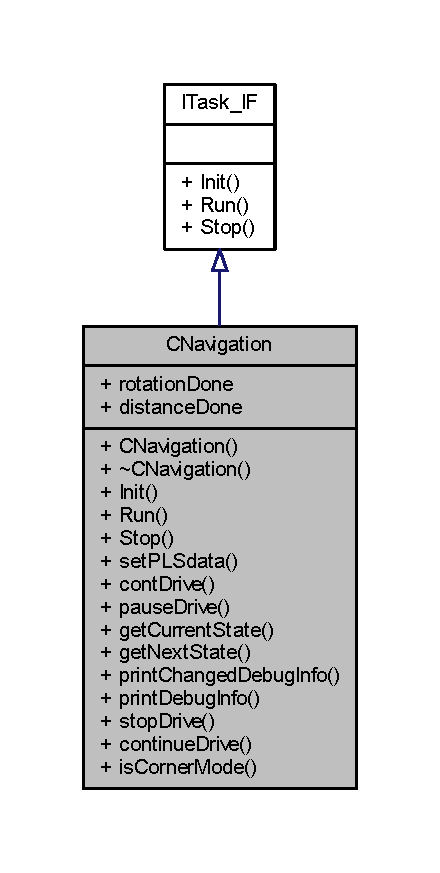
\includegraphics[width=211pt]{class_c_navigation__inherit__graph}
\end{center}
\end{figure}


Collaboration diagram for C\+Navigation\+:
\nopagebreak
\begin{figure}[H]
\begin{center}
\leavevmode
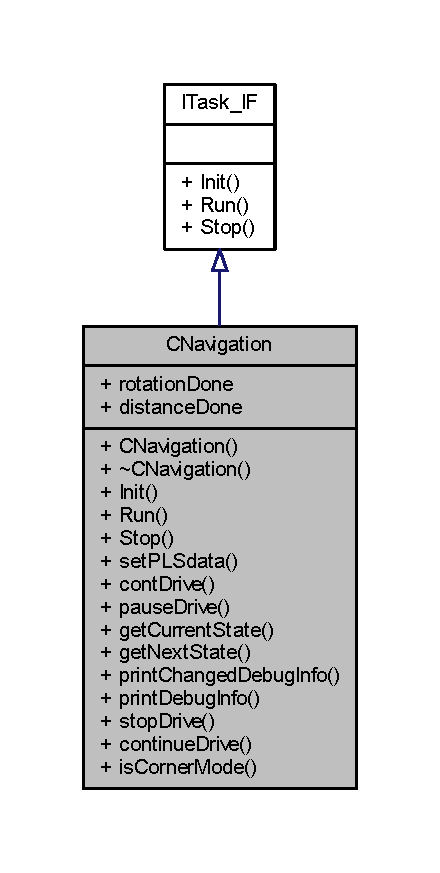
\includegraphics[width=211pt]{class_c_navigation__coll__graph}
\end{center}
\end{figure}
\subsection*{Public Types}
\begin{DoxyCompactItemize}
\item 
enum \mbox{\hyperlink{class_c_navigation_add9fc966c7604990edf5c2a2e0eba32c}{N\+A\+V\+\_\+\+S\+T\+A\+TE}} \{ \newline
\mbox{\hyperlink{class_c_navigation_add9fc966c7604990edf5c2a2e0eba32cad43f30d3a76f0217001df58807ce35e4}{S\+T\+A\+T\+E\+\_\+\+I\+D\+LE}}, 
\mbox{\hyperlink{class_c_navigation_add9fc966c7604990edf5c2a2e0eba32caed2dba9e927059d4fc3558e70dc9600d}{S\+T\+A\+T\+E\+\_\+\+G\+E\+T\+\_\+\+O\+F\+F\+S\+ET}}, 
\mbox{\hyperlink{class_c_navigation_add9fc966c7604990edf5c2a2e0eba32ca98c3278af5b38d612158bf91e361666b}{S\+T\+A\+T\+E\+\_\+\+R\+O\+T\+\_\+\+W\+A\+L\+L\+\_\+\+I\+N\+F\+R\+O\+NT}}, 
\mbox{\hyperlink{class_c_navigation_add9fc966c7604990edf5c2a2e0eba32ca499b515432a6f3518ffdc0042e6a0d0a}{S\+T\+A\+T\+E\+\_\+\+C\+O\+R\+\_\+\+O\+F\+F\+S\+ET}}, 
\newline
\mbox{\hyperlink{class_c_navigation_add9fc966c7604990edf5c2a2e0eba32cacaa28abfeaa777af95ae7de6c56c2f70}{S\+T\+A\+T\+E\+\_\+\+R\+O\+T\+\_\+\+W\+A\+L\+L\+\_\+\+O\+F\+F\+S\+ET}}, 
\mbox{\hyperlink{class_c_navigation_add9fc966c7604990edf5c2a2e0eba32caec4a96c2bd42d64f06d1d9ff729439f3}{S\+T\+A\+T\+E\+\_\+\+G\+E\+T\+\_\+\+A\+N\+G\+LE}}, 
\mbox{\hyperlink{class_c_navigation_add9fc966c7604990edf5c2a2e0eba32caf62bf4e18725aec5f8dcdb0b28ffad23}{S\+T\+A\+T\+E\+\_\+\+R\+O\+T\+\_\+\+W\+A\+LL}}, 
\mbox{\hyperlink{class_c_navigation_add9fc966c7604990edf5c2a2e0eba32caf1c06acfa5b7fed4fa82ed8ab9c42d10}{S\+T\+A\+T\+E\+\_\+\+D\+R\+I\+V\+E\+\_\+\+W\+A\+LL}}
 \}
\begin{DoxyCompactList}\small\item\em States of navigation flow. \end{DoxyCompactList}\end{DoxyCompactItemize}
\subsection*{Public Member Functions}
\begin{DoxyCompactItemize}
\item 
\mbox{\hyperlink{class_c_navigation_a0527efabaf4644c8c4e7910efec36e82}{C\+Navigation}} (\mbox{\hyperlink{class_c_i_c_c_comms}{C\+I\+C\+C\+Comms}} \&I\+CC)
\begin{DoxyCompactList}\small\item\em Constructor of \mbox{\hyperlink{class_c_navigation}{C\+Navigation}}. \end{DoxyCompactList}\item 
\mbox{\hyperlink{class_c_navigation_ae4c7c3e27ded45a94bc268634a7739da}{$\sim$\+C\+Navigation}} ()
\begin{DoxyCompactList}\small\item\em Destructor of \mbox{\hyperlink{class_c_navigation}{C\+Navigation}}. \end{DoxyCompactList}\item 
virtual void \mbox{\hyperlink{class_c_navigation_a86a0756663ccf76e9c474764b8f7a04f}{Init}} (void)
\begin{DoxyCompactList}\small\item\em Initialization function of \mbox{\hyperlink{class_c_navigation}{C\+Navigation}}. \end{DoxyCompactList}\item 
virtual void \mbox{\hyperlink{class_c_navigation_a86acb1521aab400e542465c8eabed671}{Run}} (void)
\begin{DoxyCompactList}\small\item\em Run function of \mbox{\hyperlink{class_c_navigation}{C\+Navigation}} which is periodically called by \mbox{\hyperlink{class_c_task_ctrl}{C\+Task\+Ctrl}}. \end{DoxyCompactList}\item 
virtual void \mbox{\hyperlink{class_c_navigation_a3cc8f7fdd003d6b2c5056b87ff93edd9}{Stop}} (void)
\begin{DoxyCompactList}\small\item\em Stop function of \mbox{\hyperlink{class_c_navigation}{C\+Navigation}}. \end{DoxyCompactList}\item 
virtual void \mbox{\hyperlink{class_c_navigation_a53f0409677e36f62ef232f7e15b32948}{set\+P\+L\+Sdata}} (\mbox{\hyperlink{_a_d_a_s___types_8h_a1f1825b69244eb3ad2c7165ddc99c956}{uint16\+\_\+t}} offset, int8\+\_\+t angle, \mbox{\hyperlink{_a_d_a_s___types_8h_a1f1825b69244eb3ad2c7165ddc99c956}{uint16\+\_\+t}} nxt\+\_\+wall)
\begin{DoxyCompactList}\small\item\em Function to set the current value of offset position to wall, current angle of the wall and current distance to wall in front to the input buffer. \end{DoxyCompactList}\item 
virtual void \mbox{\hyperlink{class_c_navigation_abc7e30f72ee2cb33be7b0949efe1cb18}{cont\+Drive}} (void)
\begin{DoxyCompactList}\small\item\em Continue drive after obstacle detection. \end{DoxyCompactList}\item 
virtual void \mbox{\hyperlink{class_c_navigation_a27649dc6324360829d42aea67e88e3ee}{pause\+Drive}} (void)
\begin{DoxyCompactList}\small\item\em Pause drive due to obstacle detection. \end{DoxyCompactList}\item 
virtual \mbox{\hyperlink{class_c_navigation_add9fc966c7604990edf5c2a2e0eba32c}{N\+A\+V\+\_\+\+S\+T\+A\+TE}} \mbox{\hyperlink{class_c_navigation_a42982842952ac5340b54f43a661673f4}{get\+Current\+State}} (void)
\begin{DoxyCompactList}\small\item\em Function to get current state. \end{DoxyCompactList}\item 
virtual \mbox{\hyperlink{class_c_navigation_add9fc966c7604990edf5c2a2e0eba32c}{N\+A\+V\+\_\+\+S\+T\+A\+TE}} \mbox{\hyperlink{class_c_navigation_afef253f37646558a755d956ecf2fc6e9}{get\+Next\+State}} (void)
\begin{DoxyCompactList}\small\item\em Function to get next state. \end{DoxyCompactList}\item 
virtual void \mbox{\hyperlink{class_c_navigation_ac491c77788ba2e953a704b6ad622a665}{print\+Changed\+Debug\+Info}} (void)
\begin{DoxyCompactList}\small\item\em Debug function to print current status of state flow if changed. \end{DoxyCompactList}\item 
virtual void \mbox{\hyperlink{class_c_navigation_a84e320cd8975593ab6f966e8794b2886}{print\+Debug\+Info}} (void)
\begin{DoxyCompactList}\small\item\em Debug function to print current status of state flow. \end{DoxyCompactList}\item 
virtual void \mbox{\hyperlink{class_c_navigation_a06ce71124d487f1f9febf36a0e4b2a5d}{stop\+Drive}} (void)
\begin{DoxyCompactList}\small\item\em Function to stop if obstacle is detected. \end{DoxyCompactList}\item 
virtual void \mbox{\hyperlink{class_c_navigation_ab3d29f3ab4a8a922f5af439f6d78aded}{continue\+Drive}} (void)
\begin{DoxyCompactList}\small\item\em Function to continue if obstacle is clear. \end{DoxyCompactList}\item 
bool \mbox{\hyperlink{class_c_navigation_aa984fc062deefed13a85d866d997de73}{is\+Corner\+Mode}} ()
\begin{DoxyCompactList}\small\item\em Function to return if corner\+Mode is active. \end{DoxyCompactList}\end{DoxyCompactItemize}
\subsection*{Public Attributes}
\begin{DoxyCompactItemize}
\item 
volatile bool \mbox{\hyperlink{class_c_navigation_a069e02947303fed95655cd4ad88a96b7}{rotation\+Done}}
\item 
volatile bool \mbox{\hyperlink{class_c_navigation_af3f718b7aa00a149c31c5682113da75e}{distance\+Done}}
\end{DoxyCompactItemize}


\subsection{Detailed Description}
Navigation algorithm class. 

Definition at line 19 of file App\+\_\+\+Navigation.\+h.



\subsection{Member Enumeration Documentation}
\mbox{\Hypertarget{class_c_navigation_add9fc966c7604990edf5c2a2e0eba32c}\label{class_c_navigation_add9fc966c7604990edf5c2a2e0eba32c}} 
\index{C\+Navigation@{C\+Navigation}!N\+A\+V\+\_\+\+S\+T\+A\+TE@{N\+A\+V\+\_\+\+S\+T\+A\+TE}}
\index{N\+A\+V\+\_\+\+S\+T\+A\+TE@{N\+A\+V\+\_\+\+S\+T\+A\+TE}!C\+Navigation@{C\+Navigation}}
\subsubsection{\texorpdfstring{N\+A\+V\+\_\+\+S\+T\+A\+TE}{NAV\_STATE}}
{\footnotesize\ttfamily enum \mbox{\hyperlink{class_c_navigation_add9fc966c7604990edf5c2a2e0eba32c}{C\+Navigation\+::\+N\+A\+V\+\_\+\+S\+T\+A\+TE}}}



States of navigation flow. 

\begin{DoxyEnumFields}{Enumerator}
\raisebox{\heightof{T}}[0pt][0pt]{\index{S\+T\+A\+T\+E\+\_\+\+I\+D\+LE@{S\+T\+A\+T\+E\+\_\+\+I\+D\+LE}!C\+Navigation@{C\+Navigation}}\index{C\+Navigation@{C\+Navigation}!S\+T\+A\+T\+E\+\_\+\+I\+D\+LE@{S\+T\+A\+T\+E\+\_\+\+I\+D\+LE}}}\mbox{\Hypertarget{class_c_navigation_add9fc966c7604990edf5c2a2e0eba32cad43f30d3a76f0217001df58807ce35e4}\label{class_c_navigation_add9fc966c7604990edf5c2a2e0eba32cad43f30d3a76f0217001df58807ce35e4}} 
S\+T\+A\+T\+E\+\_\+\+I\+D\+LE&Idle state. \\
\hline

\raisebox{\heightof{T}}[0pt][0pt]{\index{S\+T\+A\+T\+E\+\_\+\+G\+E\+T\+\_\+\+O\+F\+F\+S\+ET@{S\+T\+A\+T\+E\+\_\+\+G\+E\+T\+\_\+\+O\+F\+F\+S\+ET}!C\+Navigation@{C\+Navigation}}\index{C\+Navigation@{C\+Navigation}!S\+T\+A\+T\+E\+\_\+\+G\+E\+T\+\_\+\+O\+F\+F\+S\+ET@{S\+T\+A\+T\+E\+\_\+\+G\+E\+T\+\_\+\+O\+F\+F\+S\+ET}}}\mbox{\Hypertarget{class_c_navigation_add9fc966c7604990edf5c2a2e0eba32caed2dba9e927059d4fc3558e70dc9600d}\label{class_c_navigation_add9fc966c7604990edf5c2a2e0eba32caed2dba9e927059d4fc3558e70dc9600d}} 
S\+T\+A\+T\+E\+\_\+\+G\+E\+T\+\_\+\+O\+F\+F\+S\+ET&Get offset to the side. \\
\hline

\raisebox{\heightof{T}}[0pt][0pt]{\index{S\+T\+A\+T\+E\+\_\+\+R\+O\+T\+\_\+\+W\+A\+L\+L\+\_\+\+I\+N\+F\+R\+O\+NT@{S\+T\+A\+T\+E\+\_\+\+R\+O\+T\+\_\+\+W\+A\+L\+L\+\_\+\+I\+N\+F\+R\+O\+NT}!C\+Navigation@{C\+Navigation}}\index{C\+Navigation@{C\+Navigation}!S\+T\+A\+T\+E\+\_\+\+R\+O\+T\+\_\+\+W\+A\+L\+L\+\_\+\+I\+N\+F\+R\+O\+NT@{S\+T\+A\+T\+E\+\_\+\+R\+O\+T\+\_\+\+W\+A\+L\+L\+\_\+\+I\+N\+F\+R\+O\+NT}}}\mbox{\Hypertarget{class_c_navigation_add9fc966c7604990edf5c2a2e0eba32ca98c3278af5b38d612158bf91e361666b}\label{class_c_navigation_add9fc966c7604990edf5c2a2e0eba32ca98c3278af5b38d612158bf91e361666b}} 
S\+T\+A\+T\+E\+\_\+\+R\+O\+T\+\_\+\+W\+A\+L\+L\+\_\+\+I\+N\+F\+R\+O\+NT&Rotate right until wall is 90 degrees to drive direction. \\
\hline

\raisebox{\heightof{T}}[0pt][0pt]{\index{S\+T\+A\+T\+E\+\_\+\+C\+O\+R\+\_\+\+O\+F\+F\+S\+ET@{S\+T\+A\+T\+E\+\_\+\+C\+O\+R\+\_\+\+O\+F\+F\+S\+ET}!C\+Navigation@{C\+Navigation}}\index{C\+Navigation@{C\+Navigation}!S\+T\+A\+T\+E\+\_\+\+C\+O\+R\+\_\+\+O\+F\+F\+S\+ET@{S\+T\+A\+T\+E\+\_\+\+C\+O\+R\+\_\+\+O\+F\+F\+S\+ET}}}\mbox{\Hypertarget{class_c_navigation_add9fc966c7604990edf5c2a2e0eba32ca499b515432a6f3518ffdc0042e6a0d0a}\label{class_c_navigation_add9fc966c7604990edf5c2a2e0eba32ca499b515432a6f3518ffdc0042e6a0d0a}} 
S\+T\+A\+T\+E\+\_\+\+C\+O\+R\+\_\+\+O\+F\+F\+S\+ET&Correct offset. \\
\hline

\raisebox{\heightof{T}}[0pt][0pt]{\index{S\+T\+A\+T\+E\+\_\+\+R\+O\+T\+\_\+\+W\+A\+L\+L\+\_\+\+O\+F\+F\+S\+ET@{S\+T\+A\+T\+E\+\_\+\+R\+O\+T\+\_\+\+W\+A\+L\+L\+\_\+\+O\+F\+F\+S\+ET}!C\+Navigation@{C\+Navigation}}\index{C\+Navigation@{C\+Navigation}!S\+T\+A\+T\+E\+\_\+\+R\+O\+T\+\_\+\+W\+A\+L\+L\+\_\+\+O\+F\+F\+S\+ET@{S\+T\+A\+T\+E\+\_\+\+R\+O\+T\+\_\+\+W\+A\+L\+L\+\_\+\+O\+F\+F\+S\+ET}}}\mbox{\Hypertarget{class_c_navigation_add9fc966c7604990edf5c2a2e0eba32cacaa28abfeaa777af95ae7de6c56c2f70}\label{class_c_navigation_add9fc966c7604990edf5c2a2e0eba32cacaa28abfeaa777af95ae7de6c56c2f70}} 
S\+T\+A\+T\+E\+\_\+\+R\+O\+T\+\_\+\+W\+A\+L\+L\+\_\+\+O\+F\+F\+S\+ET&Rotate left 90 degrees to be parallel to wall after offset correction. \\
\hline

\raisebox{\heightof{T}}[0pt][0pt]{\index{S\+T\+A\+T\+E\+\_\+\+G\+E\+T\+\_\+\+A\+N\+G\+LE@{S\+T\+A\+T\+E\+\_\+\+G\+E\+T\+\_\+\+A\+N\+G\+LE}!C\+Navigation@{C\+Navigation}}\index{C\+Navigation@{C\+Navigation}!S\+T\+A\+T\+E\+\_\+\+G\+E\+T\+\_\+\+A\+N\+G\+LE@{S\+T\+A\+T\+E\+\_\+\+G\+E\+T\+\_\+\+A\+N\+G\+LE}}}\mbox{\Hypertarget{class_c_navigation_add9fc966c7604990edf5c2a2e0eba32caec4a96c2bd42d64f06d1d9ff729439f3}\label{class_c_navigation_add9fc966c7604990edf5c2a2e0eba32caec4a96c2bd42d64f06d1d9ff729439f3}} 
S\+T\+A\+T\+E\+\_\+\+G\+E\+T\+\_\+\+A\+N\+G\+LE&Get wall angle. \\
\hline

\raisebox{\heightof{T}}[0pt][0pt]{\index{S\+T\+A\+T\+E\+\_\+\+R\+O\+T\+\_\+\+W\+A\+LL@{S\+T\+A\+T\+E\+\_\+\+R\+O\+T\+\_\+\+W\+A\+LL}!C\+Navigation@{C\+Navigation}}\index{C\+Navigation@{C\+Navigation}!S\+T\+A\+T\+E\+\_\+\+R\+O\+T\+\_\+\+W\+A\+LL@{S\+T\+A\+T\+E\+\_\+\+R\+O\+T\+\_\+\+W\+A\+LL}}}\mbox{\Hypertarget{class_c_navigation_add9fc966c7604990edf5c2a2e0eba32caf62bf4e18725aec5f8dcdb0b28ffad23}\label{class_c_navigation_add9fc966c7604990edf5c2a2e0eba32caf62bf4e18725aec5f8dcdb0b28ffad23}} 
S\+T\+A\+T\+E\+\_\+\+R\+O\+T\+\_\+\+W\+A\+LL&Rotate parallel to wall. \\
\hline

\raisebox{\heightof{T}}[0pt][0pt]{\index{S\+T\+A\+T\+E\+\_\+\+D\+R\+I\+V\+E\+\_\+\+W\+A\+LL@{S\+T\+A\+T\+E\+\_\+\+D\+R\+I\+V\+E\+\_\+\+W\+A\+LL}!C\+Navigation@{C\+Navigation}}\index{C\+Navigation@{C\+Navigation}!S\+T\+A\+T\+E\+\_\+\+D\+R\+I\+V\+E\+\_\+\+W\+A\+LL@{S\+T\+A\+T\+E\+\_\+\+D\+R\+I\+V\+E\+\_\+\+W\+A\+LL}}}\mbox{\Hypertarget{class_c_navigation_add9fc966c7604990edf5c2a2e0eba32caf1c06acfa5b7fed4fa82ed8ab9c42d10}\label{class_c_navigation_add9fc966c7604990edf5c2a2e0eba32caf1c06acfa5b7fed4fa82ed8ab9c42d10}} 
S\+T\+A\+T\+E\+\_\+\+D\+R\+I\+V\+E\+\_\+\+W\+A\+LL&Drive along wall. \\
\hline

\end{DoxyEnumFields}


Definition at line 28 of file App\+\_\+\+Navigation.\+h.



\subsection{Constructor \& Destructor Documentation}
\mbox{\Hypertarget{class_c_navigation_a0527efabaf4644c8c4e7910efec36e82}\label{class_c_navigation_a0527efabaf4644c8c4e7910efec36e82}} 
\index{C\+Navigation@{C\+Navigation}!C\+Navigation@{C\+Navigation}}
\index{C\+Navigation@{C\+Navigation}!C\+Navigation@{C\+Navigation}}
\subsubsection{\texorpdfstring{C\+Navigation()}{CNavigation()}}
{\footnotesize\ttfamily C\+Navigation\+::\+C\+Navigation (\begin{DoxyParamCaption}\item[{\mbox{\hyperlink{class_c_i_c_c_comms}{C\+I\+C\+C\+Comms}} \&}]{I\+CC }\end{DoxyParamCaption})}



Constructor of \mbox{\hyperlink{class_c_navigation}{C\+Navigation}}. 


\begin{DoxyParams}{Parameters}
{\em I\+CC} & Handover of inter-\/controller communication object \\
\hline
\end{DoxyParams}


Definition at line 16 of file App\+\_\+\+Navigation.\+cpp.

\mbox{\Hypertarget{class_c_navigation_ae4c7c3e27ded45a94bc268634a7739da}\label{class_c_navigation_ae4c7c3e27ded45a94bc268634a7739da}} 
\index{C\+Navigation@{C\+Navigation}!````~C\+Navigation@{$\sim$\+C\+Navigation}}
\index{````~C\+Navigation@{$\sim$\+C\+Navigation}!C\+Navigation@{C\+Navigation}}
\subsubsection{\texorpdfstring{$\sim$\+C\+Navigation()}{~CNavigation()}}
{\footnotesize\ttfamily C\+Navigation\+::$\sim$\+C\+Navigation (\begin{DoxyParamCaption}{ }\end{DoxyParamCaption})}



Destructor of \mbox{\hyperlink{class_c_navigation}{C\+Navigation}}. 



Definition at line 26 of file App\+\_\+\+Navigation.\+cpp.



\subsection{Member Function Documentation}
\mbox{\Hypertarget{class_c_navigation_abc7e30f72ee2cb33be7b0949efe1cb18}\label{class_c_navigation_abc7e30f72ee2cb33be7b0949efe1cb18}} 
\index{C\+Navigation@{C\+Navigation}!cont\+Drive@{cont\+Drive}}
\index{cont\+Drive@{cont\+Drive}!C\+Navigation@{C\+Navigation}}
\subsubsection{\texorpdfstring{cont\+Drive()}{contDrive()}}
{\footnotesize\ttfamily void C\+Navigation\+::cont\+Drive (\begin{DoxyParamCaption}\item[{void}]{ }\end{DoxyParamCaption})\hspace{0.3cm}{\ttfamily [virtual]}}



Continue drive after obstacle detection. 



Definition at line 420 of file App\+\_\+\+Navigation.\+cpp.

\mbox{\Hypertarget{class_c_navigation_ab3d29f3ab4a8a922f5af439f6d78aded}\label{class_c_navigation_ab3d29f3ab4a8a922f5af439f6d78aded}} 
\index{C\+Navigation@{C\+Navigation}!continue\+Drive@{continue\+Drive}}
\index{continue\+Drive@{continue\+Drive}!C\+Navigation@{C\+Navigation}}
\subsubsection{\texorpdfstring{continue\+Drive()}{continueDrive()}}
{\footnotesize\ttfamily void C\+Navigation\+::continue\+Drive (\begin{DoxyParamCaption}\item[{void}]{ }\end{DoxyParamCaption})\hspace{0.3cm}{\ttfamily [virtual]}}



Function to continue if obstacle is clear. 



Definition at line 316 of file App\+\_\+\+Navigation.\+cpp.

Here is the call graph for this function\+:
\nopagebreak
\begin{figure}[H]
\begin{center}
\leavevmode
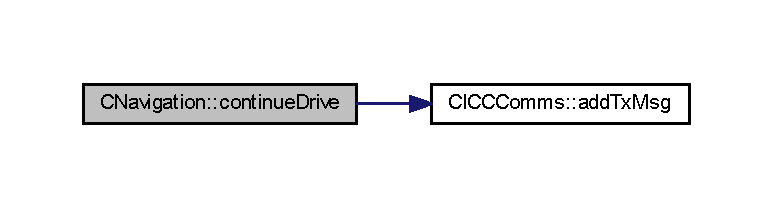
\includegraphics[width=350pt]{class_c_navigation_ab3d29f3ab4a8a922f5af439f6d78aded_cgraph}
\end{center}
\end{figure}
\mbox{\Hypertarget{class_c_navigation_a42982842952ac5340b54f43a661673f4}\label{class_c_navigation_a42982842952ac5340b54f43a661673f4}} 
\index{C\+Navigation@{C\+Navigation}!get\+Current\+State@{get\+Current\+State}}
\index{get\+Current\+State@{get\+Current\+State}!C\+Navigation@{C\+Navigation}}
\subsubsection{\texorpdfstring{get\+Current\+State()}{getCurrentState()}}
{\footnotesize\ttfamily \mbox{\hyperlink{class_c_navigation_add9fc966c7604990edf5c2a2e0eba32c}{C\+Navigation\+::\+N\+A\+V\+\_\+\+S\+T\+A\+TE}} C\+Navigation\+::get\+Current\+State (\begin{DoxyParamCaption}\item[{void}]{ }\end{DoxyParamCaption})\hspace{0.3cm}{\ttfamily [virtual]}}



Function to get current state. 

\begin{DoxyReturn}{Returns}
Returns current state as \mbox{\hyperlink{class_c_navigation_add9fc966c7604990edf5c2a2e0eba32c}{C\+Navigation\+::\+N\+A\+V\+\_\+\+S\+T\+A\+TE}} 
\end{DoxyReturn}


Definition at line 444 of file App\+\_\+\+Navigation.\+cpp.

\mbox{\Hypertarget{class_c_navigation_afef253f37646558a755d956ecf2fc6e9}\label{class_c_navigation_afef253f37646558a755d956ecf2fc6e9}} 
\index{C\+Navigation@{C\+Navigation}!get\+Next\+State@{get\+Next\+State}}
\index{get\+Next\+State@{get\+Next\+State}!C\+Navigation@{C\+Navigation}}
\subsubsection{\texorpdfstring{get\+Next\+State()}{getNextState()}}
{\footnotesize\ttfamily \mbox{\hyperlink{class_c_navigation_add9fc966c7604990edf5c2a2e0eba32c}{C\+Navigation\+::\+N\+A\+V\+\_\+\+S\+T\+A\+TE}} C\+Navigation\+::get\+Next\+State (\begin{DoxyParamCaption}\item[{void}]{ }\end{DoxyParamCaption})\hspace{0.3cm}{\ttfamily [virtual]}}



Function to get next state. 

\begin{DoxyReturn}{Returns}
Returns next state as \mbox{\hyperlink{class_c_navigation_add9fc966c7604990edf5c2a2e0eba32c}{C\+Navigation\+::\+N\+A\+V\+\_\+\+S\+T\+A\+TE}} 
\end{DoxyReturn}


Definition at line 453 of file App\+\_\+\+Navigation.\+cpp.

Here is the caller graph for this function\+:
\nopagebreak
\begin{figure}[H]
\begin{center}
\leavevmode
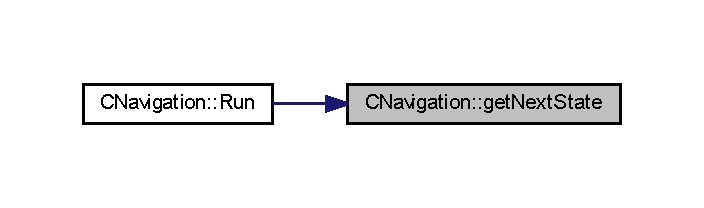
\includegraphics[width=338pt]{class_c_navigation_afef253f37646558a755d956ecf2fc6e9_icgraph}
\end{center}
\end{figure}
\mbox{\Hypertarget{class_c_navigation_a86a0756663ccf76e9c474764b8f7a04f}\label{class_c_navigation_a86a0756663ccf76e9c474764b8f7a04f}} 
\index{C\+Navigation@{C\+Navigation}!Init@{Init}}
\index{Init@{Init}!C\+Navigation@{C\+Navigation}}
\subsubsection{\texorpdfstring{Init()}{Init()}}
{\footnotesize\ttfamily void C\+Navigation\+::\+Init (\begin{DoxyParamCaption}\item[{void}]{ }\end{DoxyParamCaption})\hspace{0.3cm}{\ttfamily [virtual]}}



Initialization function of \mbox{\hyperlink{class_c_navigation}{C\+Navigation}}. 



Implements \mbox{\hyperlink{class_i_task___i_f_a28f608bdb9b19658403f7b9b7421968d}{I\+Task\+\_\+\+IF}}.



Definition at line 31 of file App\+\_\+\+Navigation.\+cpp.

\mbox{\Hypertarget{class_c_navigation_aa984fc062deefed13a85d866d997de73}\label{class_c_navigation_aa984fc062deefed13a85d866d997de73}} 
\index{C\+Navigation@{C\+Navigation}!is\+Corner\+Mode@{is\+Corner\+Mode}}
\index{is\+Corner\+Mode@{is\+Corner\+Mode}!C\+Navigation@{C\+Navigation}}
\subsubsection{\texorpdfstring{is\+Corner\+Mode()}{isCornerMode()}}
{\footnotesize\ttfamily bool C\+Navigation\+::is\+Corner\+Mode (\begin{DoxyParamCaption}{ }\end{DoxyParamCaption})}



Function to return if corner\+Mode is active. 

\begin{DoxyReturn}{Returns}
Returns current state of corner mode (active = true) 
\end{DoxyReturn}


Definition at line 78 of file App\+\_\+\+Navigation.\+cpp.

Here is the caller graph for this function\+:
\nopagebreak
\begin{figure}[H]
\begin{center}
\leavevmode
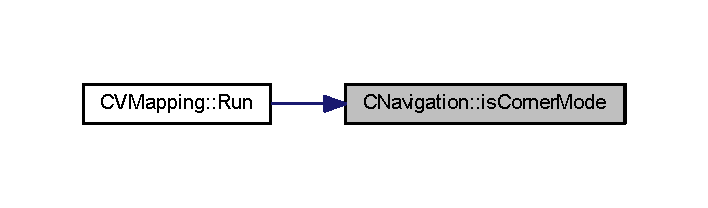
\includegraphics[width=340pt]{class_c_navigation_aa984fc062deefed13a85d866d997de73_icgraph}
\end{center}
\end{figure}
\mbox{\Hypertarget{class_c_navigation_a27649dc6324360829d42aea67e88e3ee}\label{class_c_navigation_a27649dc6324360829d42aea67e88e3ee}} 
\index{C\+Navigation@{C\+Navigation}!pause\+Drive@{pause\+Drive}}
\index{pause\+Drive@{pause\+Drive}!C\+Navigation@{C\+Navigation}}
\subsubsection{\texorpdfstring{pause\+Drive()}{pauseDrive()}}
{\footnotesize\ttfamily void C\+Navigation\+::pause\+Drive (\begin{DoxyParamCaption}\item[{void}]{ }\end{DoxyParamCaption})\hspace{0.3cm}{\ttfamily [virtual]}}



Pause drive due to obstacle detection. 



Definition at line 429 of file App\+\_\+\+Navigation.\+cpp.

Here is the call graph for this function\+:
\nopagebreak
\begin{figure}[H]
\begin{center}
\leavevmode
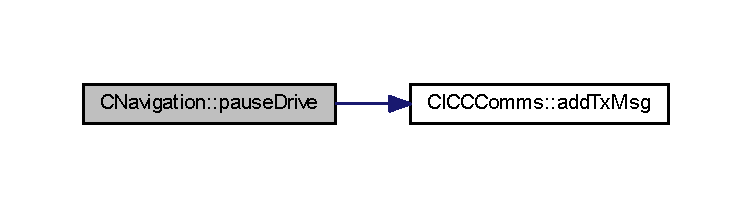
\includegraphics[width=350pt]{class_c_navigation_a27649dc6324360829d42aea67e88e3ee_cgraph}
\end{center}
\end{figure}
Here is the caller graph for this function\+:
\nopagebreak
\begin{figure}[H]
\begin{center}
\leavevmode
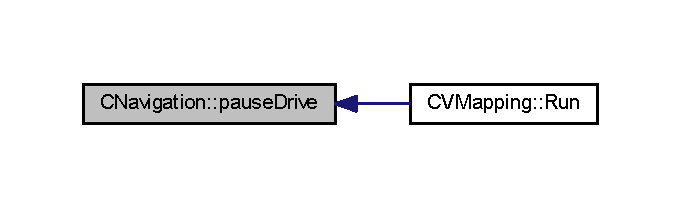
\includegraphics[width=327pt]{class_c_navigation_a27649dc6324360829d42aea67e88e3ee_icgraph}
\end{center}
\end{figure}
\mbox{\Hypertarget{class_c_navigation_ac491c77788ba2e953a704b6ad622a665}\label{class_c_navigation_ac491c77788ba2e953a704b6ad622a665}} 
\index{C\+Navigation@{C\+Navigation}!print\+Changed\+Debug\+Info@{print\+Changed\+Debug\+Info}}
\index{print\+Changed\+Debug\+Info@{print\+Changed\+Debug\+Info}!C\+Navigation@{C\+Navigation}}
\subsubsection{\texorpdfstring{print\+Changed\+Debug\+Info()}{printChangedDebugInfo()}}
{\footnotesize\ttfamily void C\+Navigation\+::print\+Changed\+Debug\+Info (\begin{DoxyParamCaption}\item[{void}]{ }\end{DoxyParamCaption})\hspace{0.3cm}{\ttfamily [virtual]}}



Debug function to print current status of state flow if changed. 



Definition at line 199 of file App\+\_\+\+Navigation.\+cpp.

Here is the call graph for this function\+:
\nopagebreak
\begin{figure}[H]
\begin{center}
\leavevmode
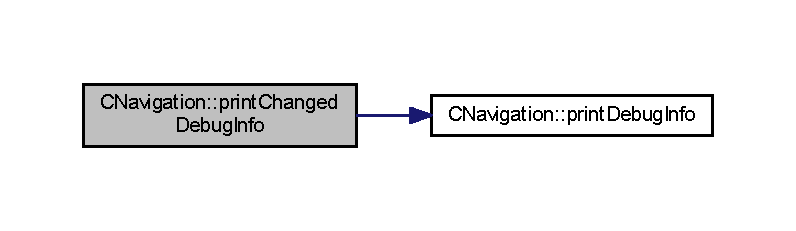
\includegraphics[width=350pt]{class_c_navigation_ac491c77788ba2e953a704b6ad622a665_cgraph}
\end{center}
\end{figure}
Here is the caller graph for this function\+:
\nopagebreak
\begin{figure}[H]
\begin{center}
\leavevmode
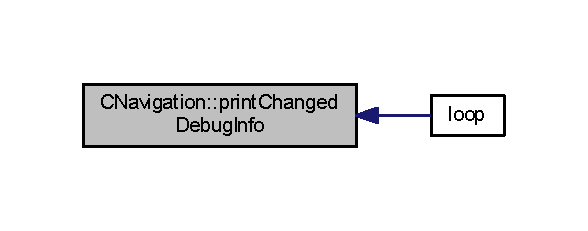
\includegraphics[width=282pt]{class_c_navigation_ac491c77788ba2e953a704b6ad622a665_icgraph}
\end{center}
\end{figure}
\mbox{\Hypertarget{class_c_navigation_a84e320cd8975593ab6f966e8794b2886}\label{class_c_navigation_a84e320cd8975593ab6f966e8794b2886}} 
\index{C\+Navigation@{C\+Navigation}!print\+Debug\+Info@{print\+Debug\+Info}}
\index{print\+Debug\+Info@{print\+Debug\+Info}!C\+Navigation@{C\+Navigation}}
\subsubsection{\texorpdfstring{print\+Debug\+Info()}{printDebugInfo()}}
{\footnotesize\ttfamily void C\+Navigation\+::print\+Debug\+Info (\begin{DoxyParamCaption}\item[{void}]{ }\end{DoxyParamCaption})\hspace{0.3cm}{\ttfamily [virtual]}}



Debug function to print current status of state flow. 



Definition at line 226 of file App\+\_\+\+Navigation.\+cpp.

Here is the caller graph for this function\+:
\nopagebreak
\begin{figure}[H]
\begin{center}
\leavevmode
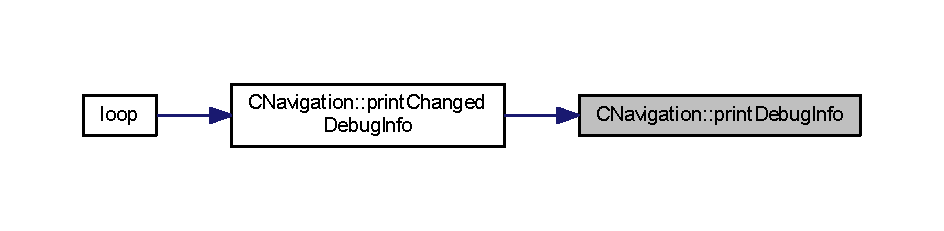
\includegraphics[width=350pt]{class_c_navigation_a84e320cd8975593ab6f966e8794b2886_icgraph}
\end{center}
\end{figure}
\mbox{\Hypertarget{class_c_navigation_a86acb1521aab400e542465c8eabed671}\label{class_c_navigation_a86acb1521aab400e542465c8eabed671}} 
\index{C\+Navigation@{C\+Navigation}!Run@{Run}}
\index{Run@{Run}!C\+Navigation@{C\+Navigation}}
\subsubsection{\texorpdfstring{Run()}{Run()}}
{\footnotesize\ttfamily void C\+Navigation\+::\+Run (\begin{DoxyParamCaption}\item[{void}]{ }\end{DoxyParamCaption})\hspace{0.3cm}{\ttfamily [virtual]}}



Run function of \mbox{\hyperlink{class_c_navigation}{C\+Navigation}} which is periodically called by \mbox{\hyperlink{class_c_task_ctrl}{C\+Task\+Ctrl}}. 

Reads data from I\+CC, gets data from P\+LS and calculates navigation. 

Implements \mbox{\hyperlink{class_i_task___i_f_ab73cc5879a61d00fc59b72cce32cc6f7}{I\+Task\+\_\+\+IF}}.



Definition at line 40 of file App\+\_\+\+Navigation.\+cpp.

Here is the call graph for this function\+:
\nopagebreak
\begin{figure}[H]
\begin{center}
\leavevmode
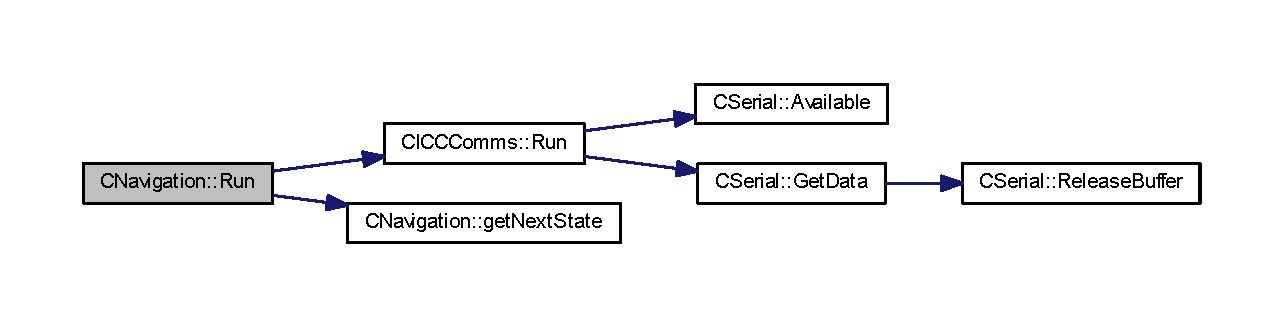
\includegraphics[width=350pt]{class_c_navigation_a86acb1521aab400e542465c8eabed671_cgraph}
\end{center}
\end{figure}
\mbox{\Hypertarget{class_c_navigation_a53f0409677e36f62ef232f7e15b32948}\label{class_c_navigation_a53f0409677e36f62ef232f7e15b32948}} 
\index{C\+Navigation@{C\+Navigation}!set\+P\+L\+Sdata@{set\+P\+L\+Sdata}}
\index{set\+P\+L\+Sdata@{set\+P\+L\+Sdata}!C\+Navigation@{C\+Navigation}}
\subsubsection{\texorpdfstring{set\+P\+L\+Sdata()}{setPLSdata()}}
{\footnotesize\ttfamily void C\+Navigation\+::set\+P\+L\+Sdata (\begin{DoxyParamCaption}\item[{\mbox{\hyperlink{_a_d_a_s___types_8h_a1f1825b69244eb3ad2c7165ddc99c956}{uint16\+\_\+t}}}]{offset,  }\item[{int8\+\_\+t}]{angle,  }\item[{\mbox{\hyperlink{_a_d_a_s___types_8h_a1f1825b69244eb3ad2c7165ddc99c956}{uint16\+\_\+t}}}]{nxt\+\_\+wall }\end{DoxyParamCaption})\hspace{0.3cm}{\ttfamily [virtual]}}



Function to set the current value of offset position to wall, current angle of the wall and current distance to wall in front to the input buffer. 


\begin{DoxyParams}{Parameters}
{\em offset} & Offset to right wall in cm \\
\hline
{\em angle} & Angle of right wall in degrees \\
\hline
{\em nxt\+\_\+wall} & Distance to wall in front in cm \\
\hline
\end{DoxyParams}


Definition at line 89 of file App\+\_\+\+Navigation.\+cpp.

Here is the caller graph for this function\+:
\nopagebreak
\begin{figure}[H]
\begin{center}
\leavevmode
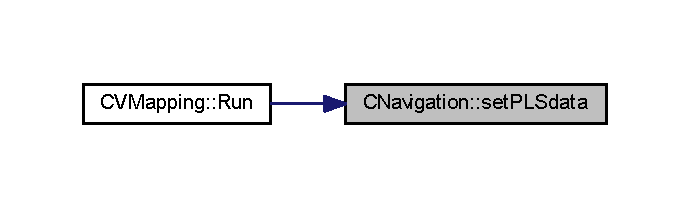
\includegraphics[width=331pt]{class_c_navigation_a53f0409677e36f62ef232f7e15b32948_icgraph}
\end{center}
\end{figure}
\mbox{\Hypertarget{class_c_navigation_a3cc8f7fdd003d6b2c5056b87ff93edd9}\label{class_c_navigation_a3cc8f7fdd003d6b2c5056b87ff93edd9}} 
\index{C\+Navigation@{C\+Navigation}!Stop@{Stop}}
\index{Stop@{Stop}!C\+Navigation@{C\+Navigation}}
\subsubsection{\texorpdfstring{Stop()}{Stop()}}
{\footnotesize\ttfamily void C\+Navigation\+::\+Stop (\begin{DoxyParamCaption}\item[{void}]{ }\end{DoxyParamCaption})\hspace{0.3cm}{\ttfamily [virtual]}}



Stop function of \mbox{\hyperlink{class_c_navigation}{C\+Navigation}}. 



Implements \mbox{\hyperlink{class_i_task___i_f_af5f8fba86704c7e36d0e4681d58300c6}{I\+Task\+\_\+\+IF}}.



Definition at line 64 of file App\+\_\+\+Navigation.\+cpp.

Here is the call graph for this function\+:
\nopagebreak
\begin{figure}[H]
\begin{center}
\leavevmode
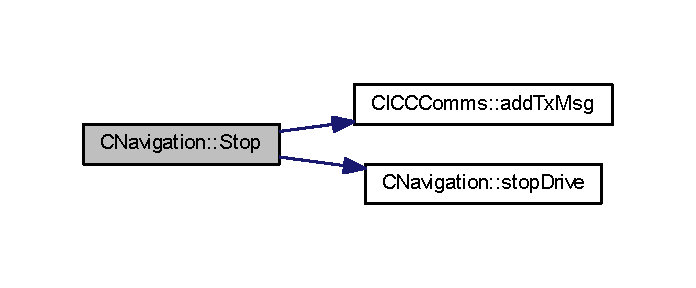
\includegraphics[width=334pt]{class_c_navigation_a3cc8f7fdd003d6b2c5056b87ff93edd9_cgraph}
\end{center}
\end{figure}
\mbox{\Hypertarget{class_c_navigation_a06ce71124d487f1f9febf36a0e4b2a5d}\label{class_c_navigation_a06ce71124d487f1f9febf36a0e4b2a5d}} 
\index{C\+Navigation@{C\+Navigation}!stop\+Drive@{stop\+Drive}}
\index{stop\+Drive@{stop\+Drive}!C\+Navigation@{C\+Navigation}}
\subsubsection{\texorpdfstring{stop\+Drive()}{stopDrive()}}
{\footnotesize\ttfamily void C\+Navigation\+::stop\+Drive (\begin{DoxyParamCaption}\item[{void}]{ }\end{DoxyParamCaption})\hspace{0.3cm}{\ttfamily [virtual]}}



Function to stop if obstacle is detected. 



Definition at line 328 of file App\+\_\+\+Navigation.\+cpp.

Here is the caller graph for this function\+:
\nopagebreak
\begin{figure}[H]
\begin{center}
\leavevmode
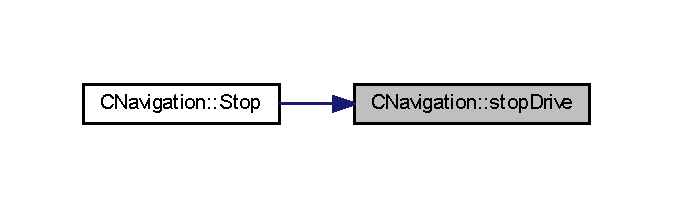
\includegraphics[width=323pt]{class_c_navigation_a06ce71124d487f1f9febf36a0e4b2a5d_icgraph}
\end{center}
\end{figure}


\subsection{Member Data Documentation}
\mbox{\Hypertarget{class_c_navigation_af3f718b7aa00a149c31c5682113da75e}\label{class_c_navigation_af3f718b7aa00a149c31c5682113da75e}} 
\index{C\+Navigation@{C\+Navigation}!distance\+Done@{distance\+Done}}
\index{distance\+Done@{distance\+Done}!C\+Navigation@{C\+Navigation}}
\subsubsection{\texorpdfstring{distance\+Done}{distanceDone}}
{\footnotesize\ttfamily volatile bool C\+Navigation\+::distance\+Done}

Parameter to show that distance is reached 

Definition at line 94 of file App\+\_\+\+Navigation.\+h.

\mbox{\Hypertarget{class_c_navigation_a069e02947303fed95655cd4ad88a96b7}\label{class_c_navigation_a069e02947303fed95655cd4ad88a96b7}} 
\index{C\+Navigation@{C\+Navigation}!rotation\+Done@{rotation\+Done}}
\index{rotation\+Done@{rotation\+Done}!C\+Navigation@{C\+Navigation}}
\subsubsection{\texorpdfstring{rotation\+Done}{rotationDone}}
{\footnotesize\ttfamily volatile bool C\+Navigation\+::rotation\+Done}

Parameter to show that rotation is finished 

Definition at line 89 of file App\+\_\+\+Navigation.\+h.



The documentation for this class was generated from the following files\+:\begin{DoxyCompactItemize}
\item 
\mbox{\hyperlink{_app___navigation_8h}{App\+\_\+\+Navigation.\+h}}\item 
\mbox{\hyperlink{_app___navigation_8cpp}{App\+\_\+\+Navigation.\+cpp}}\end{DoxyCompactItemize}

\hypertarget{class_c_p_l_s_comms}{}\section{C\+P\+L\+S\+Comms Class Reference}
\label{class_c_p_l_s_comms}\index{CPLSComms@{CPLSComms}}
\subsection*{Classes}
\begin{DoxyCompactItemize}
\item 
struct \mbox{\hyperlink{struct_c_p_l_s_comms_1_1_message__t}{Message\+\_\+t}}
\end{DoxyCompactItemize}
\subsection*{Public Types}
\begin{DoxyCompactItemize}
\item 
\mbox{\Hypertarget{class_c_p_l_s_comms_a765bc36363f75f4faf4fd2b41d440159}\label{class_c_p_l_s_comms_a765bc36363f75f4faf4fd2b41d440159}} 
enum {\bfseries Status\+\_\+e} \{ \newline
{\bfseries Msg\+Success} =0, 
{\bfseries C\+R\+C\+Check\+Fail} = 1, 
{\bfseries Comms\+Error} = 2, 
{\bfseries Partial\+Msg} = 3, 
\newline
{\bfseries Msg\+\_\+\+N\+CK} =4, 
{\bfseries Invalid\+Req} =5
 \}
\end{DoxyCompactItemize}
\subsection*{Public Member Functions}
\begin{DoxyCompactItemize}
\item 
\mbox{\Hypertarget{class_c_p_l_s_comms_ae1ec975e5e402b405389d47b8acd0a63}\label{class_c_p_l_s_comms_ae1ec975e5e402b405389d47b8acd0a63}} 
{\bfseries C\+P\+L\+S\+Comms} (\mbox{\hyperlink{class_c_serial}{C\+Serial}} \&ser\+Port)
\item 
\mbox{\Hypertarget{class_c_p_l_s_comms_ae7f8d87ea15de35a120d65a7a8bbbb76}\label{class_c_p_l_s_comms_ae7f8d87ea15de35a120d65a7a8bbbb76}} 
Status\+\_\+e {\bfseries Init} (void)
\item 
\mbox{\Hypertarget{class_c_p_l_s_comms_ae8f7e9acdf4243b76f3c7f61cf766cfc}\label{class_c_p_l_s_comms_ae8f7e9acdf4243b76f3c7f61cf766cfc}} 
void {\bfseries Request\+Measurements} (bool only\+Vert)
\item 
\mbox{\Hypertarget{class_c_p_l_s_comms_a3124eaa4549706962c7024c7c97e82b0}\label{class_c_p_l_s_comms_a3124eaa4549706962c7024c7c97e82b0}} 
bool {\bfseries Get\+Async\+Data} (\mbox{\hyperlink{struct_c_p_l_s_comms_1_1_message__t}{Message\+\_\+t}} \&msg, uint16\+\_\+t \&len)
\item 
\mbox{\Hypertarget{class_c_p_l_s_comms_ae9d000eff184034954829d76162654a5}\label{class_c_p_l_s_comms_ae9d000eff184034954829d76162654a5}} 
bool {\bfseries Data\+Available} ()
\item 
\mbox{\Hypertarget{class_c_p_l_s_comms_a05149da99ab80b804699763111315f33}\label{class_c_p_l_s_comms_a05149da99ab80b804699763111315f33}} 
Status\+\_\+e {\bfseries Get\+Status} (void)
\item 
\mbox{\Hypertarget{class_c_p_l_s_comms_ae0cd51de8a24b261389b6f89b4b80e51}\label{class_c_p_l_s_comms_ae0cd51de8a24b261389b6f89b4b80e51}} 
bool {\bfseries Search\+Msg} (\mbox{\hyperlink{struct_c_p_l_s_comms_1_1_message__t}{Message\+\_\+t}} \&msg, uint8\+\_\+t ID, uint16\+\_\+t len)
\end{DoxyCompactItemize}


\subsection{Detailed Description}


Definition at line 16 of file Comm\+\_\+\+P\+L\+S.\+h.



The documentation for this class was generated from the following files\+:\begin{DoxyCompactItemize}
\item 
/\+Volumes/\+Macintosh S\+D/\+Github/\+A\+D\+A\+S/06\+\_\+source/\+A\+D\+A\+S/\+A\+D\+A\+S\+\_\+\+Nav\+U/Comm\+\_\+\+P\+L\+S.\+h\item 
/\+Volumes/\+Macintosh S\+D/\+Github/\+A\+D\+A\+S/06\+\_\+source/\+A\+D\+A\+S/\+A\+D\+A\+S\+\_\+\+Nav\+U/Comm\+\_\+\+P\+L\+S.\+cpp\end{DoxyCompactItemize}

\hypertarget{class_c_positioning}{}\section{C\+Positioning Class Reference}
\label{class_c_positioning}\index{C\+Positioning@{C\+Positioning}}


{\ttfamily \#include $<$App\+\_\+\+Positioning.\+h$>$}



Inheritance diagram for C\+Positioning\+:
\nopagebreak
\begin{figure}[H]
\begin{center}
\leavevmode
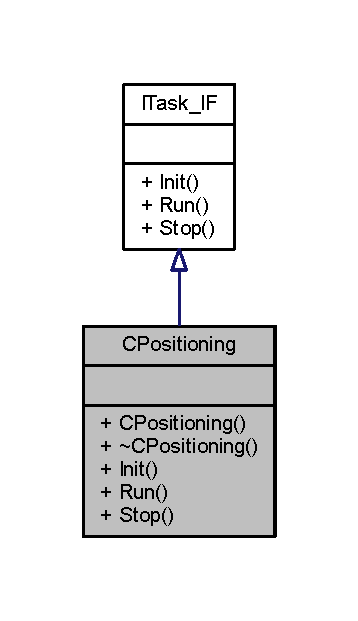
\includegraphics[width=172pt]{class_c_positioning__inherit__graph}
\end{center}
\end{figure}


Collaboration diagram for C\+Positioning\+:
\nopagebreak
\begin{figure}[H]
\begin{center}
\leavevmode
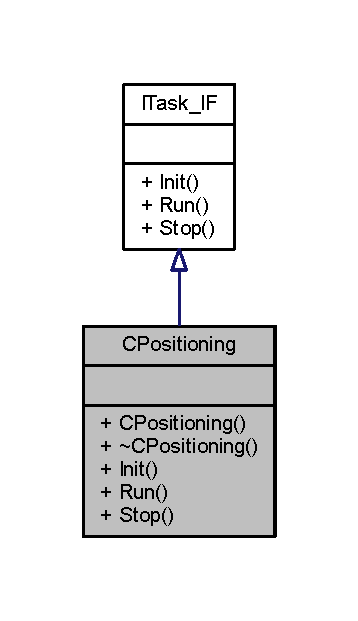
\includegraphics[width=172pt]{class_c_positioning__coll__graph}
\end{center}
\end{figure}
\subsection*{Public Member Functions}
\begin{DoxyCompactItemize}
\item 
\mbox{\hyperlink{class_c_positioning_a2ef1dd3d4755b30ac7b800876de70869}{C\+Positioning}} ()
\begin{DoxyCompactList}\small\item\em position app class constructor. \end{DoxyCompactList}\item 
\mbox{\hyperlink{class_c_positioning_a2d1846176104d85f119010a471f6483d}{$\sim$\+C\+Positioning}} ()
\begin{DoxyCompactList}\small\item\em position app class destructor. \end{DoxyCompactList}\item 
virtual void \mbox{\hyperlink{class_c_positioning_abdceba66e701554a178acf61c61b0df6}{Init}} (void)
\begin{DoxyCompactList}\small\item\em Initialization function of Positioning Application. \end{DoxyCompactList}\item 
virtual void \mbox{\hyperlink{class_c_positioning_ad0e439dcc95c450548c2806077aeff57}{Run}} (void)
\begin{DoxyCompactList}\small\item\em Run function of Positioning Application. \end{DoxyCompactList}\item 
virtual void \mbox{\hyperlink{class_c_positioning_a2706c9bb6bb52201c279386fd2c9dd89}{Stop}} (void)
\begin{DoxyCompactList}\small\item\em Stop/shutdown function of Positioning Application. \end{DoxyCompactList}\end{DoxyCompactItemize}


\subsection{Detailed Description}
Template class positioning contains only basic functionality required by task controller 

Definition at line 19 of file App\+\_\+\+Positioning.\+h.



\subsection{Constructor \& Destructor Documentation}
\mbox{\Hypertarget{class_c_positioning_a2ef1dd3d4755b30ac7b800876de70869}\label{class_c_positioning_a2ef1dd3d4755b30ac7b800876de70869}} 
\index{C\+Positioning@{C\+Positioning}!C\+Positioning@{C\+Positioning}}
\index{C\+Positioning@{C\+Positioning}!C\+Positioning@{C\+Positioning}}
\subsubsection{\texorpdfstring{C\+Positioning()}{CPositioning()}}
{\footnotesize\ttfamily C\+Positioning\+::\+C\+Positioning (\begin{DoxyParamCaption}{ }\end{DoxyParamCaption})}



position app class constructor. 



Definition at line 14 of file App\+\_\+\+Positioning.\+cpp.

\mbox{\Hypertarget{class_c_positioning_a2d1846176104d85f119010a471f6483d}\label{class_c_positioning_a2d1846176104d85f119010a471f6483d}} 
\index{C\+Positioning@{C\+Positioning}!````~C\+Positioning@{$\sim$\+C\+Positioning}}
\index{````~C\+Positioning@{$\sim$\+C\+Positioning}!C\+Positioning@{C\+Positioning}}
\subsubsection{\texorpdfstring{$\sim$\+C\+Positioning()}{~CPositioning()}}
{\footnotesize\ttfamily C\+Positioning\+::$\sim$\+C\+Positioning (\begin{DoxyParamCaption}{ }\end{DoxyParamCaption})}



position app class destructor. 



Definition at line 20 of file App\+\_\+\+Positioning.\+cpp.



\subsection{Member Function Documentation}
\mbox{\Hypertarget{class_c_positioning_abdceba66e701554a178acf61c61b0df6}\label{class_c_positioning_abdceba66e701554a178acf61c61b0df6}} 
\index{C\+Positioning@{C\+Positioning}!Init@{Init}}
\index{Init@{Init}!C\+Positioning@{C\+Positioning}}
\subsubsection{\texorpdfstring{Init()}{Init()}}
{\footnotesize\ttfamily void C\+Positioning\+::\+Init (\begin{DoxyParamCaption}\item[{void}]{ }\end{DoxyParamCaption})\hspace{0.3cm}{\ttfamily [virtual]}}



Initialization function of Positioning Application. 

Realization of pure virtual function task\+\_\+\+IF Called by task controller for initializing applications 

Implements \mbox{\hyperlink{class_i_task___i_f_a28f608bdb9b19658403f7b9b7421968d}{I\+Task\+\_\+\+IF}}.



Definition at line 25 of file App\+\_\+\+Positioning.\+cpp.

\mbox{\Hypertarget{class_c_positioning_ad0e439dcc95c450548c2806077aeff57}\label{class_c_positioning_ad0e439dcc95c450548c2806077aeff57}} 
\index{C\+Positioning@{C\+Positioning}!Run@{Run}}
\index{Run@{Run}!C\+Positioning@{C\+Positioning}}
\subsubsection{\texorpdfstring{Run()}{Run()}}
{\footnotesize\ttfamily void C\+Positioning\+::\+Run (\begin{DoxyParamCaption}\item[{void}]{ }\end{DoxyParamCaption})\hspace{0.3cm}{\ttfamily [virtual]}}



Run function of Positioning Application. 

Realization of pure virtual function task\+\_\+\+IF Called by task controller for running functionality 

Implements \mbox{\hyperlink{class_i_task___i_f_ab73cc5879a61d00fc59b72cce32cc6f7}{I\+Task\+\_\+\+IF}}.



Definition at line 31 of file App\+\_\+\+Positioning.\+cpp.

\mbox{\Hypertarget{class_c_positioning_a2706c9bb6bb52201c279386fd2c9dd89}\label{class_c_positioning_a2706c9bb6bb52201c279386fd2c9dd89}} 
\index{C\+Positioning@{C\+Positioning}!Stop@{Stop}}
\index{Stop@{Stop}!C\+Positioning@{C\+Positioning}}
\subsubsection{\texorpdfstring{Stop()}{Stop()}}
{\footnotesize\ttfamily void C\+Positioning\+::\+Stop (\begin{DoxyParamCaption}\item[{void}]{ }\end{DoxyParamCaption})\hspace{0.3cm}{\ttfamily [virtual]}}



Stop/shutdown function of Positioning Application. 

Realization of pure virtual function task\+\_\+\+IF Called by task controller for shutdown 

Implements \mbox{\hyperlink{class_i_task___i_f_af5f8fba86704c7e36d0e4681d58300c6}{I\+Task\+\_\+\+IF}}.



Definition at line 37 of file App\+\_\+\+Positioning.\+cpp.



The documentation for this class was generated from the following files\+:\begin{DoxyCompactItemize}
\item 
\mbox{\hyperlink{_app___positioning_8h}{App\+\_\+\+Positioning.\+h}}\item 
\mbox{\hyperlink{_app___positioning_8cpp}{App\+\_\+\+Positioning.\+cpp}}\end{DoxyCompactItemize}

\hypertarget{class_c_serial}{}\section{C\+Serial Class Reference}
\label{class_c_serial}\index{CSerial@{CSerial}}


Hardware Abstraction Layer (H\+AL) Serial class.  




{\ttfamily \#include $<$H\+A\+L\+\_\+\+Serial\+\_\+\+I\+F.\+h$>$}



Collaboration diagram for C\+Serial\+:\nopagebreak
\begin{figure}[H]
\begin{center}
\leavevmode
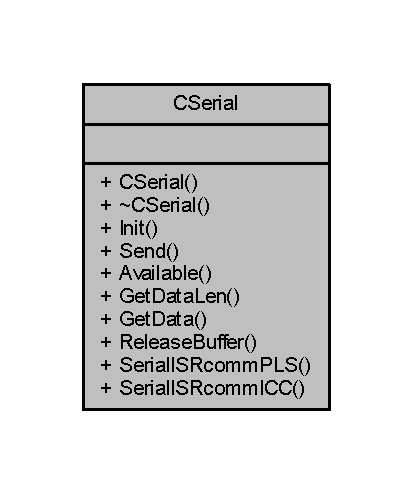
\includegraphics[width=198pt]{class_c_serial__coll__graph}
\end{center}
\end{figure}
\subsection*{Public Types}
\begin{DoxyCompactItemize}
\item 
enum \mbox{\hyperlink{class_c_serial_a000039540cc90b18bafacf5744e7eda2}{Port\+I\+D\+\_\+e}} \{ \mbox{\hyperlink{class_c_serial_a000039540cc90b18bafacf5744e7eda2a2a245d3c55e5b6e7052daf261924ce08}{S1}}, 
\mbox{\hyperlink{class_c_serial_a000039540cc90b18bafacf5744e7eda2a8cc95f4591147b0df028e003f82220a1}{S2}}
 \}
\begin{DoxyCompactList}\small\item\em Serial interface definition. \end{DoxyCompactList}\end{DoxyCompactItemize}
\subsection*{Public Member Functions}
\begin{DoxyCompactItemize}
\item 
\mbox{\hyperlink{class_c_serial_a3b2b31de1529b884b8d5e354586ee981}{C\+Serial}} (\mbox{\hyperlink{class_c_serial_a000039540cc90b18bafacf5744e7eda2}{Port\+I\+D\+\_\+e}} i\+\_\+\+ID, \mbox{\hyperlink{_a_d_a_s___types_8h_a1f1825b69244eb3ad2c7165ddc99c956}{uint16\+\_\+t}} i\+\_\+buf\+Len)
\begin{DoxyCompactList}\small\item\em Constructor of \mbox{\hyperlink{class_c_serial}{C\+Serial}}. \end{DoxyCompactList}\item 
\mbox{\hyperlink{class_c_serial_aff5444dd7e6a9ddc43cbce0e959edf7a}{$\sim$\+C\+Serial}} ()
\begin{DoxyCompactList}\small\item\em Destructor of \mbox{\hyperlink{class_c_serial}{C\+Serial}}. \end{DoxyCompactList}\item 
void \mbox{\hyperlink{class_c_serial_aed500bd204c4b37665d6d228333edafb}{Init}} (void)
\begin{DoxyCompactList}\small\item\em Initialization function of \mbox{\hyperlink{class_c_serial}{C\+Serial}}. \end{DoxyCompactList}\item 
bool \mbox{\hyperlink{class_c_serial_ae5bec6d6a1c75839ae02cf0069d1f08e}{Send}} (char Buff\mbox{[}$\,$\mbox{]}, \mbox{\hyperlink{_a_d_a_s___types_8h_aba7bc1797add20fe3efdf37ced1182c5}{uint8\+\_\+t}} len)
\begin{DoxyCompactList}\small\item\em Function to send data in transmit buffer. \end{DoxyCompactList}\item 
bool \mbox{\hyperlink{class_c_serial_abb43734223d937a86e7616636ea16024}{Available}} (void)
\begin{DoxyCompactList}\small\item\em Function to check availability of received data. \end{DoxyCompactList}\item 
\mbox{\hyperlink{_a_d_a_s___types_8h_a1f1825b69244eb3ad2c7165ddc99c956}{uint16\+\_\+t}} \mbox{\hyperlink{class_c_serial_a4327d6041fe9a390612b214709027cbb}{Get\+Data\+Len}} (void)
\begin{DoxyCompactList}\small\item\em Function to get length of data. \end{DoxyCompactList}\item 
bool \mbox{\hyperlink{class_c_serial_abad86c07f530569b2ceeea75bda485ad}{Get\+Data}} (\mbox{\hyperlink{_a_d_a_s___types_8h_aba7bc1797add20fe3efdf37ced1182c5}{uint8\+\_\+t}} $\ast$data, \mbox{\hyperlink{_a_d_a_s___types_8h_a1f1825b69244eb3ad2c7165ddc99c956}{uint16\+\_\+t}} len)
\begin{DoxyCompactList}\small\item\em Function to read data from buffer. \end{DoxyCompactList}\item 
void \mbox{\hyperlink{class_c_serial_a941e5cae2ca04518925a3b32f51110a6}{Release\+Buffer}} (void)
\begin{DoxyCompactList}\small\item\em Function to release buffer. \end{DoxyCompactList}\item 
void \mbox{\hyperlink{class_c_serial_a707841754d94fc1ab6679f52bf413d85}{Serial\+I\+S\+Rcomm\+P\+LS}} (void)
\begin{DoxyCompactList}\small\item\em Function for I\+SR U\+S\+A\+R\+Tn\+\_\+\+R\+X\+\_\+vect for P\+LS communication. \end{DoxyCompactList}\item 
void \mbox{\hyperlink{class_c_serial_a974812db5ced18cb9a6a73dc9034e7c8}{Serial\+I\+S\+Rcomm\+I\+CC}} (void)
\begin{DoxyCompactList}\small\item\em Function for I\+SR U\+S\+A\+R\+Tn\+\_\+\+R\+X\+\_\+vect for inter-\/controller communication. \end{DoxyCompactList}\end{DoxyCompactItemize}


\subsection{Detailed Description}
Hardware Abstraction Layer (H\+AL) Serial class. 

Definition at line 15 of file H\+A\+L\+\_\+\+Serial\+\_\+\+I\+F.\+h.



\subsection{Member Enumeration Documentation}
\mbox{\Hypertarget{class_c_serial_a000039540cc90b18bafacf5744e7eda2}\label{class_c_serial_a000039540cc90b18bafacf5744e7eda2}} 
\index{CSerial@{CSerial}!PortID\_e@{PortID\_e}}
\index{PortID\_e@{PortID\_e}!CSerial@{CSerial}}
\subsubsection{\texorpdfstring{PortID\_e}{PortID\_e}}
{\footnotesize\ttfamily enum \mbox{\hyperlink{class_c_serial_a000039540cc90b18bafacf5744e7eda2}{C\+Serial\+::\+Port\+I\+D\+\_\+e}}}



Serial interface definition. 

\begin{DoxyEnumFields}{Enumerator}
\raisebox{\heightof{T}}[0pt][0pt]{\index{S1@{S1}!CSerial@{CSerial}}\index{CSerial@{CSerial}!S1@{S1}}}\mbox{\Hypertarget{class_c_serial_a000039540cc90b18bafacf5744e7eda2a2a245d3c55e5b6e7052daf261924ce08}\label{class_c_serial_a000039540cc90b18bafacf5744e7eda2a2a245d3c55e5b6e7052daf261924ce08}} 
S1&Serial interface 1 \\
\hline

\raisebox{\heightof{T}}[0pt][0pt]{\index{S2@{S2}!CSerial@{CSerial}}\index{CSerial@{CSerial}!S2@{S2}}}\mbox{\Hypertarget{class_c_serial_a000039540cc90b18bafacf5744e7eda2a8cc95f4591147b0df028e003f82220a1}\label{class_c_serial_a000039540cc90b18bafacf5744e7eda2a8cc95f4591147b0df028e003f82220a1}} 
S2&Serial interface 2 \\
\hline

\end{DoxyEnumFields}


Definition at line 22 of file H\+A\+L\+\_\+\+Serial\+\_\+\+I\+F.\+h.



\subsection{Constructor \& Destructor Documentation}
\mbox{\Hypertarget{class_c_serial_a3b2b31de1529b884b8d5e354586ee981}\label{class_c_serial_a3b2b31de1529b884b8d5e354586ee981}} 
\index{CSerial@{CSerial}!CSerial@{CSerial}}
\index{CSerial@{CSerial}!CSerial@{CSerial}}
\subsubsection{\texorpdfstring{CSerial()}{CSerial()}}
{\footnotesize\ttfamily C\+Serial\+::\+C\+Serial (\begin{DoxyParamCaption}\item[{\mbox{\hyperlink{class_c_serial_a000039540cc90b18bafacf5744e7eda2}{Port\+I\+D\+\_\+e}}}]{i\+\_\+\+ID,  }\item[{\mbox{\hyperlink{_a_d_a_s___types_8h_a1f1825b69244eb3ad2c7165ddc99c956}{uint16\+\_\+t}}}]{i\+\_\+buf\+Len }\end{DoxyParamCaption})}



Constructor of \mbox{\hyperlink{class_c_serial}{C\+Serial}}. 


\begin{DoxyParams}{Parameters}
{\em i\+\_\+\+ID} & Selection of serial interace e.\+g. S1 for Serial interface 1 \\
\hline
{\em i\+\_\+buf\+Len} & Length of receiving buffer \\
\hline
\end{DoxyParams}


Definition at line 19 of file H\+A\+L\+\_\+\+Serial\+\_\+\+I\+F.\+cpp.

\mbox{\Hypertarget{class_c_serial_aff5444dd7e6a9ddc43cbce0e959edf7a}\label{class_c_serial_aff5444dd7e6a9ddc43cbce0e959edf7a}} 
\index{CSerial@{CSerial}!````~CSerial@{$\sim$CSerial}}
\index{````~CSerial@{$\sim$CSerial}!CSerial@{CSerial}}
\subsubsection{\texorpdfstring{$\sim$CSerial()}{~CSerial()}}
{\footnotesize\ttfamily C\+Serial\+::$\sim$\+C\+Serial (\begin{DoxyParamCaption}{ }\end{DoxyParamCaption})}



Destructor of \mbox{\hyperlink{class_c_serial}{C\+Serial}}. 



Definition at line 30 of file H\+A\+L\+\_\+\+Serial\+\_\+\+I\+F.\+cpp.



\subsection{Member Function Documentation}
\mbox{\Hypertarget{class_c_serial_abb43734223d937a86e7616636ea16024}\label{class_c_serial_abb43734223d937a86e7616636ea16024}} 
\index{CSerial@{CSerial}!Available@{Available}}
\index{Available@{Available}!CSerial@{CSerial}}
\subsubsection{\texorpdfstring{Available()}{Available()}}
{\footnotesize\ttfamily bool C\+Serial\+::\+Available (\begin{DoxyParamCaption}\item[{void}]{ }\end{DoxyParamCaption})}



Function to check availability of received data. 

\begin{DoxyReturn}{Returns}
Returns a true if data in buffer is available 
\end{DoxyReturn}


Definition at line 128 of file H\+A\+L\+\_\+\+Serial\+\_\+\+I\+F.\+cpp.

Here is the caller graph for this function\+:\nopagebreak
\begin{figure}[H]
\begin{center}
\leavevmode
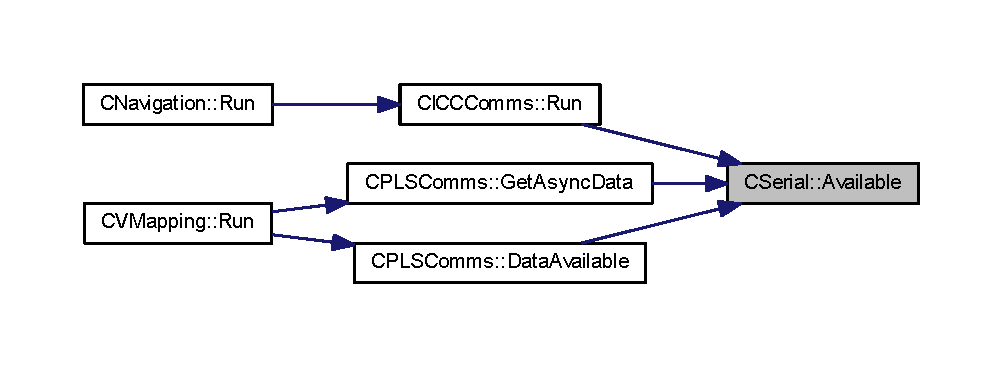
\includegraphics[width=350pt]{class_c_serial_abb43734223d937a86e7616636ea16024_icgraph}
\end{center}
\end{figure}
\mbox{\Hypertarget{class_c_serial_abad86c07f530569b2ceeea75bda485ad}\label{class_c_serial_abad86c07f530569b2ceeea75bda485ad}} 
\index{CSerial@{CSerial}!GetData@{GetData}}
\index{GetData@{GetData}!CSerial@{CSerial}}
\subsubsection{\texorpdfstring{GetData()}{GetData()}}
{\footnotesize\ttfamily bool C\+Serial\+::\+Get\+Data (\begin{DoxyParamCaption}\item[{\mbox{\hyperlink{_a_d_a_s___types_8h_aba7bc1797add20fe3efdf37ced1182c5}{uint8\+\_\+t}} $\ast$}]{data,  }\item[{\mbox{\hyperlink{_a_d_a_s___types_8h_a1f1825b69244eb3ad2c7165ddc99c956}{uint16\+\_\+t}}}]{len }\end{DoxyParamCaption})}



Function to read data from buffer. 


\begin{DoxyParams}{Parameters}
{\em data} & Pointer to destination where data shall be saved \\
\hline
{\em len} & Length of received data \\
\hline
\end{DoxyParams}
\begin{DoxyReturn}{Returns}
Returns a true of data is read 
\end{DoxyReturn}


Definition at line 148 of file H\+A\+L\+\_\+\+Serial\+\_\+\+I\+F.\+cpp.

Here is the call graph for this function\+:\nopagebreak
\begin{figure}[H]
\begin{center}
\leavevmode
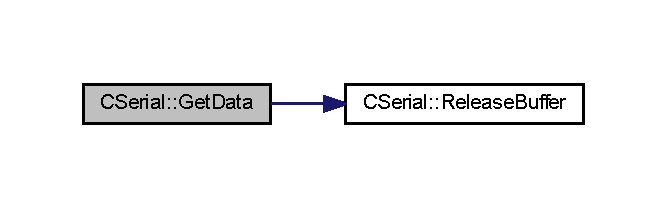
\includegraphics[width=320pt]{class_c_serial_abad86c07f530569b2ceeea75bda485ad_cgraph}
\end{center}
\end{figure}
Here is the caller graph for this function\+:\nopagebreak
\begin{figure}[H]
\begin{center}
\leavevmode
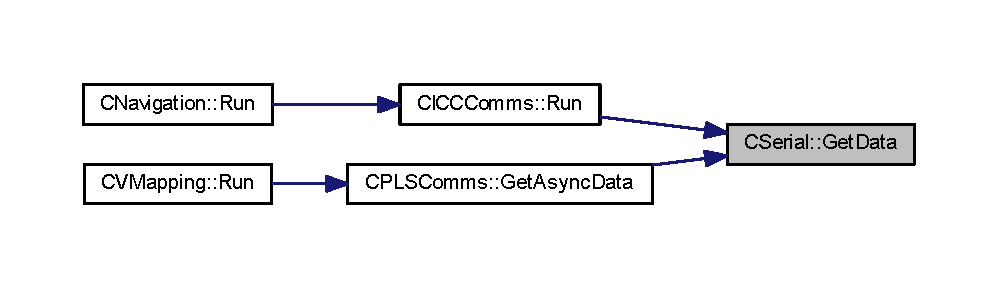
\includegraphics[width=350pt]{class_c_serial_abad86c07f530569b2ceeea75bda485ad_icgraph}
\end{center}
\end{figure}
\mbox{\Hypertarget{class_c_serial_a4327d6041fe9a390612b214709027cbb}\label{class_c_serial_a4327d6041fe9a390612b214709027cbb}} 
\index{CSerial@{CSerial}!GetDataLen@{GetDataLen}}
\index{GetDataLen@{GetDataLen}!CSerial@{CSerial}}
\subsubsection{\texorpdfstring{GetDataLen()}{GetDataLen()}}
{\footnotesize\ttfamily \mbox{\hyperlink{_a_d_a_s___types_8h_a1f1825b69244eb3ad2c7165ddc99c956}{uint16\+\_\+t}} C\+Serial\+::\+Get\+Data\+Len (\begin{DoxyParamCaption}\item[{void}]{ }\end{DoxyParamCaption})}



Function to get length of data. 

\begin{DoxyReturn}{Returns}
Returns length of data 
\end{DoxyReturn}


Definition at line 137 of file H\+A\+L\+\_\+\+Serial\+\_\+\+I\+F.\+cpp.

Here is the caller graph for this function\+:\nopagebreak
\begin{figure}[H]
\begin{center}
\leavevmode
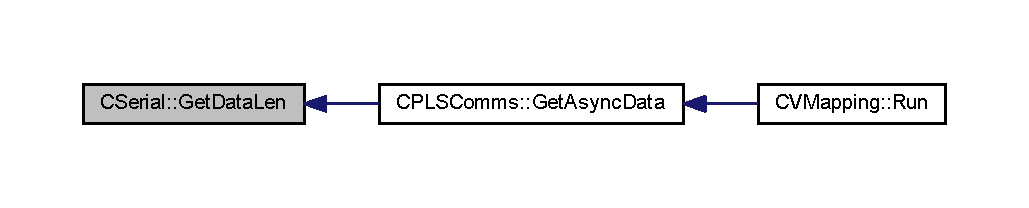
\includegraphics[width=350pt]{class_c_serial_a4327d6041fe9a390612b214709027cbb_icgraph}
\end{center}
\end{figure}
\mbox{\Hypertarget{class_c_serial_aed500bd204c4b37665d6d228333edafb}\label{class_c_serial_aed500bd204c4b37665d6d228333edafb}} 
\index{CSerial@{CSerial}!Init@{Init}}
\index{Init@{Init}!CSerial@{CSerial}}
\subsubsection{\texorpdfstring{Init()}{Init()}}
{\footnotesize\ttfamily void C\+Serial\+::\+Init (\begin{DoxyParamCaption}\item[{void}]{ }\end{DoxyParamCaption})}



Initialization function of \mbox{\hyperlink{class_c_serial}{C\+Serial}}. 



Definition at line 39 of file H\+A\+L\+\_\+\+Serial\+\_\+\+I\+F.\+cpp.

Here is the caller graph for this function\+:\nopagebreak
\begin{figure}[H]
\begin{center}
\leavevmode
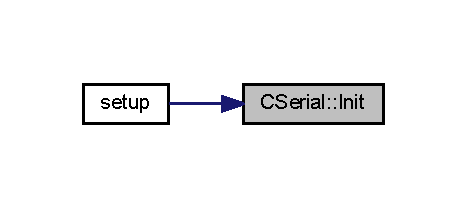
\includegraphics[width=224pt]{class_c_serial_aed500bd204c4b37665d6d228333edafb_icgraph}
\end{center}
\end{figure}
\mbox{\Hypertarget{class_c_serial_a941e5cae2ca04518925a3b32f51110a6}\label{class_c_serial_a941e5cae2ca04518925a3b32f51110a6}} 
\index{CSerial@{CSerial}!ReleaseBuffer@{ReleaseBuffer}}
\index{ReleaseBuffer@{ReleaseBuffer}!CSerial@{CSerial}}
\subsubsection{\texorpdfstring{ReleaseBuffer()}{ReleaseBuffer()}}
{\footnotesize\ttfamily void C\+Serial\+::\+Release\+Buffer (\begin{DoxyParamCaption}\item[{void}]{ }\end{DoxyParamCaption})}



Function to release buffer. 



Definition at line 161 of file H\+A\+L\+\_\+\+Serial\+\_\+\+I\+F.\+cpp.

Here is the caller graph for this function\+:\nopagebreak
\begin{figure}[H]
\begin{center}
\leavevmode
\includegraphics[width=350pt]{class_c_serial_a941e5cae2ca04518925a3b32f51110a6_icgraph}
\end{center}
\end{figure}
\mbox{\Hypertarget{class_c_serial_ae5bec6d6a1c75839ae02cf0069d1f08e}\label{class_c_serial_ae5bec6d6a1c75839ae02cf0069d1f08e}} 
\index{CSerial@{CSerial}!Send@{Send}}
\index{Send@{Send}!CSerial@{CSerial}}
\subsubsection{\texorpdfstring{Send()}{Send()}}
{\footnotesize\ttfamily bool C\+Serial\+::\+Send (\begin{DoxyParamCaption}\item[{char}]{Buff\mbox{[}$\,$\mbox{]},  }\item[{\mbox{\hyperlink{_a_d_a_s___types_8h_aba7bc1797add20fe3efdf37ced1182c5}{uint8\+\_\+t}}}]{len }\end{DoxyParamCaption})}



Function to send data in transmit buffer. 


\begin{DoxyParams}{Parameters}
{\em Buff} & Handover of transmit buffer \\
\hline
{\em len} & Length of data \\
\hline
\end{DoxyParams}
\begin{DoxyReturn}{Returns}
Returns a true if successfully sent 
\end{DoxyReturn}


Definition at line 97 of file H\+A\+L\+\_\+\+Serial\+\_\+\+I\+F.\+cpp.

\mbox{\Hypertarget{class_c_serial_a974812db5ced18cb9a6a73dc9034e7c8}\label{class_c_serial_a974812db5ced18cb9a6a73dc9034e7c8}} 
\index{CSerial@{CSerial}!SerialISRcommICC@{SerialISRcommICC}}
\index{SerialISRcommICC@{SerialISRcommICC}!CSerial@{CSerial}}
\subsubsection{\texorpdfstring{SerialISRcommICC()}{SerialISRcommICC()}}
{\footnotesize\ttfamily void C\+Serial\+::\+Serial\+I\+S\+Rcomm\+I\+CC (\begin{DoxyParamCaption}\item[{void}]{ }\end{DoxyParamCaption})}



Function for I\+SR U\+S\+A\+R\+Tn\+\_\+\+R\+X\+\_\+vect for inter-\/controller communication. 



Definition at line 215 of file H\+A\+L\+\_\+\+Serial\+\_\+\+I\+F.\+cpp.

Here is the caller graph for this function\+:
\nopagebreak
\begin{figure}[H]
\begin{center}
\leavevmode
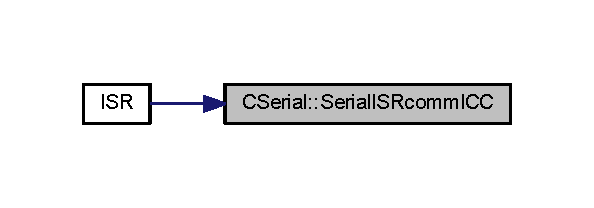
\includegraphics[width=285pt]{class_c_serial_a974812db5ced18cb9a6a73dc9034e7c8_icgraph}
\end{center}
\end{figure}
\mbox{\Hypertarget{class_c_serial_a707841754d94fc1ab6679f52bf413d85}\label{class_c_serial_a707841754d94fc1ab6679f52bf413d85}} 
\index{CSerial@{CSerial}!SerialISRcommPLS@{SerialISRcommPLS}}
\index{SerialISRcommPLS@{SerialISRcommPLS}!CSerial@{CSerial}}
\subsubsection{\texorpdfstring{SerialISRcommPLS()}{SerialISRcommPLS()}}
{\footnotesize\ttfamily void C\+Serial\+::\+Serial\+I\+S\+Rcomm\+P\+LS (\begin{DoxyParamCaption}\item[{void}]{ }\end{DoxyParamCaption})}



Function for I\+SR U\+S\+A\+R\+Tn\+\_\+\+R\+X\+\_\+vect for P\+LS communication. 



Definition at line 169 of file H\+A\+L\+\_\+\+Serial\+\_\+\+I\+F.\+cpp.

Here is the caller graph for this function\+:
\nopagebreak
\begin{figure}[H]
\begin{center}
\leavevmode
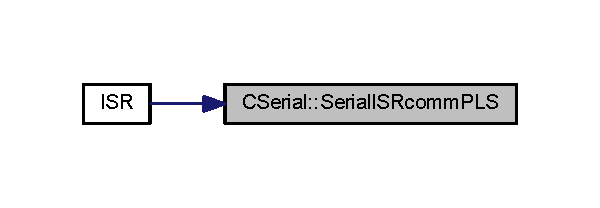
\includegraphics[width=288pt]{class_c_serial_a707841754d94fc1ab6679f52bf413d85_icgraph}
\end{center}
\end{figure}


The documentation for this class was generated from the following files\+:\begin{DoxyCompactItemize}
\item 
\mbox{\hyperlink{_h_a_l___serial___i_f_8h}{H\+A\+L\+\_\+\+Serial\+\_\+\+I\+F.\+h}}\item 
\mbox{\hyperlink{_h_a_l___serial___i_f_8cpp}{H\+A\+L\+\_\+\+Serial\+\_\+\+I\+F.\+cpp}}\end{DoxyCompactItemize}

\hypertarget{class_c_task_ctrl}{}\section{C\+Task\+Ctrl Class Reference}
\label{class_c_task_ctrl}\index{CTaskCtrl@{CTaskCtrl}}


Task scheduler class.  




{\ttfamily \#include $<$O\+S\+A\+L\+\_\+\+Task\+Ctrl.\+h$>$}



Collaboration diagram for C\+Task\+Ctrl\+:
\nopagebreak
\begin{figure}[H]
\begin{center}
\leavevmode
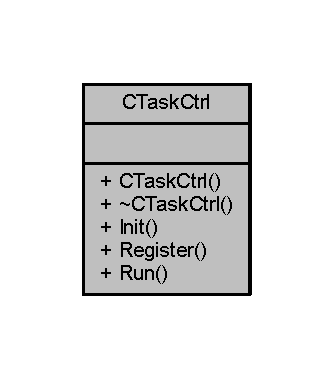
\includegraphics[width=160pt]{class_c_task_ctrl__coll__graph}
\end{center}
\end{figure}
\subsection*{Public Member Functions}
\begin{DoxyCompactItemize}
\item 
\mbox{\hyperlink{class_c_task_ctrl_a4d459479b49c5d6e1d07e9306748abe3}{C\+Task\+Ctrl}} ()
\begin{DoxyCompactList}\small\item\em Task controller class constructor. \end{DoxyCompactList}\item 
\mbox{\hyperlink{class_c_task_ctrl_a525a2b4438270d4ea5fce41e646c5b17}{$\sim$\+C\+Task\+Ctrl}} ()
\begin{DoxyCompactList}\small\item\em Task controller class destructor. \end{DoxyCompactList}\item 
void \mbox{\hyperlink{class_c_task_ctrl_a12ec6e8d4a490eba9ebdf22d32cf292b}{Init}} (void)
\begin{DoxyCompactList}\small\item\em Initialization function task controller. \end{DoxyCompactList}\item 
bool \mbox{\hyperlink{class_c_task_ctrl_a20457bd4d4a033c8aeeb44e9d4dc3c7c}{Register}} (\mbox{\hyperlink{class_i_task___i_f}{I\+Task\+\_\+\+IF}} $\ast$p\+Task, \mbox{\hyperlink{_a_d_a_s___types_8h_aba7bc1797add20fe3efdf37ced1182c5}{uint8\+\_\+t}} ID)
\begin{DoxyCompactList}\small\item\em A\+PI for registering an application. \end{DoxyCompactList}\item 
void \mbox{\hyperlink{class_c_task_ctrl_ab36ffef43b3bd33303ed7d068b2e89cf}{Run}} (void)
\begin{DoxyCompactList}\small\item\em run all task run function one by one \end{DoxyCompactList}\end{DoxyCompactItemize}


\subsection{Detailed Description}
Task scheduler class. 

implements scheduling functionality for A\+D\+AS 

Definition at line 18 of file O\+S\+A\+L\+\_\+\+Task\+Ctrl.\+h.



\subsection{Constructor \& Destructor Documentation}
\mbox{\Hypertarget{class_c_task_ctrl_a4d459479b49c5d6e1d07e9306748abe3}\label{class_c_task_ctrl_a4d459479b49c5d6e1d07e9306748abe3}} 
\index{CTaskCtrl@{CTaskCtrl}!CTaskCtrl@{CTaskCtrl}}
\index{CTaskCtrl@{CTaskCtrl}!CTaskCtrl@{CTaskCtrl}}
\subsubsection{\texorpdfstring{CTaskCtrl()}{CTaskCtrl()}}
{\footnotesize\ttfamily C\+Task\+Ctrl\+::\+C\+Task\+Ctrl (\begin{DoxyParamCaption}{ }\end{DoxyParamCaption})}



Task controller class constructor. 



Definition at line 12 of file O\+S\+A\+L\+\_\+\+Task\+Ctrl.\+cpp.

\mbox{\Hypertarget{class_c_task_ctrl_a525a2b4438270d4ea5fce41e646c5b17}\label{class_c_task_ctrl_a525a2b4438270d4ea5fce41e646c5b17}} 
\index{CTaskCtrl@{CTaskCtrl}!````~CTaskCtrl@{$\sim$CTaskCtrl}}
\index{````~CTaskCtrl@{$\sim$CTaskCtrl}!CTaskCtrl@{CTaskCtrl}}
\subsubsection{\texorpdfstring{$\sim$CTaskCtrl()}{~CTaskCtrl()}}
{\footnotesize\ttfamily C\+Task\+Ctrl\+::$\sim$\+C\+Task\+Ctrl (\begin{DoxyParamCaption}{ }\end{DoxyParamCaption})}



Task controller class destructor. 



Definition at line 18 of file O\+S\+A\+L\+\_\+\+Task\+Ctrl.\+cpp.



\subsection{Member Function Documentation}
\mbox{\Hypertarget{class_c_task_ctrl_a12ec6e8d4a490eba9ebdf22d32cf292b}\label{class_c_task_ctrl_a12ec6e8d4a490eba9ebdf22d32cf292b}} 
\index{CTaskCtrl@{CTaskCtrl}!Init@{Init}}
\index{Init@{Init}!CTaskCtrl@{CTaskCtrl}}
\subsubsection{\texorpdfstring{Init()}{Init()}}
{\footnotesize\ttfamily void C\+Task\+Ctrl\+::\+Init (\begin{DoxyParamCaption}\item[{void}]{ }\end{DoxyParamCaption})}



Initialization function task controller. 

Initialize all application. 

Definition at line 23 of file O\+S\+A\+L\+\_\+\+Task\+Ctrl.\+cpp.

Here is the call graph for this function\+:
\nopagebreak
\begin{figure}[H]
\begin{center}
\leavevmode
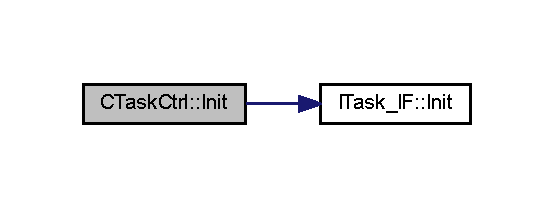
\includegraphics[width=266pt]{class_c_task_ctrl_a12ec6e8d4a490eba9ebdf22d32cf292b_cgraph}
\end{center}
\end{figure}
Here is the caller graph for this function\+:
\nopagebreak
\begin{figure}[H]
\begin{center}
\leavevmode
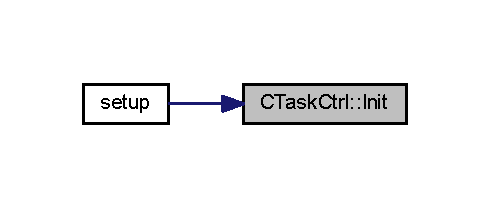
\includegraphics[width=235pt]{class_c_task_ctrl_a12ec6e8d4a490eba9ebdf22d32cf292b_icgraph}
\end{center}
\end{figure}
\mbox{\Hypertarget{class_c_task_ctrl_a20457bd4d4a033c8aeeb44e9d4dc3c7c}\label{class_c_task_ctrl_a20457bd4d4a033c8aeeb44e9d4dc3c7c}} 
\index{CTaskCtrl@{CTaskCtrl}!Register@{Register}}
\index{Register@{Register}!CTaskCtrl@{CTaskCtrl}}
\subsubsection{\texorpdfstring{Register()}{Register()}}
{\footnotesize\ttfamily bool C\+Task\+Ctrl\+::\+Register (\begin{DoxyParamCaption}\item[{\mbox{\hyperlink{class_i_task___i_f}{I\+Task\+\_\+\+IF}} $\ast$}]{p\+Task,  }\item[{\mbox{\hyperlink{_a_d_a_s___types_8h_aba7bc1797add20fe3efdf37ced1182c5}{uint8\+\_\+t}}}]{ID }\end{DoxyParamCaption})}



A\+PI for registering an application. 


\begin{DoxyParams}[1]{Parameters}
\mbox{\texttt{ in}}  & {\em p\+Task} & pointer to application \\
\hline
\mbox{\texttt{ in}}  & {\em ID} & priority\+ID of application \\
\hline
\end{DoxyParams}
\begin{DoxyReturn}{Returns}
true if successful 
\end{DoxyReturn}


Definition at line 34 of file O\+S\+A\+L\+\_\+\+Task\+Ctrl.\+cpp.

Here is the caller graph for this function\+:
\nopagebreak
\begin{figure}[H]
\begin{center}
\leavevmode
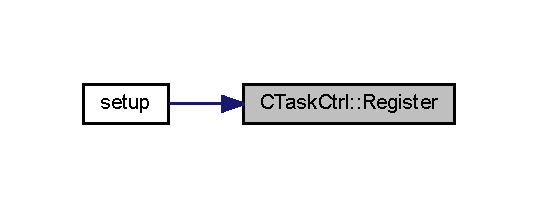
\includegraphics[width=258pt]{class_c_task_ctrl_a20457bd4d4a033c8aeeb44e9d4dc3c7c_icgraph}
\end{center}
\end{figure}
\mbox{\Hypertarget{class_c_task_ctrl_ab36ffef43b3bd33303ed7d068b2e89cf}\label{class_c_task_ctrl_ab36ffef43b3bd33303ed7d068b2e89cf}} 
\index{CTaskCtrl@{CTaskCtrl}!Run@{Run}}
\index{Run@{Run}!CTaskCtrl@{CTaskCtrl}}
\subsubsection{\texorpdfstring{Run()}{Run()}}
{\footnotesize\ttfamily void C\+Task\+Ctrl\+::\+Run (\begin{DoxyParamCaption}\item[{void}]{ }\end{DoxyParamCaption})}



run all task run function one by one 

run all run of applications one by one 

Definition at line 48 of file O\+S\+A\+L\+\_\+\+Task\+Ctrl.\+cpp.

Here is the call graph for this function\+:
\nopagebreak
\begin{figure}[H]
\begin{center}
\leavevmode
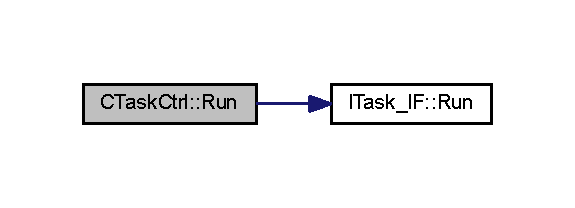
\includegraphics[width=276pt]{class_c_task_ctrl_ab36ffef43b3bd33303ed7d068b2e89cf_cgraph}
\end{center}
\end{figure}
Here is the caller graph for this function\+:
\nopagebreak
\begin{figure}[H]
\begin{center}
\leavevmode
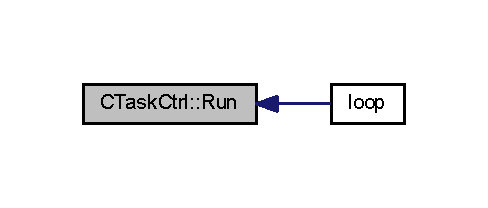
\includegraphics[width=234pt]{class_c_task_ctrl_ab36ffef43b3bd33303ed7d068b2e89cf_icgraph}
\end{center}
\end{figure}


The documentation for this class was generated from the following files\+:\begin{DoxyCompactItemize}
\item 
\mbox{\hyperlink{_o_s_a_l___task_ctrl_8h}{O\+S\+A\+L\+\_\+\+Task\+Ctrl.\+h}}\item 
\mbox{\hyperlink{_o_s_a_l___task_ctrl_8cpp}{O\+S\+A\+L\+\_\+\+Task\+Ctrl.\+cpp}}\end{DoxyCompactItemize}

\hypertarget{class_c_user___i_f}{}\section{C\+User\+\_\+\+IF Class Reference}
\label{class_c_user___i_f}\index{CUser\_IF@{CUser\_IF}}


{\ttfamily \#include $<$App\+\_\+\+User\+Interface.\+h$>$}



Inheritance diagram for C\+User\+\_\+\+IF\+:\nopagebreak
\begin{figure}[H]
\begin{center}
\leavevmode
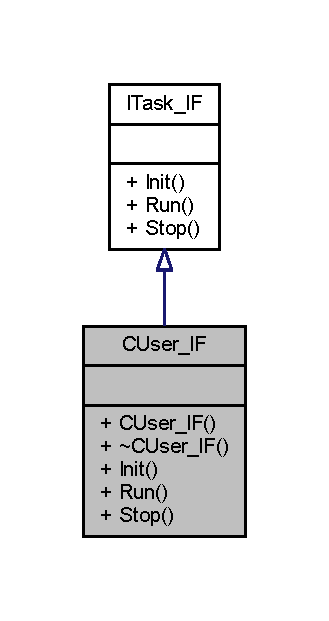
\includegraphics[width=158pt]{class_c_user___i_f__inherit__graph}
\end{center}
\end{figure}


Collaboration diagram for C\+User\+\_\+\+IF\+:\nopagebreak
\begin{figure}[H]
\begin{center}
\leavevmode
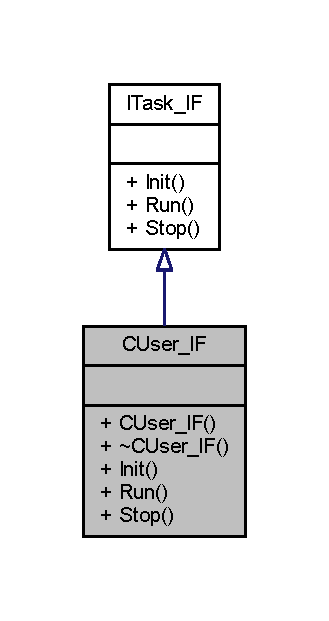
\includegraphics[width=158pt]{class_c_user___i_f__coll__graph}
\end{center}
\end{figure}
\subsection*{Public Member Functions}
\begin{DoxyCompactItemize}
\item 
\mbox{\hyperlink{class_c_user___i_f_a417b492fc7368c7d5dde59587f4b3e65}{C\+User\+\_\+\+IF}} ()
\begin{DoxyCompactList}\small\item\em user interface app class constructor. \end{DoxyCompactList}\item 
\mbox{\hyperlink{class_c_user___i_f_a35f3408f44d101a06e184311cab14cba}{$\sim$\+C\+User\+\_\+\+IF}} ()
\begin{DoxyCompactList}\small\item\em user interface app class destructor. \end{DoxyCompactList}\item 
virtual void \mbox{\hyperlink{class_c_user___i_f_a02c8bba754c77583dc5afaa6877dc547}{Init}} (void)
\begin{DoxyCompactList}\small\item\em Initialization function of user interface Application. \end{DoxyCompactList}\item 
virtual void \mbox{\hyperlink{class_c_user___i_f_a1be2e11cd5df5ad0fa5a74a0eb283ec5}{Run}} (void)
\begin{DoxyCompactList}\small\item\em Run function of user interface Application. \end{DoxyCompactList}\item 
virtual void \mbox{\hyperlink{class_c_user___i_f_ae241b3296f4dd7810897ed8631ede880}{Stop}} (void)
\begin{DoxyCompactList}\small\item\em Stop/shutdown function of user interface Application. \end{DoxyCompactList}\end{DoxyCompactItemize}


\subsection{Detailed Description}
Template class user interface contains only basic functionality required by task controller 

Definition at line 19 of file App\+\_\+\+User\+Interface.\+h.



\subsection{Constructor \& Destructor Documentation}
\mbox{\Hypertarget{class_c_user___i_f_a417b492fc7368c7d5dde59587f4b3e65}\label{class_c_user___i_f_a417b492fc7368c7d5dde59587f4b3e65}} 
\index{CUser\_IF@{CUser\_IF}!CUser\_IF@{CUser\_IF}}
\index{CUser\_IF@{CUser\_IF}!CUser\_IF@{CUser\_IF}}
\subsubsection{\texorpdfstring{CUser\_IF()}{CUser\_IF()}}
{\footnotesize\ttfamily C\+User\+\_\+\+I\+F\+::\+C\+User\+\_\+\+IF (\begin{DoxyParamCaption}{ }\end{DoxyParamCaption})}



user interface app class constructor. 



Definition at line 13 of file App\+\_\+\+User\+Interface.\+cpp.

\mbox{\Hypertarget{class_c_user___i_f_a35f3408f44d101a06e184311cab14cba}\label{class_c_user___i_f_a35f3408f44d101a06e184311cab14cba}} 
\index{CUser\_IF@{CUser\_IF}!````~CUser\_IF@{$\sim$CUser\_IF}}
\index{````~CUser\_IF@{$\sim$CUser\_IF}!CUser\_IF@{CUser\_IF}}
\subsubsection{\texorpdfstring{$\sim$CUser\_IF()}{~CUser\_IF()}}
{\footnotesize\ttfamily C\+User\+\_\+\+I\+F\+::$\sim$\+C\+User\+\_\+\+IF (\begin{DoxyParamCaption}{ }\end{DoxyParamCaption})}



user interface app class destructor. 



Definition at line 18 of file App\+\_\+\+User\+Interface.\+cpp.



\subsection{Member Function Documentation}
\mbox{\Hypertarget{class_c_user___i_f_a02c8bba754c77583dc5afaa6877dc547}\label{class_c_user___i_f_a02c8bba754c77583dc5afaa6877dc547}} 
\index{CUser\_IF@{CUser\_IF}!Init@{Init}}
\index{Init@{Init}!CUser\_IF@{CUser\_IF}}
\subsubsection{\texorpdfstring{Init()}{Init()}}
{\footnotesize\ttfamily void C\+User\+\_\+\+I\+F\+::\+Init (\begin{DoxyParamCaption}\item[{void}]{ }\end{DoxyParamCaption})\hspace{0.3cm}{\ttfamily [virtual]}}



Initialization function of user interface Application. 

Realization of pure virtual function task\+\_\+\+IF Called by task controller for initializing applications 

Implements \mbox{\hyperlink{class_i_task___i_f_a28f608bdb9b19658403f7b9b7421968d}{I\+Task\+\_\+\+IF}}.



Definition at line 22 of file App\+\_\+\+User\+Interface.\+cpp.

\mbox{\Hypertarget{class_c_user___i_f_a1be2e11cd5df5ad0fa5a74a0eb283ec5}\label{class_c_user___i_f_a1be2e11cd5df5ad0fa5a74a0eb283ec5}} 
\index{CUser\_IF@{CUser\_IF}!Run@{Run}}
\index{Run@{Run}!CUser\_IF@{CUser\_IF}}
\subsubsection{\texorpdfstring{Run()}{Run()}}
{\footnotesize\ttfamily void C\+User\+\_\+\+I\+F\+::\+Run (\begin{DoxyParamCaption}\item[{void}]{ }\end{DoxyParamCaption})\hspace{0.3cm}{\ttfamily [virtual]}}



Run function of user interface Application. 

Realization of pure virtual function task\+\_\+\+IF Called by task controller for running functionality 

Implements \mbox{\hyperlink{class_i_task___i_f_ab73cc5879a61d00fc59b72cce32cc6f7}{I\+Task\+\_\+\+IF}}.



Definition at line 27 of file App\+\_\+\+User\+Interface.\+cpp.

\mbox{\Hypertarget{class_c_user___i_f_ae241b3296f4dd7810897ed8631ede880}\label{class_c_user___i_f_ae241b3296f4dd7810897ed8631ede880}} 
\index{CUser\_IF@{CUser\_IF}!Stop@{Stop}}
\index{Stop@{Stop}!CUser\_IF@{CUser\_IF}}
\subsubsection{\texorpdfstring{Stop()}{Stop()}}
{\footnotesize\ttfamily void C\+User\+\_\+\+I\+F\+::\+Stop (\begin{DoxyParamCaption}\item[{void}]{ }\end{DoxyParamCaption})\hspace{0.3cm}{\ttfamily [virtual]}}



Stop/shutdown function of user interface Application. 

Realization of pure virtual function task\+\_\+\+IF Called by task controller for shutdown 

Implements \mbox{\hyperlink{class_i_task___i_f_af5f8fba86704c7e36d0e4681d58300c6}{I\+Task\+\_\+\+IF}}.



Definition at line 32 of file App\+\_\+\+User\+Interface.\+cpp.



The documentation for this class was generated from the following files\+:\begin{DoxyCompactItemize}
\item 
\mbox{\hyperlink{_app___user_interface_8h}{App\+\_\+\+User\+Interface.\+h}}\item 
\mbox{\hyperlink{_app___user_interface_8cpp}{App\+\_\+\+User\+Interface.\+cpp}}\end{DoxyCompactItemize}

\hypertarget{class_c_v_mapping}{}\section{C\+V\+Mapping Class Reference}
\label{class_c_v_mapping}\index{C\+V\+Mapping@{C\+V\+Mapping}}


{\ttfamily \#include $<$App\+\_\+\+Virtual\+Mapping.\+h$>$}



Inheritance diagram for C\+V\+Mapping\+:\nopagebreak
\begin{figure}[H]
\begin{center}
\leavevmode
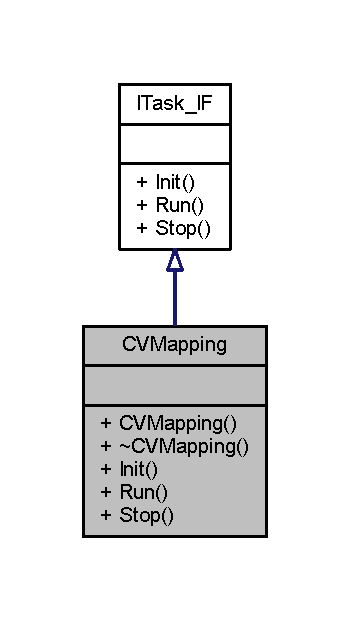
\includegraphics[width=168pt]{class_c_v_mapping__inherit__graph}
\end{center}
\end{figure}


Collaboration diagram for C\+V\+Mapping\+:\nopagebreak
\begin{figure}[H]
\begin{center}
\leavevmode
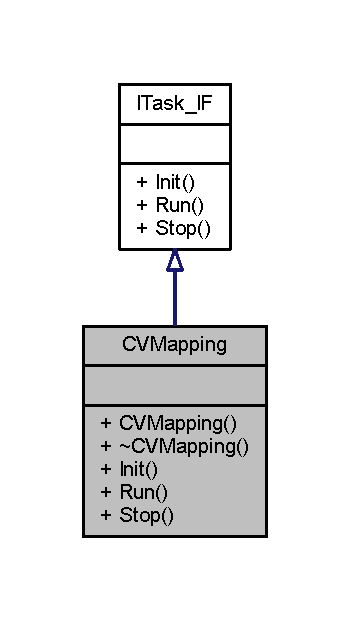
\includegraphics[width=168pt]{class_c_v_mapping__coll__graph}
\end{center}
\end{figure}
\subsection*{Public Member Functions}
\begin{DoxyCompactItemize}
\item 
\mbox{\hyperlink{class_c_v_mapping_af6ee17cb269e87c9da52a22ef29b50df}{C\+V\+Mapping}} (\mbox{\hyperlink{class_c_navigation}{C\+Navigation}} \&N\+AV, \mbox{\hyperlink{class_c_p_l_s_comms}{C\+P\+L\+S\+Comms}} \&pls\+Comms)
\item 
\mbox{\hyperlink{class_c_v_mapping_af597f7af00322fe01ec8f74838b06f08}{$\sim$\+C\+V\+Mapping}} ()
\item 
virtual void \mbox{\hyperlink{class_c_v_mapping_a110257122b8946bcb8f17051070e03eb}{Init}} (void)
\item 
virtual void \mbox{\hyperlink{class_c_v_mapping_a8f064fcfd01953d7072efd5de23f89ef}{Run}} (void)
\item 
virtual void \mbox{\hyperlink{class_c_v_mapping_ad4e34f79b444109d0cbf1223881126dc}{Stop}} (void)
\end{DoxyCompactItemize}


\subsection{Detailed Description}


Definition at line 15 of file App\+\_\+\+Virtual\+Mapping.\+h.



\subsection{Constructor \& Destructor Documentation}
\mbox{\Hypertarget{class_c_v_mapping_af6ee17cb269e87c9da52a22ef29b50df}\label{class_c_v_mapping_af6ee17cb269e87c9da52a22ef29b50df}} 
\index{C\+V\+Mapping@{C\+V\+Mapping}!C\+V\+Mapping@{C\+V\+Mapping}}
\index{C\+V\+Mapping@{C\+V\+Mapping}!C\+V\+Mapping@{C\+V\+Mapping}}
\subsubsection{\texorpdfstring{C\+V\+Mapping()}{CVMapping()}}
{\footnotesize\ttfamily C\+V\+Mapping\+::\+C\+V\+Mapping (\begin{DoxyParamCaption}\item[{\mbox{\hyperlink{class_c_navigation}{C\+Navigation}} \&}]{N\+AV,  }\item[{\mbox{\hyperlink{class_c_p_l_s_comms}{C\+P\+L\+S\+Comms}} \&}]{pls\+Comms }\end{DoxyParamCaption})}



Definition at line 60 of file App\+\_\+\+Virtual\+Mapping.\+cpp.

\mbox{\Hypertarget{class_c_v_mapping_af597f7af00322fe01ec8f74838b06f08}\label{class_c_v_mapping_af597f7af00322fe01ec8f74838b06f08}} 
\index{C\+V\+Mapping@{C\+V\+Mapping}!````~C\+V\+Mapping@{$\sim$\+C\+V\+Mapping}}
\index{````~C\+V\+Mapping@{$\sim$\+C\+V\+Mapping}!C\+V\+Mapping@{C\+V\+Mapping}}
\subsubsection{\texorpdfstring{$\sim$\+C\+V\+Mapping()}{~CVMapping()}}
{\footnotesize\ttfamily C\+V\+Mapping\+::$\sim$\+C\+V\+Mapping (\begin{DoxyParamCaption}{ }\end{DoxyParamCaption})}



Definition at line 68 of file App\+\_\+\+Virtual\+Mapping.\+cpp.



\subsection{Member Function Documentation}
\mbox{\Hypertarget{class_c_v_mapping_a110257122b8946bcb8f17051070e03eb}\label{class_c_v_mapping_a110257122b8946bcb8f17051070e03eb}} 
\index{C\+V\+Mapping@{C\+V\+Mapping}!Init@{Init}}
\index{Init@{Init}!C\+V\+Mapping@{C\+V\+Mapping}}
\subsubsection{\texorpdfstring{Init()}{Init()}}
{\footnotesize\ttfamily void C\+V\+Mapping\+::\+Init (\begin{DoxyParamCaption}\item[{void}]{ }\end{DoxyParamCaption})\hspace{0.3cm}{\ttfamily [virtual]}}



Implements \mbox{\hyperlink{class_i_task___i_f_a28f608bdb9b19658403f7b9b7421968d}{I\+Task\+\_\+\+IF}}.



Definition at line 71 of file App\+\_\+\+Virtual\+Mapping.\+cpp.

\mbox{\Hypertarget{class_c_v_mapping_a8f064fcfd01953d7072efd5de23f89ef}\label{class_c_v_mapping_a8f064fcfd01953d7072efd5de23f89ef}} 
\index{C\+V\+Mapping@{C\+V\+Mapping}!Run@{Run}}
\index{Run@{Run}!C\+V\+Mapping@{C\+V\+Mapping}}
\subsubsection{\texorpdfstring{Run()}{Run()}}
{\footnotesize\ttfamily void C\+V\+Mapping\+::\+Run (\begin{DoxyParamCaption}\item[{void}]{ }\end{DoxyParamCaption})\hspace{0.3cm}{\ttfamily [virtual]}}



Implements \mbox{\hyperlink{class_i_task___i_f_ab73cc5879a61d00fc59b72cce32cc6f7}{I\+Task\+\_\+\+IF}}.



Definition at line 76 of file App\+\_\+\+Virtual\+Mapping.\+cpp.

Here is the call graph for this function\+:\nopagebreak
\begin{figure}[H]
\begin{center}
\leavevmode
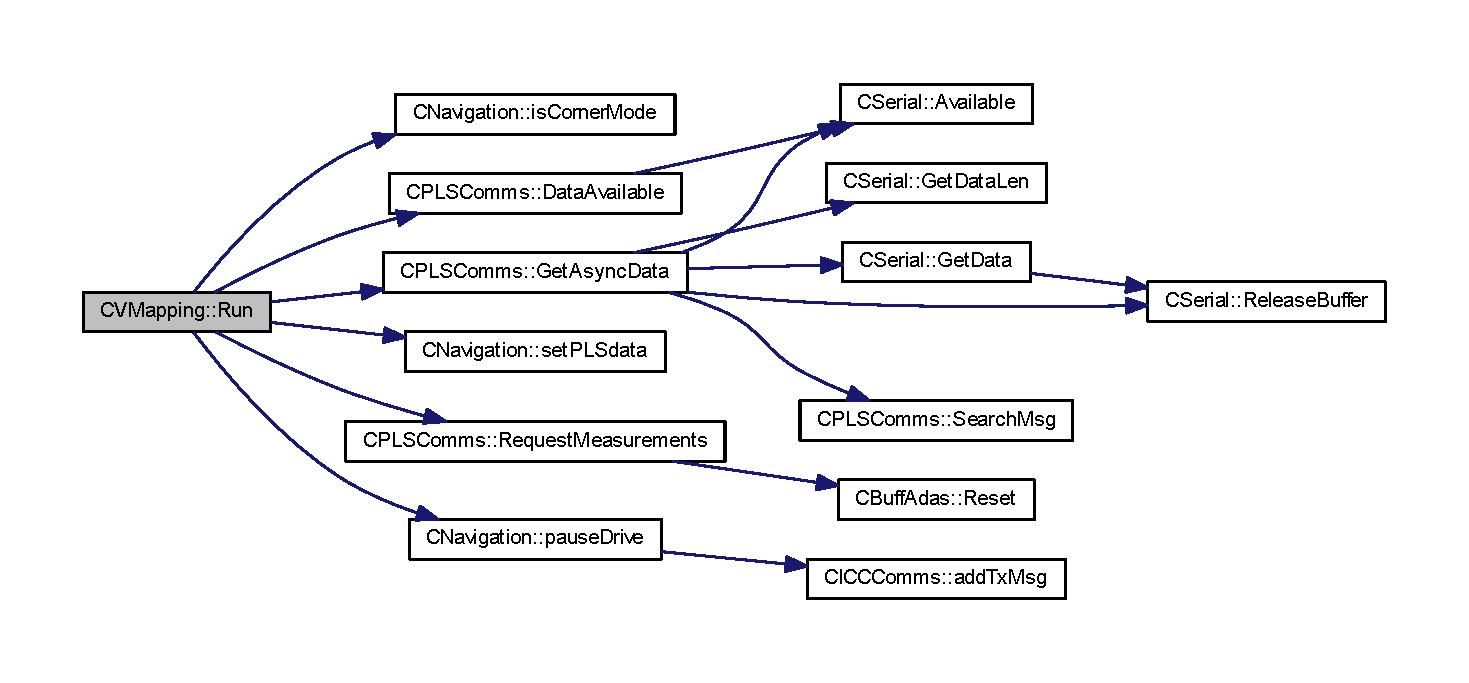
\includegraphics[width=350pt]{class_c_v_mapping_a8f064fcfd01953d7072efd5de23f89ef_cgraph}
\end{center}
\end{figure}
\mbox{\Hypertarget{class_c_v_mapping_ad4e34f79b444109d0cbf1223881126dc}\label{class_c_v_mapping_ad4e34f79b444109d0cbf1223881126dc}} 
\index{C\+V\+Mapping@{C\+V\+Mapping}!Stop@{Stop}}
\index{Stop@{Stop}!C\+V\+Mapping@{C\+V\+Mapping}}
\subsubsection{\texorpdfstring{Stop()}{Stop()}}
{\footnotesize\ttfamily void C\+V\+Mapping\+::\+Stop (\begin{DoxyParamCaption}\item[{void}]{ }\end{DoxyParamCaption})\hspace{0.3cm}{\ttfamily [virtual]}}



Implements \mbox{\hyperlink{class_i_task___i_f_af5f8fba86704c7e36d0e4681d58300c6}{I\+Task\+\_\+\+IF}}.



Definition at line 149 of file App\+\_\+\+Virtual\+Mapping.\+cpp.



The documentation for this class was generated from the following files\+:\begin{DoxyCompactItemize}
\item 
\mbox{\hyperlink{_app___virtual_mapping_8h}{App\+\_\+\+Virtual\+Mapping.\+h}}\item 
\mbox{\hyperlink{_app___virtual_mapping_8cpp}{App\+\_\+\+Virtual\+Mapping.\+cpp}}\end{DoxyCompactItemize}

\hypertarget{class_i_task___i_f}{}\section{I\+Task\+\_\+\+IF Class Reference}
\label{class_i_task___i_f}\index{I\+Task\+\_\+\+IF@{I\+Task\+\_\+\+IF}}


{\ttfamily \#include $<$Task\+\_\+\+I\+F.\+h$>$}



Inheritance diagram for I\+Task\+\_\+\+IF\+:
\nopagebreak
\begin{figure}[H]
\begin{center}
\leavevmode
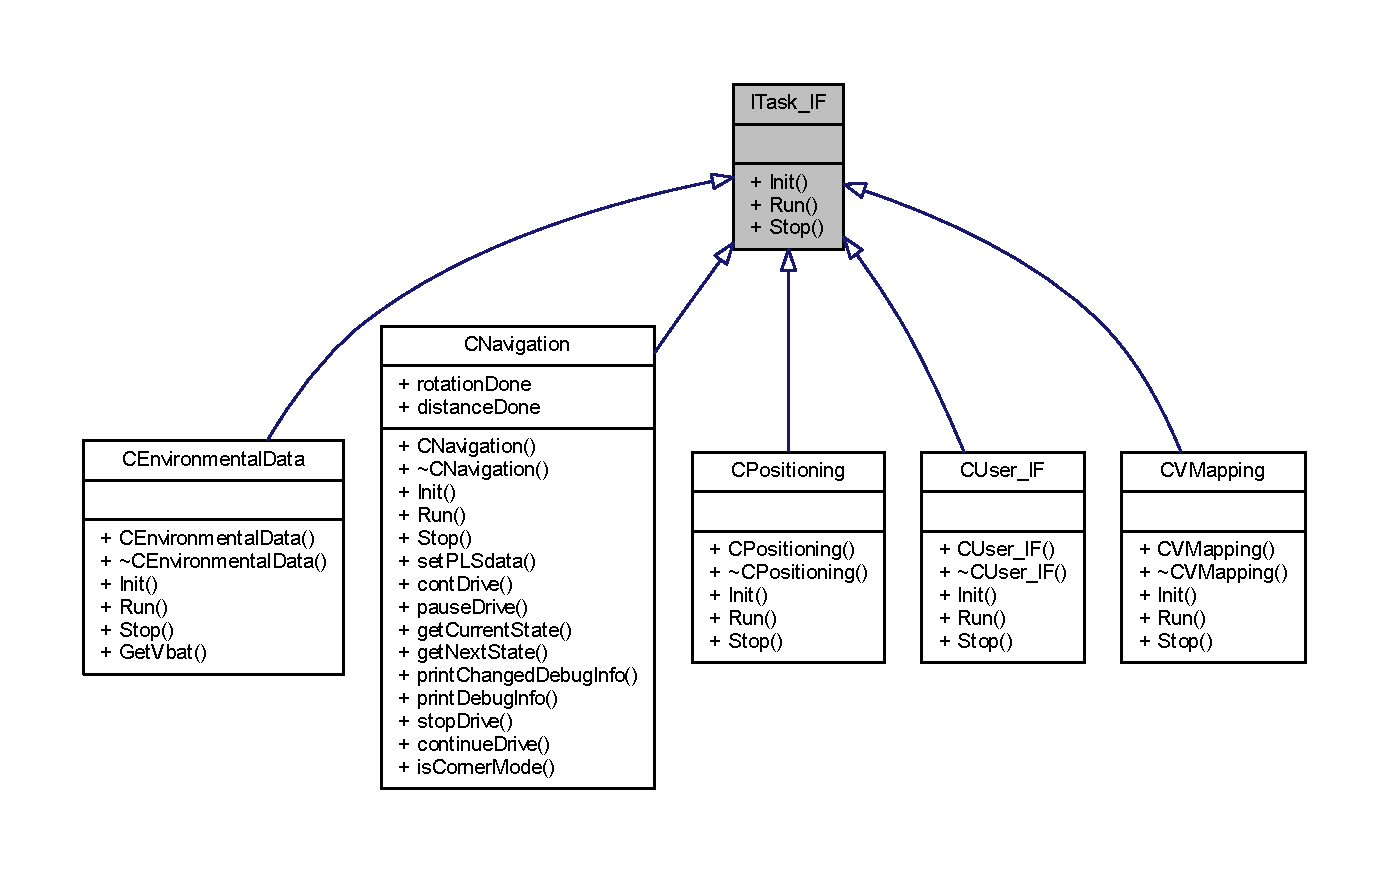
\includegraphics[width=350pt]{class_i_task___i_f__inherit__graph}
\end{center}
\end{figure}


Collaboration diagram for I\+Task\+\_\+\+IF\+:\nopagebreak
\begin{figure}[H]
\begin{center}
\leavevmode
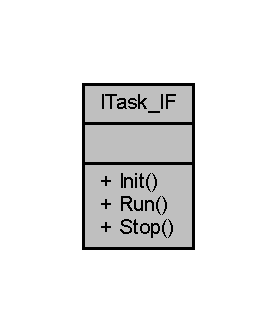
\includegraphics[width=133pt]{class_i_task___i_f__coll__graph}
\end{center}
\end{figure}
\subsection*{Public Member Functions}
\begin{DoxyCompactItemize}
\item 
virtual void \mbox{\hyperlink{class_i_task___i_f_a28f608bdb9b19658403f7b9b7421968d}{Init}} (void)=0
\item 
virtual void \mbox{\hyperlink{class_i_task___i_f_ab73cc5879a61d00fc59b72cce32cc6f7}{Run}} (void)=0
\item 
virtual void \mbox{\hyperlink{class_i_task___i_f_af5f8fba86704c7e36d0e4681d58300c6}{Stop}} (void)=0
\end{DoxyCompactItemize}


\subsection{Detailed Description}


Definition at line 12 of file Task\+\_\+\+I\+F.\+h.



\subsection{Member Function Documentation}
\mbox{\Hypertarget{class_i_task___i_f_a28f608bdb9b19658403f7b9b7421968d}\label{class_i_task___i_f_a28f608bdb9b19658403f7b9b7421968d}} 
\index{I\+Task\+\_\+\+IF@{I\+Task\+\_\+\+IF}!Init@{Init}}
\index{Init@{Init}!I\+Task\+\_\+\+IF@{I\+Task\+\_\+\+IF}}
\subsubsection{\texorpdfstring{Init()}{Init()}}
{\footnotesize\ttfamily virtual void I\+Task\+\_\+\+I\+F\+::\+Init (\begin{DoxyParamCaption}\item[{void}]{ }\end{DoxyParamCaption})\hspace{0.3cm}{\ttfamily [pure virtual]}}



Implemented in \mbox{\hyperlink{class_c_navigation_a86a0756663ccf76e9c474764b8f7a04f}{C\+Navigation}}, \mbox{\hyperlink{class_c_environmental_data_a3321cce122ef1e1f7e995ee51353e87d}{C\+Environmental\+Data}}, \mbox{\hyperlink{class_c_v_mapping_a110257122b8946bcb8f17051070e03eb}{C\+V\+Mapping}}, \mbox{\hyperlink{class_c_positioning_abdceba66e701554a178acf61c61b0df6}{C\+Positioning}}, and \mbox{\hyperlink{class_c_user___i_f_a02c8bba754c77583dc5afaa6877dc547}{C\+User\+\_\+\+IF}}.

Here is the caller graph for this function\+:\nopagebreak
\begin{figure}[H]
\begin{center}
\leavevmode
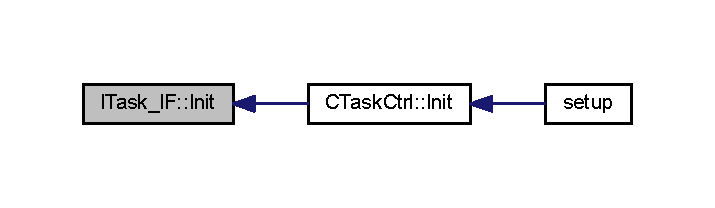
\includegraphics[width=343pt]{class_i_task___i_f_a28f608bdb9b19658403f7b9b7421968d_icgraph}
\end{center}
\end{figure}
\mbox{\Hypertarget{class_i_task___i_f_ab73cc5879a61d00fc59b72cce32cc6f7}\label{class_i_task___i_f_ab73cc5879a61d00fc59b72cce32cc6f7}} 
\index{I\+Task\+\_\+\+IF@{I\+Task\+\_\+\+IF}!Run@{Run}}
\index{Run@{Run}!I\+Task\+\_\+\+IF@{I\+Task\+\_\+\+IF}}
\subsubsection{\texorpdfstring{Run()}{Run()}}
{\footnotesize\ttfamily virtual void I\+Task\+\_\+\+I\+F\+::\+Run (\begin{DoxyParamCaption}\item[{void}]{ }\end{DoxyParamCaption})\hspace{0.3cm}{\ttfamily [pure virtual]}}



Implemented in \mbox{\hyperlink{class_c_navigation_a86acb1521aab400e542465c8eabed671}{C\+Navigation}}, \mbox{\hyperlink{class_c_environmental_data_a586a729d3aab2873812517d950c91242}{C\+Environmental\+Data}}, \mbox{\hyperlink{class_c_v_mapping_a8f064fcfd01953d7072efd5de23f89ef}{C\+V\+Mapping}}, \mbox{\hyperlink{class_c_positioning_ad0e439dcc95c450548c2806077aeff57}{C\+Positioning}}, and \mbox{\hyperlink{class_c_user___i_f_a1be2e11cd5df5ad0fa5a74a0eb283ec5}{C\+User\+\_\+\+IF}}.

Here is the caller graph for this function\+:\nopagebreak
\begin{figure}[H]
\begin{center}
\leavevmode
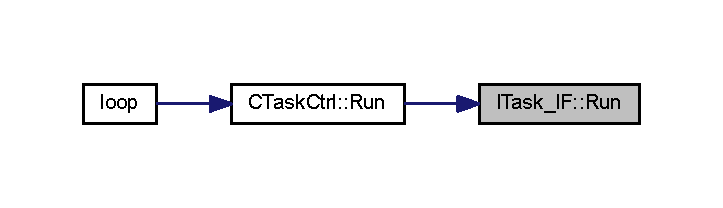
\includegraphics[width=347pt]{class_i_task___i_f_ab73cc5879a61d00fc59b72cce32cc6f7_icgraph}
\end{center}
\end{figure}
\mbox{\Hypertarget{class_i_task___i_f_af5f8fba86704c7e36d0e4681d58300c6}\label{class_i_task___i_f_af5f8fba86704c7e36d0e4681d58300c6}} 
\index{I\+Task\+\_\+\+IF@{I\+Task\+\_\+\+IF}!Stop@{Stop}}
\index{Stop@{Stop}!I\+Task\+\_\+\+IF@{I\+Task\+\_\+\+IF}}
\subsubsection{\texorpdfstring{Stop()}{Stop()}}
{\footnotesize\ttfamily virtual void I\+Task\+\_\+\+I\+F\+::\+Stop (\begin{DoxyParamCaption}\item[{void}]{ }\end{DoxyParamCaption})\hspace{0.3cm}{\ttfamily [pure virtual]}}



Implemented in \mbox{\hyperlink{class_c_navigation_a3cc8f7fdd003d6b2c5056b87ff93edd9}{C\+Navigation}}, \mbox{\hyperlink{class_c_environmental_data_a61a8f487f013602aab4dadcf8a9da4c8}{C\+Environmental\+Data}}, \mbox{\hyperlink{class_c_v_mapping_ad4e34f79b444109d0cbf1223881126dc}{C\+V\+Mapping}}, \mbox{\hyperlink{class_c_positioning_a2706c9bb6bb52201c279386fd2c9dd89}{C\+Positioning}}, and \mbox{\hyperlink{class_c_user___i_f_ae241b3296f4dd7810897ed8631ede880}{C\+User\+\_\+\+IF}}.



The documentation for this class was generated from the following file\+:\begin{DoxyCompactItemize}
\item 
\mbox{\hyperlink{_task___i_f_8h}{Task\+\_\+\+I\+F.\+h}}\end{DoxyCompactItemize}

\hypertarget{struct_c_i_c_c_comms_1_1_message__t}{}\section{C\+I\+C\+C\+Comms\+::Message\+\_\+t Struct Reference}
\label{struct_c_i_c_c_comms_1_1_message__t}\index{CICCComms::Message\_t@{CICCComms::Message\_t}}


Structure for I\+CC messages.  




{\ttfamily \#include $<$Comm\+\_\+\+I\+C\+C.\+h$>$}



Collaboration diagram for C\+I\+C\+C\+Comms\+::Message\+\_\+t\+:
\nopagebreak
\begin{figure}[H]
\begin{center}
\leavevmode
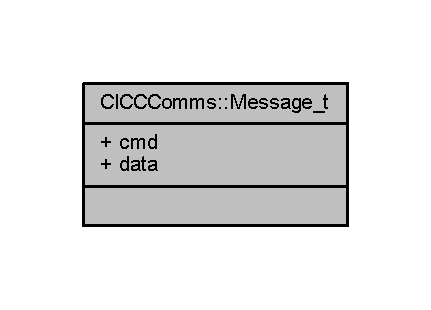
\includegraphics[width=207pt]{struct_c_i_c_c_comms_1_1_message__t__coll__graph}
\end{center}
\end{figure}
\subsection*{Public Attributes}
\begin{DoxyCompactItemize}
\item 
\mbox{\hyperlink{_a_d_a_s___types_8h_aba7bc1797add20fe3efdf37ced1182c5}{uint8\+\_\+t}} \mbox{\hyperlink{struct_c_i_c_c_comms_1_1_message__t_adf3e3290f54ee3997bc837463a340d05}{cmd}}
\item 
signed int \mbox{\hyperlink{struct_c_i_c_c_comms_1_1_message__t_a25cfce11e78d103524b695b281629d75}{data}}
\end{DoxyCompactItemize}


\subsection{Detailed Description}
Structure for I\+CC messages. 

Definition at line 26 of file Comm\+\_\+\+I\+C\+C.\+h.



\subsection{Member Data Documentation}
\mbox{\Hypertarget{struct_c_i_c_c_comms_1_1_message__t_adf3e3290f54ee3997bc837463a340d05}\label{struct_c_i_c_c_comms_1_1_message__t_adf3e3290f54ee3997bc837463a340d05}} 
\index{CICCComms::Message\_t@{CICCComms::Message\_t}!cmd@{cmd}}
\index{cmd@{cmd}!CICCComms::Message\_t@{CICCComms::Message\_t}}
\subsubsection{\texorpdfstring{cmd}{cmd}}
{\footnotesize\ttfamily \mbox{\hyperlink{_a_d_a_s___types_8h_aba7bc1797add20fe3efdf37ced1182c5}{uint8\+\_\+t}} C\+I\+C\+C\+Comms\+::\+Message\+\_\+t\+::cmd}

Command as uint8\+\_\+t 

Definition at line 27 of file Comm\+\_\+\+I\+C\+C.\+h.

\mbox{\Hypertarget{struct_c_i_c_c_comms_1_1_message__t_a25cfce11e78d103524b695b281629d75}\label{struct_c_i_c_c_comms_1_1_message__t_a25cfce11e78d103524b695b281629d75}} 
\index{CICCComms::Message\_t@{CICCComms::Message\_t}!data@{data}}
\index{data@{data}!CICCComms::Message\_t@{CICCComms::Message\_t}}
\subsubsection{\texorpdfstring{data}{data}}
{\footnotesize\ttfamily signed int C\+I\+C\+C\+Comms\+::\+Message\+\_\+t\+::data}

Data as signed int 

Definition at line 28 of file Comm\+\_\+\+I\+C\+C.\+h.



The documentation for this struct was generated from the following file\+:\begin{DoxyCompactItemize}
\item 
\mbox{\hyperlink{_comm___i_c_c_8h}{Comm\+\_\+\+I\+C\+C.\+h}}\end{DoxyCompactItemize}

\hypertarget{struct_c_p_l_s_comms_1_1_message__t}{}\section{C\+P\+L\+S\+Comms\+:\+:Message\+\_\+t Struct Reference}
\label{struct_c_p_l_s_comms_1_1_message__t}\index{C\+P\+L\+S\+Comms\+::\+Message\+\_\+t@{C\+P\+L\+S\+Comms\+::\+Message\+\_\+t}}


{\ttfamily \#include $<$Comm\+\_\+\+P\+L\+S.\+h$>$}



Collaboration diagram for C\+P\+L\+S\+Comms\+:\+:Message\+\_\+t\+:\nopagebreak
\begin{figure}[H]
\begin{center}
\leavevmode
\includegraphics[width=210pt]{struct_c_p_l_s_comms_1_1_message__t__coll__graph}
\end{center}
\end{figure}
\subsection*{Public Attributes}
\begin{DoxyCompactItemize}
\item 
\mbox{\hyperlink{_a_d_a_s___types_8h_aba7bc1797add20fe3efdf37ced1182c5}{uint8\+\_\+t}} $\ast$ \mbox{\hyperlink{struct_c_p_l_s_comms_1_1_message__t_a75d42db0cfdf64c0fe1ed1e8b0c472ed}{data}}
\item 
\mbox{\hyperlink{_a_d_a_s___types_8h_a1f1825b69244eb3ad2c7165ddc99c956}{uint16\+\_\+t}} \mbox{\hyperlink{struct_c_p_l_s_comms_1_1_message__t_a3af5b7fed96b157285ec6c8168b64276}{len}}
\item 
\mbox{\hyperlink{_a_d_a_s___types_8h_a1f1825b69244eb3ad2c7165ddc99c956}{uint16\+\_\+t}} \mbox{\hyperlink{struct_c_p_l_s_comms_1_1_message__t_a760e6f39adfed2b0440477560654f02f}{start}}
\item 
\mbox{\hyperlink{_a_d_a_s___types_8h_aba7bc1797add20fe3efdf37ced1182c5}{uint8\+\_\+t}} \mbox{\hyperlink{struct_c_p_l_s_comms_1_1_message__t_a451cdd914ba11c33528a4761ad38faee}{message\+ID}}
\end{DoxyCompactItemize}


\subsection{Detailed Description}


Definition at line 27 of file Comm\+\_\+\+P\+L\+S.\+h.



\subsection{Member Data Documentation}
\mbox{\Hypertarget{struct_c_p_l_s_comms_1_1_message__t_a75d42db0cfdf64c0fe1ed1e8b0c472ed}\label{struct_c_p_l_s_comms_1_1_message__t_a75d42db0cfdf64c0fe1ed1e8b0c472ed}} 
\index{C\+P\+L\+S\+Comms\+::\+Message\+\_\+t@{C\+P\+L\+S\+Comms\+::\+Message\+\_\+t}!data@{data}}
\index{data@{data}!C\+P\+L\+S\+Comms\+::\+Message\+\_\+t@{C\+P\+L\+S\+Comms\+::\+Message\+\_\+t}}
\subsubsection{\texorpdfstring{data}{data}}
{\footnotesize\ttfamily \mbox{\hyperlink{_a_d_a_s___types_8h_aba7bc1797add20fe3efdf37ced1182c5}{uint8\+\_\+t}}$\ast$ C\+P\+L\+S\+Comms\+::\+Message\+\_\+t\+::data}



Definition at line 28 of file Comm\+\_\+\+P\+L\+S.\+h.

\mbox{\Hypertarget{struct_c_p_l_s_comms_1_1_message__t_a3af5b7fed96b157285ec6c8168b64276}\label{struct_c_p_l_s_comms_1_1_message__t_a3af5b7fed96b157285ec6c8168b64276}} 
\index{C\+P\+L\+S\+Comms\+::\+Message\+\_\+t@{C\+P\+L\+S\+Comms\+::\+Message\+\_\+t}!len@{len}}
\index{len@{len}!C\+P\+L\+S\+Comms\+::\+Message\+\_\+t@{C\+P\+L\+S\+Comms\+::\+Message\+\_\+t}}
\subsubsection{\texorpdfstring{len}{len}}
{\footnotesize\ttfamily \mbox{\hyperlink{_a_d_a_s___types_8h_a1f1825b69244eb3ad2c7165ddc99c956}{uint16\+\_\+t}} C\+P\+L\+S\+Comms\+::\+Message\+\_\+t\+::len}



Definition at line 29 of file Comm\+\_\+\+P\+L\+S.\+h.

\mbox{\Hypertarget{struct_c_p_l_s_comms_1_1_message__t_a451cdd914ba11c33528a4761ad38faee}\label{struct_c_p_l_s_comms_1_1_message__t_a451cdd914ba11c33528a4761ad38faee}} 
\index{C\+P\+L\+S\+Comms\+::\+Message\+\_\+t@{C\+P\+L\+S\+Comms\+::\+Message\+\_\+t}!message\+ID@{message\+ID}}
\index{message\+ID@{message\+ID}!C\+P\+L\+S\+Comms\+::\+Message\+\_\+t@{C\+P\+L\+S\+Comms\+::\+Message\+\_\+t}}
\subsubsection{\texorpdfstring{message\+ID}{messageID}}
{\footnotesize\ttfamily \mbox{\hyperlink{_a_d_a_s___types_8h_aba7bc1797add20fe3efdf37ced1182c5}{uint8\+\_\+t}} C\+P\+L\+S\+Comms\+::\+Message\+\_\+t\+::message\+ID}



Definition at line 31 of file Comm\+\_\+\+P\+L\+S.\+h.

\mbox{\Hypertarget{struct_c_p_l_s_comms_1_1_message__t_a760e6f39adfed2b0440477560654f02f}\label{struct_c_p_l_s_comms_1_1_message__t_a760e6f39adfed2b0440477560654f02f}} 
\index{C\+P\+L\+S\+Comms\+::\+Message\+\_\+t@{C\+P\+L\+S\+Comms\+::\+Message\+\_\+t}!start@{start}}
\index{start@{start}!C\+P\+L\+S\+Comms\+::\+Message\+\_\+t@{C\+P\+L\+S\+Comms\+::\+Message\+\_\+t}}
\subsubsection{\texorpdfstring{start}{start}}
{\footnotesize\ttfamily \mbox{\hyperlink{_a_d_a_s___types_8h_a1f1825b69244eb3ad2c7165ddc99c956}{uint16\+\_\+t}} C\+P\+L\+S\+Comms\+::\+Message\+\_\+t\+::start}



Definition at line 30 of file Comm\+\_\+\+P\+L\+S.\+h.



The documentation for this struct was generated from the following file\+:\begin{DoxyCompactItemize}
\item 
\mbox{\hyperlink{_comm___p_l_s_8h}{Comm\+\_\+\+P\+L\+S.\+h}}\end{DoxyCompactItemize}

\chapter{File Documentation}
\hypertarget{_a_d_a_s___cfg_8h}{}\section{A\+D\+A\+S\+\_\+\+Cfg.\+h File Reference}
\label{_a_d_a_s___cfg_8h}\index{A\+D\+A\+S\+\_\+\+Cfg.\+h@{A\+D\+A\+S\+\_\+\+Cfg.\+h}}


This file contains the configuration of the vehicle.  


This graph shows which files directly or indirectly include this file\+:
\nopagebreak
\begin{figure}[H]
\begin{center}
\leavevmode
\includegraphics[width=350pt]{_a_d_a_s___cfg_8h__dep__incl}
\end{center}
\end{figure}
\subsection*{Macros}
\begin{DoxyCompactItemize}
\item 
\#define \mbox{\hyperlink{_a_d_a_s___cfg_8h_af1b7294cc1d532b3a1ab577b76852a39}{A\+D\+A\+S\+\_\+\+D\+E\+B\+U\+G2}}
\item 
\#define \mbox{\hyperlink{_a_d_a_s___cfg_8h_a00f72db64cf681b08d61977df126ec76}{P\+L\+S\+\_\+\+R\+C\+V\+\_\+\+B\+U\+F\+F\+\_\+\+S\+I\+ZE}}~500U
\item 
\#define \mbox{\hyperlink{_a_d_a_s___cfg_8h_ae3bd6bba60bc1008c82fe66f80428908}{P\+L\+S\+\_\+\+S\+N\+D\+\_\+\+B\+U\+F\+F\+\_\+\+S\+I\+ZE}}~50U
\item 
\#define \mbox{\hyperlink{_a_d_a_s___cfg_8h_abf41bed56ee0b2a8858687c4420bb110}{I\+C\+C\+\_\+\+R\+C\+V\+\_\+\+B\+U\+F\+F\+\_\+\+S\+I\+ZE}}~\mbox{\hyperlink{_a_d_a_s___cfg_8h_a17a000e80a2ce1e3be945f5484ff3dd7}{I\+C\+C\+\_\+\+L\+EN}}
\item 
\#define \mbox{\hyperlink{_a_d_a_s___cfg_8h_a5affc93ec51434d8a95645b2e3928148}{I\+C\+C\+\_\+\+S\+N\+D\+\_\+\+B\+U\+F\+F\+\_\+\+S\+I\+ZE}}~\mbox{\hyperlink{_a_d_a_s___cfg_8h_a17a000e80a2ce1e3be945f5484ff3dd7}{I\+C\+C\+\_\+\+L\+EN}}$\ast$10
\item 
\#define \mbox{\hyperlink{_a_d_a_s___cfg_8h_a4b4b233b2211ae3acf6ecf7c41f8acbb}{M\+A\+X\+\_\+\+N\+U\+M\+\_\+\+T\+A\+SK}}~5U
\item 
\#define \mbox{\hyperlink{_a_d_a_s___cfg_8h_a5ddc3cfb86290bdf3c976fc1ce56fa47}{S\+E\+R\+I\+A\+L1\+\_\+\+B\+A\+UD}}~9600
\item 
\#define \mbox{\hyperlink{_a_d_a_s___cfg_8h_ab7c4f69dae56ab78e8fb4e2c81701e77}{S\+E\+R\+I\+A\+L1\+\_\+\+B\+A\+U\+D\+\_\+\+P\+R\+E\+S\+C\+A\+LE}}~(((F\+\_\+\+C\+PU / (\mbox{\hyperlink{_a_d_a_s___cfg_8h_a5ddc3cfb86290bdf3c976fc1ce56fa47}{S\+E\+R\+I\+A\+L1\+\_\+\+B\+A\+UD}} $\ast$ 16\+U\+L))) -\/ 1)
\item 
\#define \mbox{\hyperlink{_a_d_a_s___cfg_8h_a62d0cbd008700f38d8a4fdd9aec2c554}{S\+E\+R\+I\+A\+L2\+\_\+\+B\+A\+UD}}~9600
\item 
\#define \mbox{\hyperlink{_a_d_a_s___cfg_8h_aaac720d7fe05f2b696f15ea9b2b56c7d}{S\+E\+R\+I\+A\+L2\+\_\+\+B\+A\+U\+D\+\_\+\+P\+R\+E\+S\+C\+A\+LE}}~(((F\+\_\+\+C\+PU / (\mbox{\hyperlink{_a_d_a_s___cfg_8h_a62d0cbd008700f38d8a4fdd9aec2c554}{S\+E\+R\+I\+A\+L2\+\_\+\+B\+A\+UD}} $\ast$ 16\+U\+L))) -\/ 1)
\item 
\#define \mbox{\hyperlink{_a_d_a_s___cfg_8h_aaf1f5bdadcf76f17d3f715fbbb78d567}{P\+L\+S\+\_\+\+W\+F\+\_\+\+S\+E\+G\+E\+M\+E\+N\+T\+S\+\_\+\+R\+I\+G\+HT}}~63U
\item 
\#define \mbox{\hyperlink{_a_d_a_s___cfg_8h_ad07418028b07fac4b1a3a2cc8a01a74e}{P\+L\+S\+\_\+\+W\+F\+\_\+\+S\+E\+G\+E\+M\+E\+N\+T\+S\+\_\+\+L\+E\+F\+T\+\_\+\+C\+O\+R\+N\+ER}}~117U
\item 
\#define \mbox{\hyperlink{_a_d_a_s___cfg_8h_a56c71db74384511c149652d598bf1795}{P\+L\+S\+\_\+\+W\+A\+L\+L\+\_\+\+D\+E\+T\+E\+C\+T\+I\+O\+N\+\_\+2\+\_\+\+P\+O\+I\+NT}}~45U
\item 
\#define \mbox{\hyperlink{_a_d_a_s___cfg_8h_a47e1f95a0e565aaa08112811fe539950}{P\+L\+S\+\_\+\+M\+A\+X\+\_\+\+V\+E\+R\+T\+I\+C\+A\+L\+\_\+\+D\+I\+ST}}~100U
\item 
\#define \mbox{\hyperlink{_a_d_a_s___cfg_8h_acca40b422775f8a03cd98a2e4326d906}{P\+L\+S\+\_\+\+R\+I\+G\+H\+T\+\_\+\+O\+F\+F\+S\+E\+T\+\_\+\+T\+O\+L\+E\+R\+A\+N\+CE}}~5U
\item 
\#define \mbox{\hyperlink{_a_d_a_s___cfg_8h_aedea30baea3703d1140bb971f7d1de8a}{P\+L\+S\+\_\+\+W\+F\+\_\+\+S\+E\+G\+E\+M\+E\+N\+T\+S\+\_\+\+M\+AX}}~180U
\item 
\#define \mbox{\hyperlink{_a_d_a_s___cfg_8h_a8c52736558ce47242a7c679123df76a0}{S\+I\+C\+K\+\_\+\+S\+TX}}~0x02
\item 
\#define \mbox{\hyperlink{_a_d_a_s___cfg_8h_a4ae91f90fd4b33d0bc454db3d90cf700}{S\+I\+C\+K\+\_\+\+D\+E\+S\+TR}}~0x80
\item 
\#define \mbox{\hyperlink{_a_d_a_s___cfg_8h_aa170bc1a99d2c608d5508e9b66566695}{S\+I\+C\+K\+\_\+\+A\+CK}}~0x06
\item 
\#define \mbox{\hyperlink{_a_d_a_s___cfg_8h_a6e34ca003e6bdfd81d05bcb8ea3c5eb2}{S\+I\+C\+K\+\_\+\+N\+AK}}~0x15
\item 
\#define \mbox{\hyperlink{_a_d_a_s___cfg_8h_ad9c869803f9fc9e3ffc9e962c19f028d}{P\+I\+N\+\_\+\+V\+B\+AT}}~A0
\item 
\#define \mbox{\hyperlink{_a_d_a_s___cfg_8h_a403f98f6cd7185fbd3da8bebe3406b98}{N\+A\+V\+\_\+\+S\+E\+T\+\_\+\+O\+F\+F\+S\+ET}}~80
\item 
\#define \mbox{\hyperlink{_a_d_a_s___cfg_8h_a3418793fa8fb8fe470c736d2c277e8fb}{N\+A\+V\+\_\+\+T\+O\+L\+\_\+\+O\+F\+F\+S\+ET}}~5
\item 
\#define \mbox{\hyperlink{_a_d_a_s___cfg_8h_a7ae3d3ce8d10e859369508ecb496ac07}{N\+A\+V\+\_\+\+T\+O\+L\+\_\+\+A\+N\+G\+L\+E\+\_\+\+D\+R\+I\+VE}}~5
\item 
\#define \mbox{\hyperlink{_a_d_a_s___cfg_8h_ad37cb9fe48a2b3eef8b01ec7c25d2dfc}{I\+C\+C\+\_\+\+S\+T\+X1}}~0xff
\item 
\#define \mbox{\hyperlink{_a_d_a_s___cfg_8h_a68e8b24c1a01472ef62c60e9d934f63c}{I\+C\+C\+\_\+\+S\+T\+X2}}~0xff
\item 
\#define \mbox{\hyperlink{_a_d_a_s___cfg_8h_ac9943f1124269cb02f9317d42991c503}{I\+C\+C\+\_\+\+T\+TX}}~0xee
\item 
\#define \mbox{\hyperlink{_a_d_a_s___cfg_8h_a17a000e80a2ce1e3be945f5484ff3dd7}{I\+C\+C\+\_\+\+L\+EN}}~6U
\item 
\#define \mbox{\hyperlink{_a_d_a_s___cfg_8h_a40d2abfed1ddd75059dcf6cb22827768}{I\+C\+C\+\_\+\+C\+M\+D\+\_\+\+C\+O\+N\+T\+\_\+\+D\+R\+I\+V\+E\+\_\+\+IN}}~0x01
\item 
\#define \mbox{\hyperlink{_a_d_a_s___cfg_8h_aedeacd8d3824162ab6e36fb5daf98a63}{I\+C\+C\+\_\+\+C\+M\+D\+\_\+\+E\+M\+E\+R\+\_\+\+S\+T\+OP}}~0x02
\item 
\#define \mbox{\hyperlink{_a_d_a_s___cfg_8h_a6b04b7f091aca78258644ae59974760b}{I\+C\+C\+\_\+\+C\+M\+D\+\_\+\+S\+O\+F\+T\+\_\+\+S\+T\+OP}}~0x03
\item 
\#define \mbox{\hyperlink{_a_d_a_s___cfg_8h_afdd598eb4bc8932a5361cad0bda4ce8b}{I\+C\+C\+\_\+\+C\+M\+D\+\_\+\+D\+R\+I\+V\+E\+\_\+\+D\+I\+ST}}~0x04
\item 
\#define \mbox{\hyperlink{_a_d_a_s___cfg_8h_a959554139978e2a4ac7ee923a8c0caa9}{I\+C\+C\+\_\+\+C\+M\+D\+\_\+\+R\+O\+T\+\_\+\+A\+N\+G\+LE}}~0x05
\item 
\#define \mbox{\hyperlink{_a_d_a_s___cfg_8h_aec8c3e01e4c00ebf2a58554fe92de7cd}{I\+C\+C\+\_\+\+C\+M\+D\+\_\+\+S\+E\+T\+\_\+\+S\+P\+E\+ED}}~0x06
\item 
\#define \mbox{\hyperlink{_a_d_a_s___cfg_8h_ab485c094bfdf623f14b0905c50056971}{I\+C\+C\+\_\+\+C\+M\+D\+\_\+\+P\+A\+U\+S\+E\+\_\+\+D\+R\+I\+VE}}~0x07
\item 
\#define \mbox{\hyperlink{_a_d_a_s___cfg_8h_a6ca365181dee48355653abc899f323ef}{I\+C\+C\+\_\+\+C\+M\+D\+\_\+\+C\+O\+N\+T\+\_\+\+D\+R\+I\+VE}}~0x08
\item 
\#define \mbox{\hyperlink{_a_d_a_s___cfg_8h_a9c53df5529ba6243219b7339e850b44e}{I\+C\+C\+\_\+\+C\+M\+D\+\_\+\+F\+B\+\_\+\+A\+CK}}~0x01
\item 
\#define \mbox{\hyperlink{_a_d_a_s___cfg_8h_a747531d8f8f667e12901b8cfe38c6590}{I\+C\+C\+\_\+\+C\+M\+D\+\_\+\+F\+B\+\_\+\+D\+I\+ST}}~0x02
\item 
\#define \mbox{\hyperlink{_a_d_a_s___cfg_8h_afce5749f1ae59adc2b3ac85f2a624213}{I\+C\+C\+\_\+\+C\+M\+D\+\_\+\+F\+B\+\_\+\+R\+OT}}~0x03
\item 
\#define \mbox{\hyperlink{_a_d_a_s___cfg_8h_a9b007d258cc627ea79aa06cef42c0851}{E\+N\+V\+\_\+\+V\+B\+A\+T\+\_\+\+G\+A\+IN}}~32
\item 
\#define \mbox{\hyperlink{_a_d_a_s___cfg_8h_a60f7517e6d36bf5703fc24eacb2f17ed}{E\+N\+V\+\_\+\+V\+B\+A\+T\+\_\+\+O\+FF}}~0
\item 
\#define \mbox{\hyperlink{_a_d_a_s___cfg_8h_a6975af7b117810195e5c85c0f0352474}{E\+N\+V\+\_\+\+V\+B\+A\+T\+\_\+\+L\+OW}}~22000
\item 
\#define \mbox{\hyperlink{_a_d_a_s___cfg_8h_a3b11384d6b643ae55afe2904de70a208}{E\+N\+V\+\_\+\+V\+B\+A\+T\+\_\+\+C\+RI}}~20000
\end{DoxyCompactItemize}


\subsection{Detailed Description}
This file contains the configuration of the vehicle. 

\begin{DoxyAuthor}{Author}
Christoph Jurczyk 
\end{DoxyAuthor}
\begin{DoxyDate}{Date}
January 30, 2019 
\end{DoxyDate}


\subsection{Macro Definition Documentation}
\mbox{\Hypertarget{_a_d_a_s___cfg_8h_af1b7294cc1d532b3a1ab577b76852a39}\label{_a_d_a_s___cfg_8h_af1b7294cc1d532b3a1ab577b76852a39}} 
\index{A\+D\+A\+S\+\_\+\+Cfg.\+h@{A\+D\+A\+S\+\_\+\+Cfg.\+h}!A\+D\+A\+S\+\_\+\+D\+E\+B\+U\+G2@{A\+D\+A\+S\+\_\+\+D\+E\+B\+U\+G2}}
\index{A\+D\+A\+S\+\_\+\+D\+E\+B\+U\+G2@{A\+D\+A\+S\+\_\+\+D\+E\+B\+U\+G2}!A\+D\+A\+S\+\_\+\+Cfg.\+h@{A\+D\+A\+S\+\_\+\+Cfg.\+h}}
\subsubsection{\texorpdfstring{A\+D\+A\+S\+\_\+\+D\+E\+B\+U\+G2}{ADAS\_DEBUG2}}
{\footnotesize\ttfamily \#define A\+D\+A\+S\+\_\+\+D\+E\+B\+U\+G2}

Enable this definition for debug print outs Enable this definition for debug2 print outs 

Definition at line 15 of file A\+D\+A\+S\+\_\+\+Cfg.\+h.

\mbox{\Hypertarget{_a_d_a_s___cfg_8h_a3b11384d6b643ae55afe2904de70a208}\label{_a_d_a_s___cfg_8h_a3b11384d6b643ae55afe2904de70a208}} 
\index{A\+D\+A\+S\+\_\+\+Cfg.\+h@{A\+D\+A\+S\+\_\+\+Cfg.\+h}!E\+N\+V\+\_\+\+V\+B\+A\+T\+\_\+\+C\+RI@{E\+N\+V\+\_\+\+V\+B\+A\+T\+\_\+\+C\+RI}}
\index{E\+N\+V\+\_\+\+V\+B\+A\+T\+\_\+\+C\+RI@{E\+N\+V\+\_\+\+V\+B\+A\+T\+\_\+\+C\+RI}!A\+D\+A\+S\+\_\+\+Cfg.\+h@{A\+D\+A\+S\+\_\+\+Cfg.\+h}}
\subsubsection{\texorpdfstring{E\+N\+V\+\_\+\+V\+B\+A\+T\+\_\+\+C\+RI}{ENV\_VBAT\_CRI}}
{\footnotesize\ttfamily \#define E\+N\+V\+\_\+\+V\+B\+A\+T\+\_\+\+C\+RI~20000}

Definition of critical voltage battery value 

Definition at line 119 of file A\+D\+A\+S\+\_\+\+Cfg.\+h.

\mbox{\Hypertarget{_a_d_a_s___cfg_8h_a9b007d258cc627ea79aa06cef42c0851}\label{_a_d_a_s___cfg_8h_a9b007d258cc627ea79aa06cef42c0851}} 
\index{A\+D\+A\+S\+\_\+\+Cfg.\+h@{A\+D\+A\+S\+\_\+\+Cfg.\+h}!E\+N\+V\+\_\+\+V\+B\+A\+T\+\_\+\+G\+A\+IN@{E\+N\+V\+\_\+\+V\+B\+A\+T\+\_\+\+G\+A\+IN}}
\index{E\+N\+V\+\_\+\+V\+B\+A\+T\+\_\+\+G\+A\+IN@{E\+N\+V\+\_\+\+V\+B\+A\+T\+\_\+\+G\+A\+IN}!A\+D\+A\+S\+\_\+\+Cfg.\+h@{A\+D\+A\+S\+\_\+\+Cfg.\+h}}
\subsubsection{\texorpdfstring{E\+N\+V\+\_\+\+V\+B\+A\+T\+\_\+\+G\+A\+IN}{ENV\_VBAT\_GAIN}}
{\footnotesize\ttfamily \#define E\+N\+V\+\_\+\+V\+B\+A\+T\+\_\+\+G\+A\+IN~32}

Definition of gain of the battery voltage monitor in m\+V/sample 

Definition at line 113 of file A\+D\+A\+S\+\_\+\+Cfg.\+h.

\mbox{\Hypertarget{_a_d_a_s___cfg_8h_a6975af7b117810195e5c85c0f0352474}\label{_a_d_a_s___cfg_8h_a6975af7b117810195e5c85c0f0352474}} 
\index{A\+D\+A\+S\+\_\+\+Cfg.\+h@{A\+D\+A\+S\+\_\+\+Cfg.\+h}!E\+N\+V\+\_\+\+V\+B\+A\+T\+\_\+\+L\+OW@{E\+N\+V\+\_\+\+V\+B\+A\+T\+\_\+\+L\+OW}}
\index{E\+N\+V\+\_\+\+V\+B\+A\+T\+\_\+\+L\+OW@{E\+N\+V\+\_\+\+V\+B\+A\+T\+\_\+\+L\+OW}!A\+D\+A\+S\+\_\+\+Cfg.\+h@{A\+D\+A\+S\+\_\+\+Cfg.\+h}}
\subsubsection{\texorpdfstring{E\+N\+V\+\_\+\+V\+B\+A\+T\+\_\+\+L\+OW}{ENV\_VBAT\_LOW}}
{\footnotesize\ttfamily \#define E\+N\+V\+\_\+\+V\+B\+A\+T\+\_\+\+L\+OW~22000}

Definition of low voltage battery value 

Definition at line 117 of file A\+D\+A\+S\+\_\+\+Cfg.\+h.

\mbox{\Hypertarget{_a_d_a_s___cfg_8h_a60f7517e6d36bf5703fc24eacb2f17ed}\label{_a_d_a_s___cfg_8h_a60f7517e6d36bf5703fc24eacb2f17ed}} 
\index{A\+D\+A\+S\+\_\+\+Cfg.\+h@{A\+D\+A\+S\+\_\+\+Cfg.\+h}!E\+N\+V\+\_\+\+V\+B\+A\+T\+\_\+\+O\+FF@{E\+N\+V\+\_\+\+V\+B\+A\+T\+\_\+\+O\+FF}}
\index{E\+N\+V\+\_\+\+V\+B\+A\+T\+\_\+\+O\+FF@{E\+N\+V\+\_\+\+V\+B\+A\+T\+\_\+\+O\+FF}!A\+D\+A\+S\+\_\+\+Cfg.\+h@{A\+D\+A\+S\+\_\+\+Cfg.\+h}}
\subsubsection{\texorpdfstring{E\+N\+V\+\_\+\+V\+B\+A\+T\+\_\+\+O\+FF}{ENV\_VBAT\_OFF}}
{\footnotesize\ttfamily \#define E\+N\+V\+\_\+\+V\+B\+A\+T\+\_\+\+O\+FF~0}

Definition of offset of battery voltage in mV 

Definition at line 115 of file A\+D\+A\+S\+\_\+\+Cfg.\+h.

\mbox{\Hypertarget{_a_d_a_s___cfg_8h_a6ca365181dee48355653abc899f323ef}\label{_a_d_a_s___cfg_8h_a6ca365181dee48355653abc899f323ef}} 
\index{A\+D\+A\+S\+\_\+\+Cfg.\+h@{A\+D\+A\+S\+\_\+\+Cfg.\+h}!I\+C\+C\+\_\+\+C\+M\+D\+\_\+\+C\+O\+N\+T\+\_\+\+D\+R\+I\+VE@{I\+C\+C\+\_\+\+C\+M\+D\+\_\+\+C\+O\+N\+T\+\_\+\+D\+R\+I\+VE}}
\index{I\+C\+C\+\_\+\+C\+M\+D\+\_\+\+C\+O\+N\+T\+\_\+\+D\+R\+I\+VE@{I\+C\+C\+\_\+\+C\+M\+D\+\_\+\+C\+O\+N\+T\+\_\+\+D\+R\+I\+VE}!A\+D\+A\+S\+\_\+\+Cfg.\+h@{A\+D\+A\+S\+\_\+\+Cfg.\+h}}
\subsubsection{\texorpdfstring{I\+C\+C\+\_\+\+C\+M\+D\+\_\+\+C\+O\+N\+T\+\_\+\+D\+R\+I\+VE}{ICC\_CMD\_CONT\_DRIVE}}
{\footnotesize\ttfamily \#define I\+C\+C\+\_\+\+C\+M\+D\+\_\+\+C\+O\+N\+T\+\_\+\+D\+R\+I\+VE~0x08}

Inter-\/\+Controller Communication\+: Command to continue movement 

Definition at line 103 of file A\+D\+A\+S\+\_\+\+Cfg.\+h.

\mbox{\Hypertarget{_a_d_a_s___cfg_8h_a40d2abfed1ddd75059dcf6cb22827768}\label{_a_d_a_s___cfg_8h_a40d2abfed1ddd75059dcf6cb22827768}} 
\index{A\+D\+A\+S\+\_\+\+Cfg.\+h@{A\+D\+A\+S\+\_\+\+Cfg.\+h}!I\+C\+C\+\_\+\+C\+M\+D\+\_\+\+C\+O\+N\+T\+\_\+\+D\+R\+I\+V\+E\+\_\+\+IN@{I\+C\+C\+\_\+\+C\+M\+D\+\_\+\+C\+O\+N\+T\+\_\+\+D\+R\+I\+V\+E\+\_\+\+IN}}
\index{I\+C\+C\+\_\+\+C\+M\+D\+\_\+\+C\+O\+N\+T\+\_\+\+D\+R\+I\+V\+E\+\_\+\+IN@{I\+C\+C\+\_\+\+C\+M\+D\+\_\+\+C\+O\+N\+T\+\_\+\+D\+R\+I\+V\+E\+\_\+\+IN}!A\+D\+A\+S\+\_\+\+Cfg.\+h@{A\+D\+A\+S\+\_\+\+Cfg.\+h}}
\subsubsection{\texorpdfstring{I\+C\+C\+\_\+\+C\+M\+D\+\_\+\+C\+O\+N\+T\+\_\+\+D\+R\+I\+V\+E\+\_\+\+IN}{ICC\_CMD\_CONT\_DRIVE\_IN}}
{\footnotesize\ttfamily \#define I\+C\+C\+\_\+\+C\+M\+D\+\_\+\+C\+O\+N\+T\+\_\+\+D\+R\+I\+V\+E\+\_\+\+IN~0x01}

Inter-\/\+Controller Communication\+: Command to drive continuous 

Definition at line 89 of file A\+D\+A\+S\+\_\+\+Cfg.\+h.

\mbox{\Hypertarget{_a_d_a_s___cfg_8h_afdd598eb4bc8932a5361cad0bda4ce8b}\label{_a_d_a_s___cfg_8h_afdd598eb4bc8932a5361cad0bda4ce8b}} 
\index{A\+D\+A\+S\+\_\+\+Cfg.\+h@{A\+D\+A\+S\+\_\+\+Cfg.\+h}!I\+C\+C\+\_\+\+C\+M\+D\+\_\+\+D\+R\+I\+V\+E\+\_\+\+D\+I\+ST@{I\+C\+C\+\_\+\+C\+M\+D\+\_\+\+D\+R\+I\+V\+E\+\_\+\+D\+I\+ST}}
\index{I\+C\+C\+\_\+\+C\+M\+D\+\_\+\+D\+R\+I\+V\+E\+\_\+\+D\+I\+ST@{I\+C\+C\+\_\+\+C\+M\+D\+\_\+\+D\+R\+I\+V\+E\+\_\+\+D\+I\+ST}!A\+D\+A\+S\+\_\+\+Cfg.\+h@{A\+D\+A\+S\+\_\+\+Cfg.\+h}}
\subsubsection{\texorpdfstring{I\+C\+C\+\_\+\+C\+M\+D\+\_\+\+D\+R\+I\+V\+E\+\_\+\+D\+I\+ST}{ICC\_CMD\_DRIVE\_DIST}}
{\footnotesize\ttfamily \#define I\+C\+C\+\_\+\+C\+M\+D\+\_\+\+D\+R\+I\+V\+E\+\_\+\+D\+I\+ST~0x04}

Inter-\/\+Controller Communication\+: Command to drive a distance 

Definition at line 95 of file A\+D\+A\+S\+\_\+\+Cfg.\+h.

\mbox{\Hypertarget{_a_d_a_s___cfg_8h_aedeacd8d3824162ab6e36fb5daf98a63}\label{_a_d_a_s___cfg_8h_aedeacd8d3824162ab6e36fb5daf98a63}} 
\index{A\+D\+A\+S\+\_\+\+Cfg.\+h@{A\+D\+A\+S\+\_\+\+Cfg.\+h}!I\+C\+C\+\_\+\+C\+M\+D\+\_\+\+E\+M\+E\+R\+\_\+\+S\+T\+OP@{I\+C\+C\+\_\+\+C\+M\+D\+\_\+\+E\+M\+E\+R\+\_\+\+S\+T\+OP}}
\index{I\+C\+C\+\_\+\+C\+M\+D\+\_\+\+E\+M\+E\+R\+\_\+\+S\+T\+OP@{I\+C\+C\+\_\+\+C\+M\+D\+\_\+\+E\+M\+E\+R\+\_\+\+S\+T\+OP}!A\+D\+A\+S\+\_\+\+Cfg.\+h@{A\+D\+A\+S\+\_\+\+Cfg.\+h}}
\subsubsection{\texorpdfstring{I\+C\+C\+\_\+\+C\+M\+D\+\_\+\+E\+M\+E\+R\+\_\+\+S\+T\+OP}{ICC\_CMD\_EMER\_STOP}}
{\footnotesize\ttfamily \#define I\+C\+C\+\_\+\+C\+M\+D\+\_\+\+E\+M\+E\+R\+\_\+\+S\+T\+OP~0x02}

Inter-\/\+Controller Communication\+: Command to do an emergency stop 

Definition at line 91 of file A\+D\+A\+S\+\_\+\+Cfg.\+h.

\mbox{\Hypertarget{_a_d_a_s___cfg_8h_a9c53df5529ba6243219b7339e850b44e}\label{_a_d_a_s___cfg_8h_a9c53df5529ba6243219b7339e850b44e}} 
\index{A\+D\+A\+S\+\_\+\+Cfg.\+h@{A\+D\+A\+S\+\_\+\+Cfg.\+h}!I\+C\+C\+\_\+\+C\+M\+D\+\_\+\+F\+B\+\_\+\+A\+CK@{I\+C\+C\+\_\+\+C\+M\+D\+\_\+\+F\+B\+\_\+\+A\+CK}}
\index{I\+C\+C\+\_\+\+C\+M\+D\+\_\+\+F\+B\+\_\+\+A\+CK@{I\+C\+C\+\_\+\+C\+M\+D\+\_\+\+F\+B\+\_\+\+A\+CK}!A\+D\+A\+S\+\_\+\+Cfg.\+h@{A\+D\+A\+S\+\_\+\+Cfg.\+h}}
\subsubsection{\texorpdfstring{I\+C\+C\+\_\+\+C\+M\+D\+\_\+\+F\+B\+\_\+\+A\+CK}{ICC\_CMD\_FB\_ACK}}
{\footnotesize\ttfamily \#define I\+C\+C\+\_\+\+C\+M\+D\+\_\+\+F\+B\+\_\+\+A\+CK~0x01}

Inter-\/\+Controller Communication\+: Command to acknowledge message 

Definition at line 105 of file A\+D\+A\+S\+\_\+\+Cfg.\+h.

\mbox{\Hypertarget{_a_d_a_s___cfg_8h_a747531d8f8f667e12901b8cfe38c6590}\label{_a_d_a_s___cfg_8h_a747531d8f8f667e12901b8cfe38c6590}} 
\index{A\+D\+A\+S\+\_\+\+Cfg.\+h@{A\+D\+A\+S\+\_\+\+Cfg.\+h}!I\+C\+C\+\_\+\+C\+M\+D\+\_\+\+F\+B\+\_\+\+D\+I\+ST@{I\+C\+C\+\_\+\+C\+M\+D\+\_\+\+F\+B\+\_\+\+D\+I\+ST}}
\index{I\+C\+C\+\_\+\+C\+M\+D\+\_\+\+F\+B\+\_\+\+D\+I\+ST@{I\+C\+C\+\_\+\+C\+M\+D\+\_\+\+F\+B\+\_\+\+D\+I\+ST}!A\+D\+A\+S\+\_\+\+Cfg.\+h@{A\+D\+A\+S\+\_\+\+Cfg.\+h}}
\subsubsection{\texorpdfstring{I\+C\+C\+\_\+\+C\+M\+D\+\_\+\+F\+B\+\_\+\+D\+I\+ST}{ICC\_CMD\_FB\_DIST}}
{\footnotesize\ttfamily \#define I\+C\+C\+\_\+\+C\+M\+D\+\_\+\+F\+B\+\_\+\+D\+I\+ST~0x02}

Inter-\/\+Controller Communication\+: Command to acknowledge reached distance 

Definition at line 107 of file A\+D\+A\+S\+\_\+\+Cfg.\+h.

\mbox{\Hypertarget{_a_d_a_s___cfg_8h_afce5749f1ae59adc2b3ac85f2a624213}\label{_a_d_a_s___cfg_8h_afce5749f1ae59adc2b3ac85f2a624213}} 
\index{A\+D\+A\+S\+\_\+\+Cfg.\+h@{A\+D\+A\+S\+\_\+\+Cfg.\+h}!I\+C\+C\+\_\+\+C\+M\+D\+\_\+\+F\+B\+\_\+\+R\+OT@{I\+C\+C\+\_\+\+C\+M\+D\+\_\+\+F\+B\+\_\+\+R\+OT}}
\index{I\+C\+C\+\_\+\+C\+M\+D\+\_\+\+F\+B\+\_\+\+R\+OT@{I\+C\+C\+\_\+\+C\+M\+D\+\_\+\+F\+B\+\_\+\+R\+OT}!A\+D\+A\+S\+\_\+\+Cfg.\+h@{A\+D\+A\+S\+\_\+\+Cfg.\+h}}
\subsubsection{\texorpdfstring{I\+C\+C\+\_\+\+C\+M\+D\+\_\+\+F\+B\+\_\+\+R\+OT}{ICC\_CMD\_FB\_ROT}}
{\footnotesize\ttfamily \#define I\+C\+C\+\_\+\+C\+M\+D\+\_\+\+F\+B\+\_\+\+R\+OT~0x03}

Inter-\/\+Controller Communication\+: Command to acknowledge reached rotation 

Definition at line 109 of file A\+D\+A\+S\+\_\+\+Cfg.\+h.

\mbox{\Hypertarget{_a_d_a_s___cfg_8h_ab485c094bfdf623f14b0905c50056971}\label{_a_d_a_s___cfg_8h_ab485c094bfdf623f14b0905c50056971}} 
\index{A\+D\+A\+S\+\_\+\+Cfg.\+h@{A\+D\+A\+S\+\_\+\+Cfg.\+h}!I\+C\+C\+\_\+\+C\+M\+D\+\_\+\+P\+A\+U\+S\+E\+\_\+\+D\+R\+I\+VE@{I\+C\+C\+\_\+\+C\+M\+D\+\_\+\+P\+A\+U\+S\+E\+\_\+\+D\+R\+I\+VE}}
\index{I\+C\+C\+\_\+\+C\+M\+D\+\_\+\+P\+A\+U\+S\+E\+\_\+\+D\+R\+I\+VE@{I\+C\+C\+\_\+\+C\+M\+D\+\_\+\+P\+A\+U\+S\+E\+\_\+\+D\+R\+I\+VE}!A\+D\+A\+S\+\_\+\+Cfg.\+h@{A\+D\+A\+S\+\_\+\+Cfg.\+h}}
\subsubsection{\texorpdfstring{I\+C\+C\+\_\+\+C\+M\+D\+\_\+\+P\+A\+U\+S\+E\+\_\+\+D\+R\+I\+VE}{ICC\_CMD\_PAUSE\_DRIVE}}
{\footnotesize\ttfamily \#define I\+C\+C\+\_\+\+C\+M\+D\+\_\+\+P\+A\+U\+S\+E\+\_\+\+D\+R\+I\+VE~0x07}

Inter-\/\+Controller Communication\+: Command to pause movement 

Definition at line 101 of file A\+D\+A\+S\+\_\+\+Cfg.\+h.

\mbox{\Hypertarget{_a_d_a_s___cfg_8h_a959554139978e2a4ac7ee923a8c0caa9}\label{_a_d_a_s___cfg_8h_a959554139978e2a4ac7ee923a8c0caa9}} 
\index{A\+D\+A\+S\+\_\+\+Cfg.\+h@{A\+D\+A\+S\+\_\+\+Cfg.\+h}!I\+C\+C\+\_\+\+C\+M\+D\+\_\+\+R\+O\+T\+\_\+\+A\+N\+G\+LE@{I\+C\+C\+\_\+\+C\+M\+D\+\_\+\+R\+O\+T\+\_\+\+A\+N\+G\+LE}}
\index{I\+C\+C\+\_\+\+C\+M\+D\+\_\+\+R\+O\+T\+\_\+\+A\+N\+G\+LE@{I\+C\+C\+\_\+\+C\+M\+D\+\_\+\+R\+O\+T\+\_\+\+A\+N\+G\+LE}!A\+D\+A\+S\+\_\+\+Cfg.\+h@{A\+D\+A\+S\+\_\+\+Cfg.\+h}}
\subsubsection{\texorpdfstring{I\+C\+C\+\_\+\+C\+M\+D\+\_\+\+R\+O\+T\+\_\+\+A\+N\+G\+LE}{ICC\_CMD\_ROT\_ANGLE}}
{\footnotesize\ttfamily \#define I\+C\+C\+\_\+\+C\+M\+D\+\_\+\+R\+O\+T\+\_\+\+A\+N\+G\+LE~0x05}

Inter-\/\+Controller Communication\+: Command to rotate by angle 

Definition at line 97 of file A\+D\+A\+S\+\_\+\+Cfg.\+h.

\mbox{\Hypertarget{_a_d_a_s___cfg_8h_aec8c3e01e4c00ebf2a58554fe92de7cd}\label{_a_d_a_s___cfg_8h_aec8c3e01e4c00ebf2a58554fe92de7cd}} 
\index{A\+D\+A\+S\+\_\+\+Cfg.\+h@{A\+D\+A\+S\+\_\+\+Cfg.\+h}!I\+C\+C\+\_\+\+C\+M\+D\+\_\+\+S\+E\+T\+\_\+\+S\+P\+E\+ED@{I\+C\+C\+\_\+\+C\+M\+D\+\_\+\+S\+E\+T\+\_\+\+S\+P\+E\+ED}}
\index{I\+C\+C\+\_\+\+C\+M\+D\+\_\+\+S\+E\+T\+\_\+\+S\+P\+E\+ED@{I\+C\+C\+\_\+\+C\+M\+D\+\_\+\+S\+E\+T\+\_\+\+S\+P\+E\+ED}!A\+D\+A\+S\+\_\+\+Cfg.\+h@{A\+D\+A\+S\+\_\+\+Cfg.\+h}}
\subsubsection{\texorpdfstring{I\+C\+C\+\_\+\+C\+M\+D\+\_\+\+S\+E\+T\+\_\+\+S\+P\+E\+ED}{ICC\_CMD\_SET\_SPEED}}
{\footnotesize\ttfamily \#define I\+C\+C\+\_\+\+C\+M\+D\+\_\+\+S\+E\+T\+\_\+\+S\+P\+E\+ED~0x06}

Inter-\/\+Controller Communication\+: Command to set speed 

Definition at line 99 of file A\+D\+A\+S\+\_\+\+Cfg.\+h.

\mbox{\Hypertarget{_a_d_a_s___cfg_8h_a6b04b7f091aca78258644ae59974760b}\label{_a_d_a_s___cfg_8h_a6b04b7f091aca78258644ae59974760b}} 
\index{A\+D\+A\+S\+\_\+\+Cfg.\+h@{A\+D\+A\+S\+\_\+\+Cfg.\+h}!I\+C\+C\+\_\+\+C\+M\+D\+\_\+\+S\+O\+F\+T\+\_\+\+S\+T\+OP@{I\+C\+C\+\_\+\+C\+M\+D\+\_\+\+S\+O\+F\+T\+\_\+\+S\+T\+OP}}
\index{I\+C\+C\+\_\+\+C\+M\+D\+\_\+\+S\+O\+F\+T\+\_\+\+S\+T\+OP@{I\+C\+C\+\_\+\+C\+M\+D\+\_\+\+S\+O\+F\+T\+\_\+\+S\+T\+OP}!A\+D\+A\+S\+\_\+\+Cfg.\+h@{A\+D\+A\+S\+\_\+\+Cfg.\+h}}
\subsubsection{\texorpdfstring{I\+C\+C\+\_\+\+C\+M\+D\+\_\+\+S\+O\+F\+T\+\_\+\+S\+T\+OP}{ICC\_CMD\_SOFT\_STOP}}
{\footnotesize\ttfamily \#define I\+C\+C\+\_\+\+C\+M\+D\+\_\+\+S\+O\+F\+T\+\_\+\+S\+T\+OP~0x03}

Inter-\/\+Controller Communication\+: Command to do a soft stop 

Definition at line 93 of file A\+D\+A\+S\+\_\+\+Cfg.\+h.

\mbox{\Hypertarget{_a_d_a_s___cfg_8h_a17a000e80a2ce1e3be945f5484ff3dd7}\label{_a_d_a_s___cfg_8h_a17a000e80a2ce1e3be945f5484ff3dd7}} 
\index{A\+D\+A\+S\+\_\+\+Cfg.\+h@{A\+D\+A\+S\+\_\+\+Cfg.\+h}!I\+C\+C\+\_\+\+L\+EN@{I\+C\+C\+\_\+\+L\+EN}}
\index{I\+C\+C\+\_\+\+L\+EN@{I\+C\+C\+\_\+\+L\+EN}!A\+D\+A\+S\+\_\+\+Cfg.\+h@{A\+D\+A\+S\+\_\+\+Cfg.\+h}}
\subsubsection{\texorpdfstring{I\+C\+C\+\_\+\+L\+EN}{ICC\_LEN}}
{\footnotesize\ttfamily \#define I\+C\+C\+\_\+\+L\+EN~6U}

Inter-\/\+Controller Communication\+: Definition of length of message (including S\+T\+Xs and T\+TX) 

Definition at line 87 of file A\+D\+A\+S\+\_\+\+Cfg.\+h.

\mbox{\Hypertarget{_a_d_a_s___cfg_8h_abf41bed56ee0b2a8858687c4420bb110}\label{_a_d_a_s___cfg_8h_abf41bed56ee0b2a8858687c4420bb110}} 
\index{A\+D\+A\+S\+\_\+\+Cfg.\+h@{A\+D\+A\+S\+\_\+\+Cfg.\+h}!I\+C\+C\+\_\+\+R\+C\+V\+\_\+\+B\+U\+F\+F\+\_\+\+S\+I\+ZE@{I\+C\+C\+\_\+\+R\+C\+V\+\_\+\+B\+U\+F\+F\+\_\+\+S\+I\+ZE}}
\index{I\+C\+C\+\_\+\+R\+C\+V\+\_\+\+B\+U\+F\+F\+\_\+\+S\+I\+ZE@{I\+C\+C\+\_\+\+R\+C\+V\+\_\+\+B\+U\+F\+F\+\_\+\+S\+I\+ZE}!A\+D\+A\+S\+\_\+\+Cfg.\+h@{A\+D\+A\+S\+\_\+\+Cfg.\+h}}
\subsubsection{\texorpdfstring{I\+C\+C\+\_\+\+R\+C\+V\+\_\+\+B\+U\+F\+F\+\_\+\+S\+I\+ZE}{ICC\_RCV\_BUFF\_SIZE}}
{\footnotesize\ttfamily \#define I\+C\+C\+\_\+\+R\+C\+V\+\_\+\+B\+U\+F\+F\+\_\+\+S\+I\+ZE~\mbox{\hyperlink{_a_d_a_s___cfg_8h_a17a000e80a2ce1e3be945f5484ff3dd7}{I\+C\+C\+\_\+\+L\+EN}}}

Size of I\+CC receiving buffer in bytes 

Definition at line 25 of file A\+D\+A\+S\+\_\+\+Cfg.\+h.

\mbox{\Hypertarget{_a_d_a_s___cfg_8h_a5affc93ec51434d8a95645b2e3928148}\label{_a_d_a_s___cfg_8h_a5affc93ec51434d8a95645b2e3928148}} 
\index{A\+D\+A\+S\+\_\+\+Cfg.\+h@{A\+D\+A\+S\+\_\+\+Cfg.\+h}!I\+C\+C\+\_\+\+S\+N\+D\+\_\+\+B\+U\+F\+F\+\_\+\+S\+I\+ZE@{I\+C\+C\+\_\+\+S\+N\+D\+\_\+\+B\+U\+F\+F\+\_\+\+S\+I\+ZE}}
\index{I\+C\+C\+\_\+\+S\+N\+D\+\_\+\+B\+U\+F\+F\+\_\+\+S\+I\+ZE@{I\+C\+C\+\_\+\+S\+N\+D\+\_\+\+B\+U\+F\+F\+\_\+\+S\+I\+ZE}!A\+D\+A\+S\+\_\+\+Cfg.\+h@{A\+D\+A\+S\+\_\+\+Cfg.\+h}}
\subsubsection{\texorpdfstring{I\+C\+C\+\_\+\+S\+N\+D\+\_\+\+B\+U\+F\+F\+\_\+\+S\+I\+ZE}{ICC\_SND\_BUFF\_SIZE}}
{\footnotesize\ttfamily \#define I\+C\+C\+\_\+\+S\+N\+D\+\_\+\+B\+U\+F\+F\+\_\+\+S\+I\+ZE~\mbox{\hyperlink{_a_d_a_s___cfg_8h_a17a000e80a2ce1e3be945f5484ff3dd7}{I\+C\+C\+\_\+\+L\+EN}}$\ast$10}

Size of I\+CC sending buffer in bytes 

Definition at line 27 of file A\+D\+A\+S\+\_\+\+Cfg.\+h.

\mbox{\Hypertarget{_a_d_a_s___cfg_8h_ad37cb9fe48a2b3eef8b01ec7c25d2dfc}\label{_a_d_a_s___cfg_8h_ad37cb9fe48a2b3eef8b01ec7c25d2dfc}} 
\index{A\+D\+A\+S\+\_\+\+Cfg.\+h@{A\+D\+A\+S\+\_\+\+Cfg.\+h}!I\+C\+C\+\_\+\+S\+T\+X1@{I\+C\+C\+\_\+\+S\+T\+X1}}
\index{I\+C\+C\+\_\+\+S\+T\+X1@{I\+C\+C\+\_\+\+S\+T\+X1}!A\+D\+A\+S\+\_\+\+Cfg.\+h@{A\+D\+A\+S\+\_\+\+Cfg.\+h}}
\subsubsection{\texorpdfstring{I\+C\+C\+\_\+\+S\+T\+X1}{ICC\_STX1}}
{\footnotesize\ttfamily \#define I\+C\+C\+\_\+\+S\+T\+X1~0xff}

Inter-\/\+Controller Communication\+: Definition of first start byte 

Definition at line 81 of file A\+D\+A\+S\+\_\+\+Cfg.\+h.

\mbox{\Hypertarget{_a_d_a_s___cfg_8h_a68e8b24c1a01472ef62c60e9d934f63c}\label{_a_d_a_s___cfg_8h_a68e8b24c1a01472ef62c60e9d934f63c}} 
\index{A\+D\+A\+S\+\_\+\+Cfg.\+h@{A\+D\+A\+S\+\_\+\+Cfg.\+h}!I\+C\+C\+\_\+\+S\+T\+X2@{I\+C\+C\+\_\+\+S\+T\+X2}}
\index{I\+C\+C\+\_\+\+S\+T\+X2@{I\+C\+C\+\_\+\+S\+T\+X2}!A\+D\+A\+S\+\_\+\+Cfg.\+h@{A\+D\+A\+S\+\_\+\+Cfg.\+h}}
\subsubsection{\texorpdfstring{I\+C\+C\+\_\+\+S\+T\+X2}{ICC\_STX2}}
{\footnotesize\ttfamily \#define I\+C\+C\+\_\+\+S\+T\+X2~0xff}

Inter-\/\+Controller Communication\+: Definition of second start byte 

Definition at line 83 of file A\+D\+A\+S\+\_\+\+Cfg.\+h.

\mbox{\Hypertarget{_a_d_a_s___cfg_8h_ac9943f1124269cb02f9317d42991c503}\label{_a_d_a_s___cfg_8h_ac9943f1124269cb02f9317d42991c503}} 
\index{A\+D\+A\+S\+\_\+\+Cfg.\+h@{A\+D\+A\+S\+\_\+\+Cfg.\+h}!I\+C\+C\+\_\+\+T\+TX@{I\+C\+C\+\_\+\+T\+TX}}
\index{I\+C\+C\+\_\+\+T\+TX@{I\+C\+C\+\_\+\+T\+TX}!A\+D\+A\+S\+\_\+\+Cfg.\+h@{A\+D\+A\+S\+\_\+\+Cfg.\+h}}
\subsubsection{\texorpdfstring{I\+C\+C\+\_\+\+T\+TX}{ICC\_TTX}}
{\footnotesize\ttfamily \#define I\+C\+C\+\_\+\+T\+TX~0xee}

Inter-\/\+Controller Communication\+: Definition of stop byte 

Definition at line 85 of file A\+D\+A\+S\+\_\+\+Cfg.\+h.

\mbox{\Hypertarget{_a_d_a_s___cfg_8h_a4b4b233b2211ae3acf6ecf7c41f8acbb}\label{_a_d_a_s___cfg_8h_a4b4b233b2211ae3acf6ecf7c41f8acbb}} 
\index{A\+D\+A\+S\+\_\+\+Cfg.\+h@{A\+D\+A\+S\+\_\+\+Cfg.\+h}!M\+A\+X\+\_\+\+N\+U\+M\+\_\+\+T\+A\+SK@{M\+A\+X\+\_\+\+N\+U\+M\+\_\+\+T\+A\+SK}}
\index{M\+A\+X\+\_\+\+N\+U\+M\+\_\+\+T\+A\+SK@{M\+A\+X\+\_\+\+N\+U\+M\+\_\+\+T\+A\+SK}!A\+D\+A\+S\+\_\+\+Cfg.\+h@{A\+D\+A\+S\+\_\+\+Cfg.\+h}}
\subsubsection{\texorpdfstring{M\+A\+X\+\_\+\+N\+U\+M\+\_\+\+T\+A\+SK}{MAX\_NUM\_TASK}}
{\footnotesize\ttfamily \#define M\+A\+X\+\_\+\+N\+U\+M\+\_\+\+T\+A\+SK~5U}

Maximum number of possible tasks handled by task controller 

Definition at line 30 of file A\+D\+A\+S\+\_\+\+Cfg.\+h.

\mbox{\Hypertarget{_a_d_a_s___cfg_8h_a403f98f6cd7185fbd3da8bebe3406b98}\label{_a_d_a_s___cfg_8h_a403f98f6cd7185fbd3da8bebe3406b98}} 
\index{A\+D\+A\+S\+\_\+\+Cfg.\+h@{A\+D\+A\+S\+\_\+\+Cfg.\+h}!N\+A\+V\+\_\+\+S\+E\+T\+\_\+\+O\+F\+F\+S\+ET@{N\+A\+V\+\_\+\+S\+E\+T\+\_\+\+O\+F\+F\+S\+ET}}
\index{N\+A\+V\+\_\+\+S\+E\+T\+\_\+\+O\+F\+F\+S\+ET@{N\+A\+V\+\_\+\+S\+E\+T\+\_\+\+O\+F\+F\+S\+ET}!A\+D\+A\+S\+\_\+\+Cfg.\+h@{A\+D\+A\+S\+\_\+\+Cfg.\+h}}
\subsubsection{\texorpdfstring{N\+A\+V\+\_\+\+S\+E\+T\+\_\+\+O\+F\+F\+S\+ET}{NAV\_SET\_OFFSET}}
{\footnotesize\ttfamily \#define N\+A\+V\+\_\+\+S\+E\+T\+\_\+\+O\+F\+F\+S\+ET~80}

Navigation parameter\+: Desired offset to wall on right side in cm. 

Definition at line 73 of file A\+D\+A\+S\+\_\+\+Cfg.\+h.

\mbox{\Hypertarget{_a_d_a_s___cfg_8h_a7ae3d3ce8d10e859369508ecb496ac07}\label{_a_d_a_s___cfg_8h_a7ae3d3ce8d10e859369508ecb496ac07}} 
\index{A\+D\+A\+S\+\_\+\+Cfg.\+h@{A\+D\+A\+S\+\_\+\+Cfg.\+h}!N\+A\+V\+\_\+\+T\+O\+L\+\_\+\+A\+N\+G\+L\+E\+\_\+\+D\+R\+I\+VE@{N\+A\+V\+\_\+\+T\+O\+L\+\_\+\+A\+N\+G\+L\+E\+\_\+\+D\+R\+I\+VE}}
\index{N\+A\+V\+\_\+\+T\+O\+L\+\_\+\+A\+N\+G\+L\+E\+\_\+\+D\+R\+I\+VE@{N\+A\+V\+\_\+\+T\+O\+L\+\_\+\+A\+N\+G\+L\+E\+\_\+\+D\+R\+I\+VE}!A\+D\+A\+S\+\_\+\+Cfg.\+h@{A\+D\+A\+S\+\_\+\+Cfg.\+h}}
\subsubsection{\texorpdfstring{N\+A\+V\+\_\+\+T\+O\+L\+\_\+\+A\+N\+G\+L\+E\+\_\+\+D\+R\+I\+VE}{NAV\_TOL\_ANGLE\_DRIVE}}
{\footnotesize\ttfamily \#define N\+A\+V\+\_\+\+T\+O\+L\+\_\+\+A\+N\+G\+L\+E\+\_\+\+D\+R\+I\+VE~5}

Navigation parameter\+: Allowed tolerance (+-\/) of angle in degrees 

Definition at line 77 of file A\+D\+A\+S\+\_\+\+Cfg.\+h.

\mbox{\Hypertarget{_a_d_a_s___cfg_8h_a3418793fa8fb8fe470c736d2c277e8fb}\label{_a_d_a_s___cfg_8h_a3418793fa8fb8fe470c736d2c277e8fb}} 
\index{A\+D\+A\+S\+\_\+\+Cfg.\+h@{A\+D\+A\+S\+\_\+\+Cfg.\+h}!N\+A\+V\+\_\+\+T\+O\+L\+\_\+\+O\+F\+F\+S\+ET@{N\+A\+V\+\_\+\+T\+O\+L\+\_\+\+O\+F\+F\+S\+ET}}
\index{N\+A\+V\+\_\+\+T\+O\+L\+\_\+\+O\+F\+F\+S\+ET@{N\+A\+V\+\_\+\+T\+O\+L\+\_\+\+O\+F\+F\+S\+ET}!A\+D\+A\+S\+\_\+\+Cfg.\+h@{A\+D\+A\+S\+\_\+\+Cfg.\+h}}
\subsubsection{\texorpdfstring{N\+A\+V\+\_\+\+T\+O\+L\+\_\+\+O\+F\+F\+S\+ET}{NAV\_TOL\_OFFSET}}
{\footnotesize\ttfamily \#define N\+A\+V\+\_\+\+T\+O\+L\+\_\+\+O\+F\+F\+S\+ET~5}

Navigation parameter\+: Allowed tolerance (+-\/) of offset to wall on right side in cm. 

Definition at line 75 of file A\+D\+A\+S\+\_\+\+Cfg.\+h.

\mbox{\Hypertarget{_a_d_a_s___cfg_8h_ad9c869803f9fc9e3ffc9e962c19f028d}\label{_a_d_a_s___cfg_8h_ad9c869803f9fc9e3ffc9e962c19f028d}} 
\index{A\+D\+A\+S\+\_\+\+Cfg.\+h@{A\+D\+A\+S\+\_\+\+Cfg.\+h}!P\+I\+N\+\_\+\+V\+B\+AT@{P\+I\+N\+\_\+\+V\+B\+AT}}
\index{P\+I\+N\+\_\+\+V\+B\+AT@{P\+I\+N\+\_\+\+V\+B\+AT}!A\+D\+A\+S\+\_\+\+Cfg.\+h@{A\+D\+A\+S\+\_\+\+Cfg.\+h}}
\subsubsection{\texorpdfstring{P\+I\+N\+\_\+\+V\+B\+AT}{PIN\_VBAT}}
{\footnotesize\ttfamily \#define P\+I\+N\+\_\+\+V\+B\+AT~A0}

Definition of analog input pin for battery voltage monitor 

Definition at line 69 of file A\+D\+A\+S\+\_\+\+Cfg.\+h.

\mbox{\Hypertarget{_a_d_a_s___cfg_8h_a47e1f95a0e565aaa08112811fe539950}\label{_a_d_a_s___cfg_8h_a47e1f95a0e565aaa08112811fe539950}} 
\index{A\+D\+A\+S\+\_\+\+Cfg.\+h@{A\+D\+A\+S\+\_\+\+Cfg.\+h}!P\+L\+S\+\_\+\+M\+A\+X\+\_\+\+V\+E\+R\+T\+I\+C\+A\+L\+\_\+\+D\+I\+ST@{P\+L\+S\+\_\+\+M\+A\+X\+\_\+\+V\+E\+R\+T\+I\+C\+A\+L\+\_\+\+D\+I\+ST}}
\index{P\+L\+S\+\_\+\+M\+A\+X\+\_\+\+V\+E\+R\+T\+I\+C\+A\+L\+\_\+\+D\+I\+ST@{P\+L\+S\+\_\+\+M\+A\+X\+\_\+\+V\+E\+R\+T\+I\+C\+A\+L\+\_\+\+D\+I\+ST}!A\+D\+A\+S\+\_\+\+Cfg.\+h@{A\+D\+A\+S\+\_\+\+Cfg.\+h}}
\subsubsection{\texorpdfstring{P\+L\+S\+\_\+\+M\+A\+X\+\_\+\+V\+E\+R\+T\+I\+C\+A\+L\+\_\+\+D\+I\+ST}{PLS\_MAX\_VERTICAL\_DIST}}
{\footnotesize\ttfamily \#define P\+L\+S\+\_\+\+M\+A\+X\+\_\+\+V\+E\+R\+T\+I\+C\+A\+L\+\_\+\+D\+I\+ST~100U}

Maximum allowed vertical distance for free run 

Definition at line 49 of file A\+D\+A\+S\+\_\+\+Cfg.\+h.

\mbox{\Hypertarget{_a_d_a_s___cfg_8h_a00f72db64cf681b08d61977df126ec76}\label{_a_d_a_s___cfg_8h_a00f72db64cf681b08d61977df126ec76}} 
\index{A\+D\+A\+S\+\_\+\+Cfg.\+h@{A\+D\+A\+S\+\_\+\+Cfg.\+h}!P\+L\+S\+\_\+\+R\+C\+V\+\_\+\+B\+U\+F\+F\+\_\+\+S\+I\+ZE@{P\+L\+S\+\_\+\+R\+C\+V\+\_\+\+B\+U\+F\+F\+\_\+\+S\+I\+ZE}}
\index{P\+L\+S\+\_\+\+R\+C\+V\+\_\+\+B\+U\+F\+F\+\_\+\+S\+I\+ZE@{P\+L\+S\+\_\+\+R\+C\+V\+\_\+\+B\+U\+F\+F\+\_\+\+S\+I\+ZE}!A\+D\+A\+S\+\_\+\+Cfg.\+h@{A\+D\+A\+S\+\_\+\+Cfg.\+h}}
\subsubsection{\texorpdfstring{P\+L\+S\+\_\+\+R\+C\+V\+\_\+\+B\+U\+F\+F\+\_\+\+S\+I\+ZE}{PLS\_RCV\_BUFF\_SIZE}}
{\footnotesize\ttfamily \#define P\+L\+S\+\_\+\+R\+C\+V\+\_\+\+B\+U\+F\+F\+\_\+\+S\+I\+ZE~500U}

Size of P\+LS receiving buffer in bytes 

Definition at line 19 of file A\+D\+A\+S\+\_\+\+Cfg.\+h.

\mbox{\Hypertarget{_a_d_a_s___cfg_8h_acca40b422775f8a03cd98a2e4326d906}\label{_a_d_a_s___cfg_8h_acca40b422775f8a03cd98a2e4326d906}} 
\index{A\+D\+A\+S\+\_\+\+Cfg.\+h@{A\+D\+A\+S\+\_\+\+Cfg.\+h}!P\+L\+S\+\_\+\+R\+I\+G\+H\+T\+\_\+\+O\+F\+F\+S\+E\+T\+\_\+\+T\+O\+L\+E\+R\+A\+N\+CE@{P\+L\+S\+\_\+\+R\+I\+G\+H\+T\+\_\+\+O\+F\+F\+S\+E\+T\+\_\+\+T\+O\+L\+E\+R\+A\+N\+CE}}
\index{P\+L\+S\+\_\+\+R\+I\+G\+H\+T\+\_\+\+O\+F\+F\+S\+E\+T\+\_\+\+T\+O\+L\+E\+R\+A\+N\+CE@{P\+L\+S\+\_\+\+R\+I\+G\+H\+T\+\_\+\+O\+F\+F\+S\+E\+T\+\_\+\+T\+O\+L\+E\+R\+A\+N\+CE}!A\+D\+A\+S\+\_\+\+Cfg.\+h@{A\+D\+A\+S\+\_\+\+Cfg.\+h}}
\subsubsection{\texorpdfstring{P\+L\+S\+\_\+\+R\+I\+G\+H\+T\+\_\+\+O\+F\+F\+S\+E\+T\+\_\+\+T\+O\+L\+E\+R\+A\+N\+CE}{PLS\_RIGHT\_OFFSET\_TOLERANCE}}
{\footnotesize\ttfamily \#define P\+L\+S\+\_\+\+R\+I\+G\+H\+T\+\_\+\+O\+F\+F\+S\+E\+T\+\_\+\+T\+O\+L\+E\+R\+A\+N\+CE~5U}

Tolerance for right wall offset check 

Definition at line 51 of file A\+D\+A\+S\+\_\+\+Cfg.\+h.

\mbox{\Hypertarget{_a_d_a_s___cfg_8h_ae3bd6bba60bc1008c82fe66f80428908}\label{_a_d_a_s___cfg_8h_ae3bd6bba60bc1008c82fe66f80428908}} 
\index{A\+D\+A\+S\+\_\+\+Cfg.\+h@{A\+D\+A\+S\+\_\+\+Cfg.\+h}!P\+L\+S\+\_\+\+S\+N\+D\+\_\+\+B\+U\+F\+F\+\_\+\+S\+I\+ZE@{P\+L\+S\+\_\+\+S\+N\+D\+\_\+\+B\+U\+F\+F\+\_\+\+S\+I\+ZE}}
\index{P\+L\+S\+\_\+\+S\+N\+D\+\_\+\+B\+U\+F\+F\+\_\+\+S\+I\+ZE@{P\+L\+S\+\_\+\+S\+N\+D\+\_\+\+B\+U\+F\+F\+\_\+\+S\+I\+ZE}!A\+D\+A\+S\+\_\+\+Cfg.\+h@{A\+D\+A\+S\+\_\+\+Cfg.\+h}}
\subsubsection{\texorpdfstring{P\+L\+S\+\_\+\+S\+N\+D\+\_\+\+B\+U\+F\+F\+\_\+\+S\+I\+ZE}{PLS\_SND\_BUFF\_SIZE}}
{\footnotesize\ttfamily \#define P\+L\+S\+\_\+\+S\+N\+D\+\_\+\+B\+U\+F\+F\+\_\+\+S\+I\+ZE~50U}

Size of P\+LS sending buffer in bytes 

Definition at line 21 of file A\+D\+A\+S\+\_\+\+Cfg.\+h.

\mbox{\Hypertarget{_a_d_a_s___cfg_8h_a56c71db74384511c149652d598bf1795}\label{_a_d_a_s___cfg_8h_a56c71db74384511c149652d598bf1795}} 
\index{A\+D\+A\+S\+\_\+\+Cfg.\+h@{A\+D\+A\+S\+\_\+\+Cfg.\+h}!P\+L\+S\+\_\+\+W\+A\+L\+L\+\_\+\+D\+E\+T\+E\+C\+T\+I\+O\+N\+\_\+2\+\_\+\+P\+O\+I\+NT@{P\+L\+S\+\_\+\+W\+A\+L\+L\+\_\+\+D\+E\+T\+E\+C\+T\+I\+O\+N\+\_\+2\+\_\+\+P\+O\+I\+NT}}
\index{P\+L\+S\+\_\+\+W\+A\+L\+L\+\_\+\+D\+E\+T\+E\+C\+T\+I\+O\+N\+\_\+2\+\_\+\+P\+O\+I\+NT@{P\+L\+S\+\_\+\+W\+A\+L\+L\+\_\+\+D\+E\+T\+E\+C\+T\+I\+O\+N\+\_\+2\+\_\+\+P\+O\+I\+NT}!A\+D\+A\+S\+\_\+\+Cfg.\+h@{A\+D\+A\+S\+\_\+\+Cfg.\+h}}
\subsubsection{\texorpdfstring{P\+L\+S\+\_\+\+W\+A\+L\+L\+\_\+\+D\+E\+T\+E\+C\+T\+I\+O\+N\+\_\+2\+\_\+\+P\+O\+I\+NT}{PLS\_WALL\_DETECTION\_2\_POINT}}
{\footnotesize\ttfamily \#define P\+L\+S\+\_\+\+W\+A\+L\+L\+\_\+\+D\+E\+T\+E\+C\+T\+I\+O\+N\+\_\+2\+\_\+\+P\+O\+I\+NT~45U}

Second point segment for wall angle detection 50 cm forward on right side 

Definition at line 47 of file A\+D\+A\+S\+\_\+\+Cfg.\+h.

\mbox{\Hypertarget{_a_d_a_s___cfg_8h_ad07418028b07fac4b1a3a2cc8a01a74e}\label{_a_d_a_s___cfg_8h_ad07418028b07fac4b1a3a2cc8a01a74e}} 
\index{A\+D\+A\+S\+\_\+\+Cfg.\+h@{A\+D\+A\+S\+\_\+\+Cfg.\+h}!P\+L\+S\+\_\+\+W\+F\+\_\+\+S\+E\+G\+E\+M\+E\+N\+T\+S\+\_\+\+L\+E\+F\+T\+\_\+\+C\+O\+R\+N\+ER@{P\+L\+S\+\_\+\+W\+F\+\_\+\+S\+E\+G\+E\+M\+E\+N\+T\+S\+\_\+\+L\+E\+F\+T\+\_\+\+C\+O\+R\+N\+ER}}
\index{P\+L\+S\+\_\+\+W\+F\+\_\+\+S\+E\+G\+E\+M\+E\+N\+T\+S\+\_\+\+L\+E\+F\+T\+\_\+\+C\+O\+R\+N\+ER@{P\+L\+S\+\_\+\+W\+F\+\_\+\+S\+E\+G\+E\+M\+E\+N\+T\+S\+\_\+\+L\+E\+F\+T\+\_\+\+C\+O\+R\+N\+ER}!A\+D\+A\+S\+\_\+\+Cfg.\+h@{A\+D\+A\+S\+\_\+\+Cfg.\+h}}
\subsubsection{\texorpdfstring{P\+L\+S\+\_\+\+W\+F\+\_\+\+S\+E\+G\+E\+M\+E\+N\+T\+S\+\_\+\+L\+E\+F\+T\+\_\+\+C\+O\+R\+N\+ER}{PLS\_WF\_SEGEMENTS\_LEFT\_CORNER}}
{\footnotesize\ttfamily \#define P\+L\+S\+\_\+\+W\+F\+\_\+\+S\+E\+G\+E\+M\+E\+N\+T\+S\+\_\+\+L\+E\+F\+T\+\_\+\+C\+O\+R\+N\+ER~117U}

Left corner segment position 

Definition at line 45 of file A\+D\+A\+S\+\_\+\+Cfg.\+h.

\mbox{\Hypertarget{_a_d_a_s___cfg_8h_aedea30baea3703d1140bb971f7d1de8a}\label{_a_d_a_s___cfg_8h_aedea30baea3703d1140bb971f7d1de8a}} 
\index{A\+D\+A\+S\+\_\+\+Cfg.\+h@{A\+D\+A\+S\+\_\+\+Cfg.\+h}!P\+L\+S\+\_\+\+W\+F\+\_\+\+S\+E\+G\+E\+M\+E\+N\+T\+S\+\_\+\+M\+AX@{P\+L\+S\+\_\+\+W\+F\+\_\+\+S\+E\+G\+E\+M\+E\+N\+T\+S\+\_\+\+M\+AX}}
\index{P\+L\+S\+\_\+\+W\+F\+\_\+\+S\+E\+G\+E\+M\+E\+N\+T\+S\+\_\+\+M\+AX@{P\+L\+S\+\_\+\+W\+F\+\_\+\+S\+E\+G\+E\+M\+E\+N\+T\+S\+\_\+\+M\+AX}!A\+D\+A\+S\+\_\+\+Cfg.\+h@{A\+D\+A\+S\+\_\+\+Cfg.\+h}}
\subsubsection{\texorpdfstring{P\+L\+S\+\_\+\+W\+F\+\_\+\+S\+E\+G\+E\+M\+E\+N\+T\+S\+\_\+\+M\+AX}{PLS\_WF\_SEGEMENTS\_MAX}}
{\footnotesize\ttfamily \#define P\+L\+S\+\_\+\+W\+F\+\_\+\+S\+E\+G\+E\+M\+E\+N\+T\+S\+\_\+\+M\+AX~180U}

Maximum Number of warning field segment Defined through Desktop client of P\+LS 

Definition at line 55 of file A\+D\+A\+S\+\_\+\+Cfg.\+h.

\mbox{\Hypertarget{_a_d_a_s___cfg_8h_aaf1f5bdadcf76f17d3f715fbbb78d567}\label{_a_d_a_s___cfg_8h_aaf1f5bdadcf76f17d3f715fbbb78d567}} 
\index{A\+D\+A\+S\+\_\+\+Cfg.\+h@{A\+D\+A\+S\+\_\+\+Cfg.\+h}!P\+L\+S\+\_\+\+W\+F\+\_\+\+S\+E\+G\+E\+M\+E\+N\+T\+S\+\_\+\+R\+I\+G\+HT@{P\+L\+S\+\_\+\+W\+F\+\_\+\+S\+E\+G\+E\+M\+E\+N\+T\+S\+\_\+\+R\+I\+G\+HT}}
\index{P\+L\+S\+\_\+\+W\+F\+\_\+\+S\+E\+G\+E\+M\+E\+N\+T\+S\+\_\+\+R\+I\+G\+HT@{P\+L\+S\+\_\+\+W\+F\+\_\+\+S\+E\+G\+E\+M\+E\+N\+T\+S\+\_\+\+R\+I\+G\+HT}!A\+D\+A\+S\+\_\+\+Cfg.\+h@{A\+D\+A\+S\+\_\+\+Cfg.\+h}}
\subsubsection{\texorpdfstring{P\+L\+S\+\_\+\+W\+F\+\_\+\+S\+E\+G\+E\+M\+E\+N\+T\+S\+\_\+\+R\+I\+G\+HT}{PLS\_WF\_SEGEMENTS\_RIGHT}}
{\footnotesize\ttfamily \#define P\+L\+S\+\_\+\+W\+F\+\_\+\+S\+E\+G\+E\+M\+E\+N\+T\+S\+\_\+\+R\+I\+G\+HT~63U}

Maximum number of segments on the right side of Warning field rectangular field 

Definition at line 43 of file A\+D\+A\+S\+\_\+\+Cfg.\+h.

\mbox{\Hypertarget{_a_d_a_s___cfg_8h_a5ddc3cfb86290bdf3c976fc1ce56fa47}\label{_a_d_a_s___cfg_8h_a5ddc3cfb86290bdf3c976fc1ce56fa47}} 
\index{A\+D\+A\+S\+\_\+\+Cfg.\+h@{A\+D\+A\+S\+\_\+\+Cfg.\+h}!S\+E\+R\+I\+A\+L1\+\_\+\+B\+A\+UD@{S\+E\+R\+I\+A\+L1\+\_\+\+B\+A\+UD}}
\index{S\+E\+R\+I\+A\+L1\+\_\+\+B\+A\+UD@{S\+E\+R\+I\+A\+L1\+\_\+\+B\+A\+UD}!A\+D\+A\+S\+\_\+\+Cfg.\+h@{A\+D\+A\+S\+\_\+\+Cfg.\+h}}
\subsubsection{\texorpdfstring{S\+E\+R\+I\+A\+L1\+\_\+\+B\+A\+UD}{SERIAL1\_BAUD}}
{\footnotesize\ttfamily \#define S\+E\+R\+I\+A\+L1\+\_\+\+B\+A\+UD~9600}

Definition of serial1 baudrate in bit/s 

Definition at line 34 of file A\+D\+A\+S\+\_\+\+Cfg.\+h.

\mbox{\Hypertarget{_a_d_a_s___cfg_8h_ab7c4f69dae56ab78e8fb4e2c81701e77}\label{_a_d_a_s___cfg_8h_ab7c4f69dae56ab78e8fb4e2c81701e77}} 
\index{A\+D\+A\+S\+\_\+\+Cfg.\+h@{A\+D\+A\+S\+\_\+\+Cfg.\+h}!S\+E\+R\+I\+A\+L1\+\_\+\+B\+A\+U\+D\+\_\+\+P\+R\+E\+S\+C\+A\+LE@{S\+E\+R\+I\+A\+L1\+\_\+\+B\+A\+U\+D\+\_\+\+P\+R\+E\+S\+C\+A\+LE}}
\index{S\+E\+R\+I\+A\+L1\+\_\+\+B\+A\+U\+D\+\_\+\+P\+R\+E\+S\+C\+A\+LE@{S\+E\+R\+I\+A\+L1\+\_\+\+B\+A\+U\+D\+\_\+\+P\+R\+E\+S\+C\+A\+LE}!A\+D\+A\+S\+\_\+\+Cfg.\+h@{A\+D\+A\+S\+\_\+\+Cfg.\+h}}
\subsubsection{\texorpdfstring{S\+E\+R\+I\+A\+L1\+\_\+\+B\+A\+U\+D\+\_\+\+P\+R\+E\+S\+C\+A\+LE}{SERIAL1\_BAUD\_PRESCALE}}
{\footnotesize\ttfamily \#define S\+E\+R\+I\+A\+L1\+\_\+\+B\+A\+U\+D\+\_\+\+P\+R\+E\+S\+C\+A\+LE~(((F\+\_\+\+C\+PU / (\mbox{\hyperlink{_a_d_a_s___cfg_8h_a5ddc3cfb86290bdf3c976fc1ce56fa47}{S\+E\+R\+I\+A\+L1\+\_\+\+B\+A\+UD}} $\ast$ 16\+U\+L))) -\/ 1)}

Definition of U\+B\+R\+Rn value according to \mbox{\hyperlink{_a_d_a_s___cfg_8h_a5ddc3cfb86290bdf3c976fc1ce56fa47}{S\+E\+R\+I\+A\+L1\+\_\+\+B\+A\+UD}} 

Definition at line 36 of file A\+D\+A\+S\+\_\+\+Cfg.\+h.

\mbox{\Hypertarget{_a_d_a_s___cfg_8h_a62d0cbd008700f38d8a4fdd9aec2c554}\label{_a_d_a_s___cfg_8h_a62d0cbd008700f38d8a4fdd9aec2c554}} 
\index{A\+D\+A\+S\+\_\+\+Cfg.\+h@{A\+D\+A\+S\+\_\+\+Cfg.\+h}!S\+E\+R\+I\+A\+L2\+\_\+\+B\+A\+UD@{S\+E\+R\+I\+A\+L2\+\_\+\+B\+A\+UD}}
\index{S\+E\+R\+I\+A\+L2\+\_\+\+B\+A\+UD@{S\+E\+R\+I\+A\+L2\+\_\+\+B\+A\+UD}!A\+D\+A\+S\+\_\+\+Cfg.\+h@{A\+D\+A\+S\+\_\+\+Cfg.\+h}}
\subsubsection{\texorpdfstring{S\+E\+R\+I\+A\+L2\+\_\+\+B\+A\+UD}{SERIAL2\_BAUD}}
{\footnotesize\ttfamily \#define S\+E\+R\+I\+A\+L2\+\_\+\+B\+A\+UD~9600}

Definition of serial2 baudrate in bit/s 

Definition at line 38 of file A\+D\+A\+S\+\_\+\+Cfg.\+h.

\mbox{\Hypertarget{_a_d_a_s___cfg_8h_aaac720d7fe05f2b696f15ea9b2b56c7d}\label{_a_d_a_s___cfg_8h_aaac720d7fe05f2b696f15ea9b2b56c7d}} 
\index{A\+D\+A\+S\+\_\+\+Cfg.\+h@{A\+D\+A\+S\+\_\+\+Cfg.\+h}!S\+E\+R\+I\+A\+L2\+\_\+\+B\+A\+U\+D\+\_\+\+P\+R\+E\+S\+C\+A\+LE@{S\+E\+R\+I\+A\+L2\+\_\+\+B\+A\+U\+D\+\_\+\+P\+R\+E\+S\+C\+A\+LE}}
\index{S\+E\+R\+I\+A\+L2\+\_\+\+B\+A\+U\+D\+\_\+\+P\+R\+E\+S\+C\+A\+LE@{S\+E\+R\+I\+A\+L2\+\_\+\+B\+A\+U\+D\+\_\+\+P\+R\+E\+S\+C\+A\+LE}!A\+D\+A\+S\+\_\+\+Cfg.\+h@{A\+D\+A\+S\+\_\+\+Cfg.\+h}}
\subsubsection{\texorpdfstring{S\+E\+R\+I\+A\+L2\+\_\+\+B\+A\+U\+D\+\_\+\+P\+R\+E\+S\+C\+A\+LE}{SERIAL2\_BAUD\_PRESCALE}}
{\footnotesize\ttfamily \#define S\+E\+R\+I\+A\+L2\+\_\+\+B\+A\+U\+D\+\_\+\+P\+R\+E\+S\+C\+A\+LE~(((F\+\_\+\+C\+PU / (\mbox{\hyperlink{_a_d_a_s___cfg_8h_a62d0cbd008700f38d8a4fdd9aec2c554}{S\+E\+R\+I\+A\+L2\+\_\+\+B\+A\+UD}} $\ast$ 16\+U\+L))) -\/ 1)}

Definition of U\+B\+R\+Rn value according to \mbox{\hyperlink{_a_d_a_s___cfg_8h_a62d0cbd008700f38d8a4fdd9aec2c554}{S\+E\+R\+I\+A\+L2\+\_\+\+B\+A\+UD}} 

Definition at line 40 of file A\+D\+A\+S\+\_\+\+Cfg.\+h.

\mbox{\Hypertarget{_a_d_a_s___cfg_8h_aa170bc1a99d2c608d5508e9b66566695}\label{_a_d_a_s___cfg_8h_aa170bc1a99d2c608d5508e9b66566695}} 
\index{A\+D\+A\+S\+\_\+\+Cfg.\+h@{A\+D\+A\+S\+\_\+\+Cfg.\+h}!S\+I\+C\+K\+\_\+\+A\+CK@{S\+I\+C\+K\+\_\+\+A\+CK}}
\index{S\+I\+C\+K\+\_\+\+A\+CK@{S\+I\+C\+K\+\_\+\+A\+CK}!A\+D\+A\+S\+\_\+\+Cfg.\+h@{A\+D\+A\+S\+\_\+\+Cfg.\+h}}
\subsubsection{\texorpdfstring{S\+I\+C\+K\+\_\+\+A\+CK}{SICK\_ACK}}
{\footnotesize\ttfamily \#define S\+I\+C\+K\+\_\+\+A\+CK~0x06}

P\+LS $\vert$ telegram acknowledgement byte 

Definition at line 61 of file A\+D\+A\+S\+\_\+\+Cfg.\+h.

\mbox{\Hypertarget{_a_d_a_s___cfg_8h_a4ae91f90fd4b33d0bc454db3d90cf700}\label{_a_d_a_s___cfg_8h_a4ae91f90fd4b33d0bc454db3d90cf700}} 
\index{A\+D\+A\+S\+\_\+\+Cfg.\+h@{A\+D\+A\+S\+\_\+\+Cfg.\+h}!S\+I\+C\+K\+\_\+\+D\+E\+S\+TR@{S\+I\+C\+K\+\_\+\+D\+E\+S\+TR}}
\index{S\+I\+C\+K\+\_\+\+D\+E\+S\+TR@{S\+I\+C\+K\+\_\+\+D\+E\+S\+TR}!A\+D\+A\+S\+\_\+\+Cfg.\+h@{A\+D\+A\+S\+\_\+\+Cfg.\+h}}
\subsubsection{\texorpdfstring{S\+I\+C\+K\+\_\+\+D\+E\+S\+TR}{SICK\_DESTR}}
{\footnotesize\ttfamily \#define S\+I\+C\+K\+\_\+\+D\+E\+S\+TR~0x80}

P\+LS $\vert$ telegram reciever Address 

Definition at line 59 of file A\+D\+A\+S\+\_\+\+Cfg.\+h.

\mbox{\Hypertarget{_a_d_a_s___cfg_8h_a6e34ca003e6bdfd81d05bcb8ea3c5eb2}\label{_a_d_a_s___cfg_8h_a6e34ca003e6bdfd81d05bcb8ea3c5eb2}} 
\index{A\+D\+A\+S\+\_\+\+Cfg.\+h@{A\+D\+A\+S\+\_\+\+Cfg.\+h}!S\+I\+C\+K\+\_\+\+N\+AK@{S\+I\+C\+K\+\_\+\+N\+AK}}
\index{S\+I\+C\+K\+\_\+\+N\+AK@{S\+I\+C\+K\+\_\+\+N\+AK}!A\+D\+A\+S\+\_\+\+Cfg.\+h@{A\+D\+A\+S\+\_\+\+Cfg.\+h}}
\subsubsection{\texorpdfstring{S\+I\+C\+K\+\_\+\+N\+AK}{SICK\_NAK}}
{\footnotesize\ttfamily \#define S\+I\+C\+K\+\_\+\+N\+AK~0x15}

P\+LS $\vert$ telegram not acknowledgement byte 

Definition at line 63 of file A\+D\+A\+S\+\_\+\+Cfg.\+h.

\mbox{\Hypertarget{_a_d_a_s___cfg_8h_a8c52736558ce47242a7c679123df76a0}\label{_a_d_a_s___cfg_8h_a8c52736558ce47242a7c679123df76a0}} 
\index{A\+D\+A\+S\+\_\+\+Cfg.\+h@{A\+D\+A\+S\+\_\+\+Cfg.\+h}!S\+I\+C\+K\+\_\+\+S\+TX@{S\+I\+C\+K\+\_\+\+S\+TX}}
\index{S\+I\+C\+K\+\_\+\+S\+TX@{S\+I\+C\+K\+\_\+\+S\+TX}!A\+D\+A\+S\+\_\+\+Cfg.\+h@{A\+D\+A\+S\+\_\+\+Cfg.\+h}}
\subsubsection{\texorpdfstring{S\+I\+C\+K\+\_\+\+S\+TX}{SICK\_STX}}
{\footnotesize\ttfamily \#define S\+I\+C\+K\+\_\+\+S\+TX~0x02}

P\+LS $\vert$ telegram start byte 

Definition at line 57 of file A\+D\+A\+S\+\_\+\+Cfg.\+h.


\hypertarget{_a_d_a_s___debug_8h}{}\section{A\+D\+A\+S\+\_\+\+Debug.\+h File Reference}
\label{_a_d_a_s___debug_8h}\index{ADAS\_Debug.h@{ADAS\_Debug.h}}


This file contains redefinition of the serial functions for debugging purpose.  


{\ttfamily \#include \char`\"{}A\+D\+A\+S\+\_\+\+Cfg.\+h\char`\"{}}\newline
Include dependency graph for A\+D\+A\+S\+\_\+\+Debug.\+h\+:\nopagebreak
\begin{figure}[H]
\begin{center}
\leavevmode
\includegraphics[width=165pt]{_a_d_a_s___debug_8h__incl}
\end{center}
\end{figure}
This graph shows which files directly or indirectly include this file\+:\nopagebreak
\begin{figure}[H]
\begin{center}
\leavevmode
\includegraphics[width=350pt]{_a_d_a_s___debug_8h__dep__incl}
\end{center}
\end{figure}
\subsection*{Macros}
\begin{DoxyCompactItemize}
\item 
\#define \mbox{\hyperlink{_a_d_a_s___debug_8h_ae33d310b25c222ae458b4a033d32b2ee}{D\+E\+B\+U\+G\+\_\+H}}
\item 
\#define \mbox{\hyperlink{_a_d_a_s___debug_8h_a57a35bfd7d13bdfab37a48171286ecee}{D\+P\+R\+I\+NT}}(...)
\item 
\#define \mbox{\hyperlink{_a_d_a_s___debug_8h_a39540ced659a9b6dfd1d185b695bd431}{D\+P\+R\+I\+N\+T\+LN}}(...)
\item 
\#define \mbox{\hyperlink{_a_d_a_s___debug_8h_aca77bd275e00af8a3eea089b7b0e6320}{D\+P\+R\+I\+N\+T2}}(...)~Serial.\+print(\+\_\+\+\_\+\+V\+A\+\_\+\+A\+R\+G\+S\+\_\+\+\_\+)
\item 
\#define \mbox{\hyperlink{_a_d_a_s___debug_8h_a5ef4c9f6c4e44b4b642a7893193f16ec}{D\+P\+R\+I\+N\+T\+L\+N2}}(...)~Serial.\+println(\+\_\+\+\_\+\+V\+A\+\_\+\+A\+R\+G\+S\+\_\+\+\_\+)
\end{DoxyCompactItemize}


\subsection{Detailed Description}
This file contains redefinition of the serial functions for debugging purpose. 

\begin{DoxyAuthor}{Author}
Christoph Jurczyk 
\end{DoxyAuthor}
\begin{DoxyDate}{Date}
January 29, 2019 
\end{DoxyDate}


\subsection{Macro Definition Documentation}
\mbox{\Hypertarget{_a_d_a_s___debug_8h_ae33d310b25c222ae458b4a033d32b2ee}\label{_a_d_a_s___debug_8h_ae33d310b25c222ae458b4a033d32b2ee}} 
\index{ADAS\_Debug.h@{ADAS\_Debug.h}!DEBUG\_H@{DEBUG\_H}}
\index{DEBUG\_H@{DEBUG\_H}!ADAS\_Debug.h@{ADAS\_Debug.h}}
\subsubsection{\texorpdfstring{DEBUG\_H}{DEBUG\_H}}
{\footnotesize\ttfamily \#define D\+E\+B\+U\+G\+\_\+H}



Definition at line 12 of file A\+D\+A\+S\+\_\+\+Debug.\+h.

\mbox{\Hypertarget{_a_d_a_s___debug_8h_a57a35bfd7d13bdfab37a48171286ecee}\label{_a_d_a_s___debug_8h_a57a35bfd7d13bdfab37a48171286ecee}} 
\index{ADAS\_Debug.h@{ADAS\_Debug.h}!DPRINT@{DPRINT}}
\index{DPRINT@{DPRINT}!ADAS\_Debug.h@{ADAS\_Debug.h}}
\subsubsection{\texorpdfstring{DPRINT}{DPRINT}}
{\footnotesize\ttfamily \#define D\+P\+R\+I\+NT(\begin{DoxyParamCaption}\item[{}]{... }\end{DoxyParamCaption})}

Debug enabled\+: remap D\+P\+R\+I\+NT and D\+P\+R\+I\+N\+T\+LN to Serial functions 

Definition at line 27 of file A\+D\+A\+S\+\_\+\+Debug.\+h.

\mbox{\Hypertarget{_a_d_a_s___debug_8h_aca77bd275e00af8a3eea089b7b0e6320}\label{_a_d_a_s___debug_8h_aca77bd275e00af8a3eea089b7b0e6320}} 
\index{ADAS\_Debug.h@{ADAS\_Debug.h}!DPRINT2@{DPRINT2}}
\index{DPRINT2@{DPRINT2}!ADAS\_Debug.h@{ADAS\_Debug.h}}
\subsubsection{\texorpdfstring{DPRINT2}{DPRINT2}}
{\footnotesize\ttfamily \#define D\+P\+R\+I\+N\+T2(\begin{DoxyParamCaption}\item[{}]{... }\end{DoxyParamCaption})~Serial.\+print(\+\_\+\+\_\+\+V\+A\+\_\+\+A\+R\+G\+S\+\_\+\+\_\+)}



Definition at line 33 of file A\+D\+A\+S\+\_\+\+Debug.\+h.

\mbox{\Hypertarget{_a_d_a_s___debug_8h_a39540ced659a9b6dfd1d185b695bd431}\label{_a_d_a_s___debug_8h_a39540ced659a9b6dfd1d185b695bd431}} 
\index{ADAS\_Debug.h@{ADAS\_Debug.h}!DPRINTLN@{DPRINTLN}}
\index{DPRINTLN@{DPRINTLN}!ADAS\_Debug.h@{ADAS\_Debug.h}}
\subsubsection{\texorpdfstring{DPRINTLN}{DPRINTLN}}
{\footnotesize\ttfamily \#define D\+P\+R\+I\+N\+T\+LN(\begin{DoxyParamCaption}\item[{}]{... }\end{DoxyParamCaption})}



Definition at line 28 of file A\+D\+A\+S\+\_\+\+Debug.\+h.

\mbox{\Hypertarget{_a_d_a_s___debug_8h_a5ef4c9f6c4e44b4b642a7893193f16ec}\label{_a_d_a_s___debug_8h_a5ef4c9f6c4e44b4b642a7893193f16ec}} 
\index{ADAS\_Debug.h@{ADAS\_Debug.h}!DPRINTLN2@{DPRINTLN2}}
\index{DPRINTLN2@{DPRINTLN2}!ADAS\_Debug.h@{ADAS\_Debug.h}}
\subsubsection{\texorpdfstring{DPRINTLN2}{DPRINTLN2}}
{\footnotesize\ttfamily \#define D\+P\+R\+I\+N\+T\+L\+N2(\begin{DoxyParamCaption}\item[{}]{... }\end{DoxyParamCaption})~Serial.\+println(\+\_\+\+\_\+\+V\+A\+\_\+\+A\+R\+G\+S\+\_\+\+\_\+)}



Definition at line 34 of file A\+D\+A\+S\+\_\+\+Debug.\+h.


\hypertarget{_a_d_a_s___nav_u_8ino}{}\section{A\+D\+A\+S\+\_\+\+Nav\+U.\+ino File Reference}
\label{_a_d_a_s___nav_u_8ino}\index{ADAS\_NavU.ino@{ADAS\_NavU.ino}}


Main file for the NavU of the A\+D\+AS project.  


{\ttfamily \#include \char`\"{}A\+D\+A\+S\+\_\+\+Types.\+h\char`\"{}}\newline
{\ttfamily \#include \char`\"{}A\+D\+A\+S\+\_\+\+Cfg.\+h\char`\"{}}\newline
{\ttfamily \#include \char`\"{}A\+D\+A\+S\+\_\+\+Debug.\+h\char`\"{}}\newline
{\ttfamily \#include \char`\"{}H\+A\+L\+\_\+\+A\+D\+C.\+h\char`\"{}}\newline
{\ttfamily \#include \char`\"{}H\+A\+L\+\_\+\+Serial\+\_\+\+I\+F.\+h\char`\"{}}\newline
{\ttfamily \#include \char`\"{}Comm\+\_\+\+P\+L\+S.\+h\char`\"{}}\newline
{\ttfamily \#include \char`\"{}Comm\+\_\+\+I\+C\+C.\+h\char`\"{}}\newline
{\ttfamily \#include \char`\"{}App\+\_\+\+Navigation.\+h\char`\"{}}\newline
{\ttfamily \#include \char`\"{}App\+\_\+\+Positioning.\+h\char`\"{}}\newline
{\ttfamily \#include \char`\"{}App\+\_\+\+User\+Interface.\+h\char`\"{}}\newline
{\ttfamily \#include \char`\"{}App\+\_\+\+Virtual\+Mapping.\+h\char`\"{}}\newline
{\ttfamily \#include \char`\"{}App\+\_\+\+Environmental\+Data.\+h\char`\"{}}\newline
{\ttfamily \#include \char`\"{}O\+S\+A\+L\+\_\+\+Task\+Ctrl.\+h\char`\"{}}\newline
Include dependency graph for A\+D\+A\+S\+\_\+\+Nav\+U.\+ino\+:\nopagebreak
\begin{figure}[H]
\begin{center}
\leavevmode
\includegraphics[width=350pt]{_a_d_a_s___nav_u_8ino__incl}
\end{center}
\end{figure}
\subsection*{Functions}
\begin{DoxyCompactItemize}
\item 
void \mbox{\hyperlink{_a_d_a_s___nav_u_8ino_a4fc01d736fe50cf5b977f755b675f11d}{setup}} ()
\item 
void \mbox{\hyperlink{_a_d_a_s___nav_u_8ino_afe461d27b9c48d5921c00d521181f12f}{loop}} ()
\item 
\mbox{\hyperlink{_a_d_a_s___nav_u_8ino_ae6e8a8009a9ae0c59f25a496d1cf5a84}{I\+SR}} (U\+S\+A\+R\+T1\+\_\+\+R\+X\+\_\+vect)
\begin{DoxyCompactList}\small\item\em U\+A\+R\+T1 interrupt. \end{DoxyCompactList}\item 
\mbox{\hyperlink{_a_d_a_s___nav_u_8ino_a63a86aad9ba2e355fe6380da553f554e}{I\+SR}} (U\+S\+A\+R\+T2\+\_\+\+R\+X\+\_\+vect)
\begin{DoxyCompactList}\small\item\em U\+A\+R\+T2 interrupt. \end{DoxyCompactList}\end{DoxyCompactItemize}
\subsection*{Variables}
\begin{DoxyCompactItemize}
\item 
\mbox{\hyperlink{class_c_serial}{C\+Serial}} \mbox{\hyperlink{_a_d_a_s___nav_u_8ino_a5427ed2b254fc7bb97bb9c8b92af7d60}{pls\+Port}} (\mbox{\hyperlink{class_c_serial_a000039540cc90b18bafacf5744e7eda2a2a245d3c55e5b6e7052daf261924ce08}{C\+Serial\+::\+S1}}, \mbox{\hyperlink{_a_d_a_s___cfg_8h_a00f72db64cf681b08d61977df126ec76}{P\+L\+S\+\_\+\+R\+C\+V\+\_\+\+B\+U\+F\+F\+\_\+\+S\+I\+ZE}})
\item 
\mbox{\hyperlink{class_c_serial}{C\+Serial}} \mbox{\hyperlink{_a_d_a_s___nav_u_8ino_ad1e6d9fed4369104e412a46c019634d2}{icc\+Port}} (\mbox{\hyperlink{class_c_serial_a000039540cc90b18bafacf5744e7eda2a8cc95f4591147b0df028e003f82220a1}{C\+Serial\+::\+S2}}, \mbox{\hyperlink{_a_d_a_s___cfg_8h_abf41bed56ee0b2a8858687c4420bb110}{I\+C\+C\+\_\+\+R\+C\+V\+\_\+\+B\+U\+F\+F\+\_\+\+S\+I\+ZE}})
\item 
\mbox{\hyperlink{class_c_p_l_s_comms}{C\+P\+L\+S\+Comms}} \mbox{\hyperlink{_a_d_a_s___nav_u_8ino_add0df3806d74ba741b1d6bc5452d7e79}{pls\+C\+Omms\+\_\+o}} (\mbox{\hyperlink{_a_d_a_s___nav_u_8ino_a5427ed2b254fc7bb97bb9c8b92af7d60}{pls\+Port}})
\item 
\mbox{\hyperlink{class_c_i_c_c_comms}{C\+I\+C\+C\+Comms}} \mbox{\hyperlink{_a_d_a_s___nav_u_8ino_a62ef6b3308259edb69af585549178324}{icc\+Comms\+\_\+o}} (\mbox{\hyperlink{_a_d_a_s___nav_u_8ino_ad1e6d9fed4369104e412a46c019634d2}{icc\+Port}})
\item 
\mbox{\hyperlink{class_c_navigation}{C\+Navigation}} \mbox{\hyperlink{_a_d_a_s___nav_u_8ino_a8abc3c3b0c6950fd83525420d5ca0dd2}{nav\+\_\+o}} (\mbox{\hyperlink{_a_d_a_s___nav_u_8ino_a62ef6b3308259edb69af585549178324}{icc\+Comms\+\_\+o}})
\item 
\mbox{\hyperlink{class_c_environmental_data}{C\+Environmental\+Data}} \mbox{\hyperlink{_a_d_a_s___nav_u_8ino_a6c839a9b171c9b833a61a0d7612e2da8}{env\+\_\+o}}
\item 
\mbox{\hyperlink{class_c_v_mapping}{C\+V\+Mapping}} \mbox{\hyperlink{_a_d_a_s___nav_u_8ino_a0c99773e7f5600fecea038efac852ddc}{v\+Map\+\_\+o}} (\mbox{\hyperlink{_a_d_a_s___nav_u_8ino_a8abc3c3b0c6950fd83525420d5ca0dd2}{nav\+\_\+o}}, \mbox{\hyperlink{_a_d_a_s___nav_u_8ino_add0df3806d74ba741b1d6bc5452d7e79}{pls\+C\+Omms\+\_\+o}})
\item 
\mbox{\hyperlink{class_c_task_ctrl}{C\+Task\+Ctrl}} \mbox{\hyperlink{_a_d_a_s___nav_u_8ino_a4e98d90206033e0ef6b58d0d11930bac}{task\+Ctrl\+\_\+o}}
\end{DoxyCompactItemize}


\subsection{Detailed Description}
Main file for the NavU of the A\+D\+AS project. 

\begin{DoxyAuthor}{Author}
Aju Antony Jose, Christoph Jurczyk 
\end{DoxyAuthor}
\begin{DoxyDate}{Date}
January 29, 2019 
\end{DoxyDate}


\subsection{Function Documentation}
\mbox{\Hypertarget{_a_d_a_s___nav_u_8ino_ae6e8a8009a9ae0c59f25a496d1cf5a84}\label{_a_d_a_s___nav_u_8ino_ae6e8a8009a9ae0c59f25a496d1cf5a84}} 
\index{ADAS\_NavU.ino@{ADAS\_NavU.ino}!ISR@{ISR}}
\index{ISR@{ISR}!ADAS\_NavU.ino@{ADAS\_NavU.ino}}
\subsubsection{\texorpdfstring{ISR()}{ISR()}\hspace{0.1cm}{\footnotesize\ttfamily [1/2]}}
{\footnotesize\ttfamily I\+SR (\begin{DoxyParamCaption}\item[{U\+S\+A\+R\+T1\+\_\+\+R\+X\+\_\+vect}]{ }\end{DoxyParamCaption})}



U\+A\+R\+T1 interrupt. 



Definition at line 88 of file A\+D\+A\+S\+\_\+\+Nav\+U.\+ino.

Here is the call graph for this function\+:
\nopagebreak
\begin{figure}[H]
\begin{center}
\leavevmode
\includegraphics[width=288pt]{_a_d_a_s___nav_u_8ino_ae6e8a8009a9ae0c59f25a496d1cf5a84_cgraph}
\end{center}
\end{figure}
\mbox{\Hypertarget{_a_d_a_s___nav_u_8ino_a63a86aad9ba2e355fe6380da553f554e}\label{_a_d_a_s___nav_u_8ino_a63a86aad9ba2e355fe6380da553f554e}} 
\index{ADAS\_NavU.ino@{ADAS\_NavU.ino}!ISR@{ISR}}
\index{ISR@{ISR}!ADAS\_NavU.ino@{ADAS\_NavU.ino}}
\subsubsection{\texorpdfstring{ISR()}{ISR()}\hspace{0.1cm}{\footnotesize\ttfamily [2/2]}}
{\footnotesize\ttfamily I\+SR (\begin{DoxyParamCaption}\item[{U\+S\+A\+R\+T2\+\_\+\+R\+X\+\_\+vect}]{ }\end{DoxyParamCaption})}



U\+A\+R\+T2 interrupt. 



Definition at line 96 of file A\+D\+A\+S\+\_\+\+Nav\+U.\+ino.

Here is the call graph for this function\+:
\nopagebreak
\begin{figure}[H]
\begin{center}
\leavevmode
\includegraphics[width=285pt]{_a_d_a_s___nav_u_8ino_a63a86aad9ba2e355fe6380da553f554e_cgraph}
\end{center}
\end{figure}
\mbox{\Hypertarget{_a_d_a_s___nav_u_8ino_afe461d27b9c48d5921c00d521181f12f}\label{_a_d_a_s___nav_u_8ino_afe461d27b9c48d5921c00d521181f12f}} 
\index{ADAS\_NavU.ino@{ADAS\_NavU.ino}!loop@{loop}}
\index{loop@{loop}!ADAS\_NavU.ino@{ADAS\_NavU.ino}}
\subsubsection{\texorpdfstring{loop()}{loop()}}
{\footnotesize\ttfamily void loop (\begin{DoxyParamCaption}{ }\end{DoxyParamCaption})}



Definition at line 78 of file A\+D\+A\+S\+\_\+\+Nav\+U.\+ino.

Here is the call graph for this function\+:\nopagebreak
\begin{figure}[H]
\begin{center}
\leavevmode
\includegraphics[width=350pt]{_a_d_a_s___nav_u_8ino_afe461d27b9c48d5921c00d521181f12f_cgraph}
\end{center}
\end{figure}
\mbox{\Hypertarget{_a_d_a_s___nav_u_8ino_a4fc01d736fe50cf5b977f755b675f11d}\label{_a_d_a_s___nav_u_8ino_a4fc01d736fe50cf5b977f755b675f11d}} 
\index{ADAS\_NavU.ino@{ADAS\_NavU.ino}!setup@{setup}}
\index{setup@{setup}!ADAS\_NavU.ino@{ADAS\_NavU.ino}}
\subsubsection{\texorpdfstring{setup()}{setup()}}
{\footnotesize\ttfamily void setup (\begin{DoxyParamCaption}{ }\end{DoxyParamCaption})}



Definition at line 54 of file A\+D\+A\+S\+\_\+\+Nav\+U.\+ino.

Here is the call graph for this function\+:
\nopagebreak
\begin{figure}[H]
\begin{center}
\leavevmode
\includegraphics[width=350pt]{_a_d_a_s___nav_u_8ino_a4fc01d736fe50cf5b977f755b675f11d_cgraph}
\end{center}
\end{figure}


\subsection{Variable Documentation}
\mbox{\Hypertarget{_a_d_a_s___nav_u_8ino_a6c839a9b171c9b833a61a0d7612e2da8}\label{_a_d_a_s___nav_u_8ino_a6c839a9b171c9b833a61a0d7612e2da8}} 
\index{ADAS\_NavU.ino@{ADAS\_NavU.ino}!env\_o@{env\_o}}
\index{env\_o@{env\_o}!ADAS\_NavU.ino@{ADAS\_NavU.ino}}
\subsubsection{\texorpdfstring{env\_o}{env\_o}}
{\footnotesize\ttfamily \mbox{\hyperlink{class_c_environmental_data}{C\+Environmental\+Data}} env\+\_\+o}



Definition at line 45 of file A\+D\+A\+S\+\_\+\+Nav\+U.\+ino.

\mbox{\Hypertarget{_a_d_a_s___nav_u_8ino_a62ef6b3308259edb69af585549178324}\label{_a_d_a_s___nav_u_8ino_a62ef6b3308259edb69af585549178324}} 
\index{ADAS\_NavU.ino@{ADAS\_NavU.ino}!iccComms\_o@{iccComms\_o}}
\index{iccComms\_o@{iccComms\_o}!ADAS\_NavU.ino@{ADAS\_NavU.ino}}
\subsubsection{\texorpdfstring{iccComms\_o}{iccComms\_o}}
{\footnotesize\ttfamily \mbox{\hyperlink{class_c_i_c_c_comms}{C\+I\+C\+C\+Comms}} icc\+Comms\+\_\+o(\mbox{\hyperlink{_a_d_a_s___nav_u_8ino_ad1e6d9fed4369104e412a46c019634d2}{icc\+Port}})}

\mbox{\Hypertarget{_a_d_a_s___nav_u_8ino_ad1e6d9fed4369104e412a46c019634d2}\label{_a_d_a_s___nav_u_8ino_ad1e6d9fed4369104e412a46c019634d2}} 
\index{ADAS\_NavU.ino@{ADAS\_NavU.ino}!iccPort@{iccPort}}
\index{iccPort@{iccPort}!ADAS\_NavU.ino@{ADAS\_NavU.ino}}
\subsubsection{\texorpdfstring{iccPort}{iccPort}}
{\footnotesize\ttfamily \mbox{\hyperlink{class_c_serial}{C\+Serial}} icc\+Port(\mbox{\hyperlink{class_c_serial_a000039540cc90b18bafacf5744e7eda2a8cc95f4591147b0df028e003f82220a1}{C\+Serial\+::\+S2}}, \mbox{\hyperlink{_a_d_a_s___cfg_8h_abf41bed56ee0b2a8858687c4420bb110}{I\+C\+C\+\_\+\+R\+C\+V\+\_\+\+B\+U\+F\+F\+\_\+\+S\+I\+ZE}})}

\mbox{\Hypertarget{_a_d_a_s___nav_u_8ino_a8abc3c3b0c6950fd83525420d5ca0dd2}\label{_a_d_a_s___nav_u_8ino_a8abc3c3b0c6950fd83525420d5ca0dd2}} 
\index{ADAS\_NavU.ino@{ADAS\_NavU.ino}!nav\_o@{nav\_o}}
\index{nav\_o@{nav\_o}!ADAS\_NavU.ino@{ADAS\_NavU.ino}}
\subsubsection{\texorpdfstring{nav\_o}{nav\_o}}
{\footnotesize\ttfamily \mbox{\hyperlink{class_c_navigation}{C\+Navigation}} nav\+\_\+o(\mbox{\hyperlink{_a_d_a_s___nav_u_8ino_a62ef6b3308259edb69af585549178324}{icc\+Comms\+\_\+o}})}

\mbox{\Hypertarget{_a_d_a_s___nav_u_8ino_add0df3806d74ba741b1d6bc5452d7e79}\label{_a_d_a_s___nav_u_8ino_add0df3806d74ba741b1d6bc5452d7e79}} 
\index{ADAS\_NavU.ino@{ADAS\_NavU.ino}!plsCOmms\_o@{plsCOmms\_o}}
\index{plsCOmms\_o@{plsCOmms\_o}!ADAS\_NavU.ino@{ADAS\_NavU.ino}}
\subsubsection{\texorpdfstring{plsCOmms\_o}{plsCOmms\_o}}
{\footnotesize\ttfamily \mbox{\hyperlink{class_c_p_l_s_comms}{C\+P\+L\+S\+Comms}} pls\+C\+Omms\+\_\+o(\mbox{\hyperlink{_a_d_a_s___nav_u_8ino_a5427ed2b254fc7bb97bb9c8b92af7d60}{pls\+Port}})}

\mbox{\Hypertarget{_a_d_a_s___nav_u_8ino_a5427ed2b254fc7bb97bb9c8b92af7d60}\label{_a_d_a_s___nav_u_8ino_a5427ed2b254fc7bb97bb9c8b92af7d60}} 
\index{ADAS\_NavU.ino@{ADAS\_NavU.ino}!plsPort@{plsPort}}
\index{plsPort@{plsPort}!ADAS\_NavU.ino@{ADAS\_NavU.ino}}
\subsubsection{\texorpdfstring{plsPort}{plsPort}}
{\footnotesize\ttfamily \mbox{\hyperlink{class_c_serial}{C\+Serial}} pls\+Port(\mbox{\hyperlink{class_c_serial_a000039540cc90b18bafacf5744e7eda2a2a245d3c55e5b6e7052daf261924ce08}{C\+Serial\+::\+S1}}, \mbox{\hyperlink{_a_d_a_s___cfg_8h_a00f72db64cf681b08d61977df126ec76}{P\+L\+S\+\_\+\+R\+C\+V\+\_\+\+B\+U\+F\+F\+\_\+\+S\+I\+ZE}})}

Basics Periperals Comms layer App Layer O\+S\+AL \mbox{\Hypertarget{_a_d_a_s___nav_u_8ino_a4e98d90206033e0ef6b58d0d11930bac}\label{_a_d_a_s___nav_u_8ino_a4e98d90206033e0ef6b58d0d11930bac}} 
\index{ADAS\_NavU.ino@{ADAS\_NavU.ino}!taskCtrl\_o@{taskCtrl\_o}}
\index{taskCtrl\_o@{taskCtrl\_o}!ADAS\_NavU.ino@{ADAS\_NavU.ino}}
\subsubsection{\texorpdfstring{taskCtrl\_o}{taskCtrl\_o}}
{\footnotesize\ttfamily \mbox{\hyperlink{class_c_task_ctrl}{C\+Task\+Ctrl}} task\+Ctrl\+\_\+o}



Definition at line 51 of file A\+D\+A\+S\+\_\+\+Nav\+U.\+ino.

\mbox{\Hypertarget{_a_d_a_s___nav_u_8ino_a0c99773e7f5600fecea038efac852ddc}\label{_a_d_a_s___nav_u_8ino_a0c99773e7f5600fecea038efac852ddc}} 
\index{ADAS\_NavU.ino@{ADAS\_NavU.ino}!vMap\_o@{vMap\_o}}
\index{vMap\_o@{vMap\_o}!ADAS\_NavU.ino@{ADAS\_NavU.ino}}
\subsubsection{\texorpdfstring{vMap\_o}{vMap\_o}}
{\footnotesize\ttfamily \mbox{\hyperlink{class_c_v_mapping}{C\+V\+Mapping}} v\+Map\+\_\+o(\mbox{\hyperlink{_a_d_a_s___nav_u_8ino_a8abc3c3b0c6950fd83525420d5ca0dd2}{nav\+\_\+o}}, \mbox{\hyperlink{_a_d_a_s___nav_u_8ino_add0df3806d74ba741b1d6bc5452d7e79}{pls\+C\+Omms\+\_\+o}})}


\hypertarget{_a_d_a_s___types_8h}{}\section{A\+D\+A\+S\+\_\+\+Types.\+h File Reference}
\label{_a_d_a_s___types_8h}\index{ADAS\_Types.h@{ADAS\_Types.h}}


internal datatype mapping file  


This graph shows which files directly or indirectly include this file\+:
\nopagebreak
\begin{figure}[H]
\begin{center}
\leavevmode
\includegraphics[width=350pt]{_a_d_a_s___types_8h__dep__incl}
\end{center}
\end{figure}
\subsection*{Typedefs}
\begin{DoxyCompactItemize}
\item 
typedef unsigned long \mbox{\hyperlink{_a_d_a_s___types_8h_a06896e8c53f721507066c079052171f8}{uint32\+\_\+t}}
\item 
typedef unsigned int \mbox{\hyperlink{_a_d_a_s___types_8h_a1f1825b69244eb3ad2c7165ddc99c956}{uint16\+\_\+t}}
\item 
typedef unsigned char \mbox{\hyperlink{_a_d_a_s___types_8h_aba7bc1797add20fe3efdf37ced1182c5}{uint8\+\_\+t}}
\item 
typedef signed long \mbox{\hyperlink{_a_d_a_s___types_8h_a73705d44e0ddde601ded7d759dd0eaed}{sint32\+\_\+t}}
\item 
typedef signed int \mbox{\hyperlink{_a_d_a_s___types_8h_ae4c9b951dbb7355563c313abca5e2e75}{sint16\+\_\+t}}
\item 
typedef signed char \mbox{\hyperlink{_a_d_a_s___types_8h_a54cceacffb6d6dff03bf69f786d431a9}{sint8\+\_\+t}}
\item 
typedef float \mbox{\hyperlink{_a_d_a_s___types_8h_a4611b605e45ab401f02cab15c5e38715}{float32\+\_\+t}}
\item 
typedef double \mbox{\hyperlink{_a_d_a_s___types_8h_ac55f3ae81b5bc9053760baacf57e47f4}{float64\+\_\+t}}
\end{DoxyCompactItemize}


\subsection{Detailed Description}
internal datatype mapping file 

\begin{DoxyAuthor}{Author}
Aju Antony Jose 
\end{DoxyAuthor}
\begin{DoxyDate}{Date}
January 30, 2019 
\end{DoxyDate}


\subsection{Typedef Documentation}
\mbox{\Hypertarget{_a_d_a_s___types_8h_a4611b605e45ab401f02cab15c5e38715}\label{_a_d_a_s___types_8h_a4611b605e45ab401f02cab15c5e38715}} 
\index{ADAS\_Types.h@{ADAS\_Types.h}!float32\_t@{float32\_t}}
\index{float32\_t@{float32\_t}!ADAS\_Types.h@{ADAS\_Types.h}}
\subsubsection{\texorpdfstring{float32\_t}{float32\_t}}
{\footnotesize\ttfamily typedef float \mbox{\hyperlink{_a_d_a_s___types_8h_a4611b605e45ab401f02cab15c5e38715}{float32\+\_\+t}}}

type mapping 4 byte floating value 

Definition at line 24 of file A\+D\+A\+S\+\_\+\+Types.\+h.

\mbox{\Hypertarget{_a_d_a_s___types_8h_ac55f3ae81b5bc9053760baacf57e47f4}\label{_a_d_a_s___types_8h_ac55f3ae81b5bc9053760baacf57e47f4}} 
\index{ADAS\_Types.h@{ADAS\_Types.h}!float64\_t@{float64\_t}}
\index{float64\_t@{float64\_t}!ADAS\_Types.h@{ADAS\_Types.h}}
\subsubsection{\texorpdfstring{float64\_t}{float64\_t}}
{\footnotesize\ttfamily typedef double \mbox{\hyperlink{_a_d_a_s___types_8h_ac55f3ae81b5bc9053760baacf57e47f4}{float64\+\_\+t}}}

type mapping 8 byte floating value 

Definition at line 25 of file A\+D\+A\+S\+\_\+\+Types.\+h.

\mbox{\Hypertarget{_a_d_a_s___types_8h_ae4c9b951dbb7355563c313abca5e2e75}\label{_a_d_a_s___types_8h_ae4c9b951dbb7355563c313abca5e2e75}} 
\index{ADAS\_Types.h@{ADAS\_Types.h}!sint16\_t@{sint16\_t}}
\index{sint16\_t@{sint16\_t}!ADAS\_Types.h@{ADAS\_Types.h}}
\subsubsection{\texorpdfstring{sint16\_t}{sint16\_t}}
{\footnotesize\ttfamily typedef signed int \mbox{\hyperlink{_a_d_a_s___types_8h_ae4c9b951dbb7355563c313abca5e2e75}{sint16\+\_\+t}}}

type mapping signed 2 byte 

Definition at line 19 of file A\+D\+A\+S\+\_\+\+Types.\+h.

\mbox{\Hypertarget{_a_d_a_s___types_8h_a73705d44e0ddde601ded7d759dd0eaed}\label{_a_d_a_s___types_8h_a73705d44e0ddde601ded7d759dd0eaed}} 
\index{ADAS\_Types.h@{ADAS\_Types.h}!sint32\_t@{sint32\_t}}
\index{sint32\_t@{sint32\_t}!ADAS\_Types.h@{ADAS\_Types.h}}
\subsubsection{\texorpdfstring{sint32\_t}{sint32\_t}}
{\footnotesize\ttfamily typedef signed long \mbox{\hyperlink{_a_d_a_s___types_8h_a73705d44e0ddde601ded7d759dd0eaed}{sint32\+\_\+t}}}

type mapping signed 4 byte 

Definition at line 18 of file A\+D\+A\+S\+\_\+\+Types.\+h.

\mbox{\Hypertarget{_a_d_a_s___types_8h_a54cceacffb6d6dff03bf69f786d431a9}\label{_a_d_a_s___types_8h_a54cceacffb6d6dff03bf69f786d431a9}} 
\index{ADAS\_Types.h@{ADAS\_Types.h}!sint8\_t@{sint8\_t}}
\index{sint8\_t@{sint8\_t}!ADAS\_Types.h@{ADAS\_Types.h}}
\subsubsection{\texorpdfstring{sint8\_t}{sint8\_t}}
{\footnotesize\ttfamily typedef signed char \mbox{\hyperlink{_a_d_a_s___types_8h_a54cceacffb6d6dff03bf69f786d431a9}{sint8\+\_\+t}}}

type mapping signed 1 byte 

Definition at line 20 of file A\+D\+A\+S\+\_\+\+Types.\+h.

\mbox{\Hypertarget{_a_d_a_s___types_8h_a1f1825b69244eb3ad2c7165ddc99c956}\label{_a_d_a_s___types_8h_a1f1825b69244eb3ad2c7165ddc99c956}} 
\index{ADAS\_Types.h@{ADAS\_Types.h}!uint16\_t@{uint16\_t}}
\index{uint16\_t@{uint16\_t}!ADAS\_Types.h@{ADAS\_Types.h}}
\subsubsection{\texorpdfstring{uint16\_t}{uint16\_t}}
{\footnotesize\ttfamily typedef unsigned int \mbox{\hyperlink{_a_d_a_s___types_8h_a1f1825b69244eb3ad2c7165ddc99c956}{uint16\+\_\+t}}}

type mapping unsigned 2 byte 

Definition at line 14 of file A\+D\+A\+S\+\_\+\+Types.\+h.

\mbox{\Hypertarget{_a_d_a_s___types_8h_a06896e8c53f721507066c079052171f8}\label{_a_d_a_s___types_8h_a06896e8c53f721507066c079052171f8}} 
\index{ADAS\_Types.h@{ADAS\_Types.h}!uint32\_t@{uint32\_t}}
\index{uint32\_t@{uint32\_t}!ADAS\_Types.h@{ADAS\_Types.h}}
\subsubsection{\texorpdfstring{uint32\_t}{uint32\_t}}
{\footnotesize\ttfamily typedef unsigned long \mbox{\hyperlink{_a_d_a_s___types_8h_a06896e8c53f721507066c079052171f8}{uint32\+\_\+t}}}

type mapping unsigned 4 byte 

Definition at line 13 of file A\+D\+A\+S\+\_\+\+Types.\+h.

\mbox{\Hypertarget{_a_d_a_s___types_8h_aba7bc1797add20fe3efdf37ced1182c5}\label{_a_d_a_s___types_8h_aba7bc1797add20fe3efdf37ced1182c5}} 
\index{ADAS\_Types.h@{ADAS\_Types.h}!uint8\_t@{uint8\_t}}
\index{uint8\_t@{uint8\_t}!ADAS\_Types.h@{ADAS\_Types.h}}
\subsubsection{\texorpdfstring{uint8\_t}{uint8\_t}}
{\footnotesize\ttfamily typedef unsigned char \mbox{\hyperlink{_a_d_a_s___types_8h_aba7bc1797add20fe3efdf37ced1182c5}{uint8\+\_\+t}}}

type mapping unsigned 1 byte 

Definition at line 15 of file A\+D\+A\+S\+\_\+\+Types.\+h.


\hypertarget{_app___environmental_data_8cpp}{}\section{App\+\_\+\+Environmental\+Data.\+cpp File Reference}
\label{_app___environmental_data_8cpp}\index{App\+\_\+\+Environmental\+Data.\+cpp@{App\+\_\+\+Environmental\+Data.\+cpp}}


Application file for environmental data.  


{\ttfamily \#include \char`\"{}App\+\_\+\+Environmental\+Data.\+h\char`\"{}}\newline
{\ttfamily \#include $<$Arduino.\+h$>$}\newline
Include dependency graph for App\+\_\+\+Environmental\+Data.\+cpp\+:
\nopagebreak
\begin{figure}[H]
\begin{center}
\leavevmode
\includegraphics[width=350pt]{_app___environmental_data_8cpp__incl}
\end{center}
\end{figure}


\subsection{Detailed Description}
Application file for environmental data. 

\begin{DoxyAuthor}{Author}
Christoph Jurczyk 
\end{DoxyAuthor}
\begin{DoxyDate}{Date}
January 30, 2019 
\end{DoxyDate}

\hypertarget{_app___environmental_data_8h}{}\section{App\+\_\+\+Environmental\+Data.\+h File Reference}
\label{_app___environmental_data_8h}\index{App\_EnvironmentalData.h@{App\_EnvironmentalData.h}}


Application file for environmental data.  


{\ttfamily \#include \char`\"{}Task\+\_\+if.\+h\char`\"{}}\newline
{\ttfamily \#include \char`\"{}A\+D\+A\+S\+\_\+\+Types.\+h\char`\"{}}\newline
{\ttfamily \#include \char`\"{}A\+D\+A\+S\+\_\+\+Cfg.\+h\char`\"{}}\newline
{\ttfamily \#include \char`\"{}A\+D\+A\+S\+\_\+\+Debug.\+h\char`\"{}}\newline
{\ttfamily \#include \char`\"{}H\+A\+L\+\_\+\+A\+D\+C.\+h\char`\"{}}\newline
Include dependency graph for App\+\_\+\+Environmental\+Data.\+h\+:
\nopagebreak
\begin{figure}[H]
\begin{center}
\leavevmode
\includegraphics[width=350pt]{_app___environmental_data_8h__incl}
\end{center}
\end{figure}
This graph shows which files directly or indirectly include this file\+:
\nopagebreak
\begin{figure}[H]
\begin{center}
\leavevmode
\includegraphics[width=324pt]{_app___environmental_data_8h__dep__incl}
\end{center}
\end{figure}
\subsection*{Classes}
\begin{DoxyCompactItemize}
\item 
class \mbox{\hyperlink{class_c_environmental_data}{C\+Environmental\+Data}}
\begin{DoxyCompactList}\small\item\em Environmental Data Class. \end{DoxyCompactList}\end{DoxyCompactItemize}


\subsection{Detailed Description}
Application file for environmental data. 

\begin{DoxyAuthor}{Author}
Christoph Jurczyk 
\end{DoxyAuthor}
\begin{DoxyDate}{Date}
January 30, 2019 
\end{DoxyDate}

\hypertarget{_app___navigation_8cpp}{}\section{App\+\_\+\+Navigation.\+cpp File Reference}
\label{_app___navigation_8cpp}\index{App\+\_\+\+Navigation.\+cpp@{App\+\_\+\+Navigation.\+cpp}}


Application file for navigation.  


{\ttfamily \#include \char`\"{}App\+\_\+\+Navigation.\+h\char`\"{}}\newline
{\ttfamily \#include $<$Arduino.\+h$>$}\newline
Include dependency graph for App\+\_\+\+Navigation.\+cpp\+:
\nopagebreak
\begin{figure}[H]
\begin{center}
\leavevmode
\includegraphics[width=350pt]{_app___navigation_8cpp__incl}
\end{center}
\end{figure}


\subsection{Detailed Description}
Application file for navigation. 

\begin{DoxyAuthor}{Author}
Christoph Jurczyk 
\end{DoxyAuthor}
\begin{DoxyDate}{Date}
January 30, 2019 
\end{DoxyDate}

\hypertarget{_app___navigation_8h}{}\section{App\+\_\+\+Navigation.\+h File Reference}
\label{_app___navigation_8h}\index{App\_Navigation.h@{App\_Navigation.h}}


Application file for navigation.  


{\ttfamily \#include \char`\"{}Arduino.\+h\char`\"{}}\newline
{\ttfamily \#include \char`\"{}Task\+\_\+if.\+h\char`\"{}}\newline
{\ttfamily \#include \char`\"{}A\+D\+A\+S\+\_\+\+Types.\+h\char`\"{}}\newline
{\ttfamily \#include \char`\"{}A\+D\+A\+S\+\_\+\+Cfg.\+h\char`\"{}}\newline
{\ttfamily \#include \char`\"{}A\+D\+A\+S\+\_\+\+Debug.\+h\char`\"{}}\newline
{\ttfamily \#include \char`\"{}Comm\+\_\+\+I\+C\+C.\+h\char`\"{}}\newline
Include dependency graph for App\+\_\+\+Navigation.\+h\+:\nopagebreak
\begin{figure}[H]
\begin{center}
\leavevmode
\includegraphics[width=350pt]{_app___navigation_8h__incl}
\end{center}
\end{figure}
This graph shows which files directly or indirectly include this file\+:\nopagebreak
\begin{figure}[H]
\begin{center}
\leavevmode
\includegraphics[width=350pt]{_app___navigation_8h__dep__incl}
\end{center}
\end{figure}
\subsection*{Classes}
\begin{DoxyCompactItemize}
\item 
class \mbox{\hyperlink{class_c_navigation}{C\+Navigation}}
\begin{DoxyCompactList}\small\item\em Navigation algorithm class. \end{DoxyCompactList}\end{DoxyCompactItemize}


\subsection{Detailed Description}
Application file for navigation. 

\begin{DoxyAuthor}{Author}
Christoph Jurczyk 
\end{DoxyAuthor}
\begin{DoxyDate}{Date}
January 30, 2019 
\end{DoxyDate}

\hypertarget{_app___positioning_8cpp}{}\section{App\+\_\+\+Positioning.\+cpp File Reference}
\label{_app___positioning_8cpp}\index{App\_Positioning.cpp@{App\_Positioning.cpp}}


template source file for positioning application  


{\ttfamily \#include \char`\"{}App\+\_\+\+Positioning.\+h\char`\"{}}\newline
{\ttfamily \#include $<$Arduino.\+h$>$}\newline
Include dependency graph for App\+\_\+\+Positioning.\+cpp\+:
\nopagebreak
\begin{figure}[H]
\begin{center}
\leavevmode
\includegraphics[width=260pt]{_app___positioning_8cpp__incl}
\end{center}
\end{figure}


\subsection{Detailed Description}
template source file for positioning application 

\begin{DoxyAuthor}{Author}
Aju Antony Jose 
\end{DoxyAuthor}
\begin{DoxyDate}{Date}
January 30, 2019 
\end{DoxyDate}

\hypertarget{_app___positioning_8h}{}\section{App\+\_\+\+Positioning.\+h File Reference}
\label{_app___positioning_8h}\index{App\_Positioning.h@{App\_Positioning.h}}


template header file for positioning application  


{\ttfamily \#include \char`\"{}Task\+\_\+if.\+h\char`\"{}}\newline
{\ttfamily \#include \char`\"{}A\+D\+A\+S\+\_\+\+Types.\+h\char`\"{}}\newline
Include dependency graph for App\+\_\+\+Positioning.\+h\+:\nopagebreak
\begin{figure}[H]
\begin{center}
\leavevmode
\includegraphics[width=184pt]{_app___positioning_8h__incl}
\end{center}
\end{figure}
This graph shows which files directly or indirectly include this file\+:\nopagebreak
\begin{figure}[H]
\begin{center}
\leavevmode
\includegraphics[width=292pt]{_app___positioning_8h__dep__incl}
\end{center}
\end{figure}
\subsection*{Classes}
\begin{DoxyCompactItemize}
\item 
class \mbox{\hyperlink{class_c_positioning}{C\+Positioning}}
\end{DoxyCompactItemize}


\subsection{Detailed Description}
template header file for positioning application 

\begin{DoxyAuthor}{Author}
Aju Antony Jose 
\end{DoxyAuthor}
\begin{DoxyDate}{Date}
January 30, 2019 
\end{DoxyDate}

\hypertarget{_app___user_interface_8cpp}{}\section{App\+\_\+\+User\+Interface.\+cpp File Reference}
\label{_app___user_interface_8cpp}\index{App\+\_\+\+User\+Interface.\+cpp@{App\+\_\+\+User\+Interface.\+cpp}}
{\ttfamily \#include \char`\"{}App\+\_\+\+User\+Interface.\+h\char`\"{}}\newline
{\ttfamily \#include $<$Arduino.\+h$>$}\newline
Include dependency graph for App\+\_\+\+User\+Interface.\+cpp\+:\nopagebreak
\begin{figure}[H]
\begin{center}
\leavevmode
\includegraphics[width=264pt]{_app___user_interface_8cpp__incl}
\end{center}
\end{figure}

\hypertarget{_app___user_interface_8h}{}\section{App\+\_\+\+User\+Interface.\+h File Reference}
\label{_app___user_interface_8h}\index{App\+\_\+\+User\+Interface.\+h@{App\+\_\+\+User\+Interface.\+h}}
{\ttfamily \#include \char`\"{}Task\+\_\+if.\+h\char`\"{}}\newline
{\ttfamily \#include \char`\"{}A\+D\+A\+S\+\_\+\+Types.\+h\char`\"{}}\newline
Include dependency graph for App\+\_\+\+User\+Interface.\+h\+:\nopagebreak
\begin{figure}[H]
\begin{center}
\leavevmode
\includegraphics[width=188pt]{_app___user_interface_8h__incl}
\end{center}
\end{figure}
This graph shows which files directly or indirectly include this file\+:\nopagebreak
\begin{figure}[H]
\begin{center}
\leavevmode
\includegraphics[width=300pt]{_app___user_interface_8h__dep__incl}
\end{center}
\end{figure}
\subsection*{Classes}
\begin{DoxyCompactItemize}
\item 
class \mbox{\hyperlink{class_c_user___i_f}{C\+User\+\_\+\+IF}}
\end{DoxyCompactItemize}

\hypertarget{_app___virtual_mapping_8cpp}{}\section{App\+\_\+\+Virtual\+Mapping.\+cpp File Reference}
\label{_app___virtual_mapping_8cpp}\index{App\+\_\+\+Virtual\+Mapping.\+cpp@{App\+\_\+\+Virtual\+Mapping.\+cpp}}
{\ttfamily \#include $<$Arduino.\+h$>$}\newline
{\ttfamily \#include \char`\"{}A\+D\+A\+S\+\_\+\+Debug.\+h\char`\"{}}\newline
{\ttfamily \#include \char`\"{}App\+\_\+\+Virtual\+Mapping.\+h\char`\"{}}\newline
Include dependency graph for App\+\_\+\+Virtual\+Mapping.\+cpp\+:\nopagebreak
\begin{figure}[H]
\begin{center}
\leavevmode
\includegraphics[width=350pt]{_app___virtual_mapping_8cpp__incl}
\end{center}
\end{figure}
\subsection*{Macros}
\begin{DoxyCompactItemize}
\item 
\#define \mbox{\hyperlink{_app___virtual_mapping_8cpp_a9f5f14ff71214cbf2801279478075164}{P\+L\+S\+\_\+\+P\+F\+\_\+\+M\+A\+SK}}~((\mbox{\hyperlink{_a_d_a_s___types_8h_a1f1825b69244eb3ad2c7165ddc99c956}{uint16\+\_\+t}})0x1$<$$<$15)
\item 
\#define \mbox{\hyperlink{_app___virtual_mapping_8cpp_ab9ac725a98fb9ce6c3a6503daaa9c606}{P\+L\+S\+\_\+\+W\+F\+\_\+\+M\+A\+SK}}~((\mbox{\hyperlink{_a_d_a_s___types_8h_a1f1825b69244eb3ad2c7165ddc99c956}{uint16\+\_\+t}})0x1$<$$<$14)
\item 
\#define \mbox{\hyperlink{_app___virtual_mapping_8cpp_ac53b4389c89d7c503b77cf06e58bda3e}{P\+L\+S\+\_\+\+D\+I\+S\+T\+\_\+\+M\+A\+SK}}~0x1\+F\+F\+FU
\item 
\#define \mbox{\hyperlink{_app___virtual_mapping_8cpp_a6956d3dbabd830efb1e44a45e7e074d1}{T\+R\+I\+G\+\_\+\+N\+O\+R\+M\+\_\+\+S\+H\+I\+FT}}~12
\item 
\#define \mbox{\hyperlink{_app___virtual_mapping_8cpp_a50124ba996aa8013917449293877cb14}{C\+O\+R\+D\+I\+C\+\_\+\+S\+H\+I\+FT}}~8
\item 
\#define \mbox{\hyperlink{_app___virtual_mapping_8cpp_a7cda3d30ec2c560f7ad909faf73820d2}{C\+O\+R\+D\+I\+C\+\_\+\+S\+T\+A\+G\+ES}}~10
\end{DoxyCompactItemize}


\subsection{Macro Definition Documentation}
\mbox{\Hypertarget{_app___virtual_mapping_8cpp_a50124ba996aa8013917449293877cb14}\label{_app___virtual_mapping_8cpp_a50124ba996aa8013917449293877cb14}} 
\index{App\+\_\+\+Virtual\+Mapping.\+cpp@{App\+\_\+\+Virtual\+Mapping.\+cpp}!C\+O\+R\+D\+I\+C\+\_\+\+S\+H\+I\+FT@{C\+O\+R\+D\+I\+C\+\_\+\+S\+H\+I\+FT}}
\index{C\+O\+R\+D\+I\+C\+\_\+\+S\+H\+I\+FT@{C\+O\+R\+D\+I\+C\+\_\+\+S\+H\+I\+FT}!App\+\_\+\+Virtual\+Mapping.\+cpp@{App\+\_\+\+Virtual\+Mapping.\+cpp}}
\subsubsection{\texorpdfstring{C\+O\+R\+D\+I\+C\+\_\+\+S\+H\+I\+FT}{CORDIC\_SHIFT}}
{\footnotesize\ttfamily \#define C\+O\+R\+D\+I\+C\+\_\+\+S\+H\+I\+FT~8}



Definition at line 10 of file App\+\_\+\+Virtual\+Mapping.\+cpp.

\mbox{\Hypertarget{_app___virtual_mapping_8cpp_a7cda3d30ec2c560f7ad909faf73820d2}\label{_app___virtual_mapping_8cpp_a7cda3d30ec2c560f7ad909faf73820d2}} 
\index{App\+\_\+\+Virtual\+Mapping.\+cpp@{App\+\_\+\+Virtual\+Mapping.\+cpp}!C\+O\+R\+D\+I\+C\+\_\+\+S\+T\+A\+G\+ES@{C\+O\+R\+D\+I\+C\+\_\+\+S\+T\+A\+G\+ES}}
\index{C\+O\+R\+D\+I\+C\+\_\+\+S\+T\+A\+G\+ES@{C\+O\+R\+D\+I\+C\+\_\+\+S\+T\+A\+G\+ES}!App\+\_\+\+Virtual\+Mapping.\+cpp@{App\+\_\+\+Virtual\+Mapping.\+cpp}}
\subsubsection{\texorpdfstring{C\+O\+R\+D\+I\+C\+\_\+\+S\+T\+A\+G\+ES}{CORDIC\_STAGES}}
{\footnotesize\ttfamily \#define C\+O\+R\+D\+I\+C\+\_\+\+S\+T\+A\+G\+ES~10}



Definition at line 11 of file App\+\_\+\+Virtual\+Mapping.\+cpp.

\mbox{\Hypertarget{_app___virtual_mapping_8cpp_ac53b4389c89d7c503b77cf06e58bda3e}\label{_app___virtual_mapping_8cpp_ac53b4389c89d7c503b77cf06e58bda3e}} 
\index{App\+\_\+\+Virtual\+Mapping.\+cpp@{App\+\_\+\+Virtual\+Mapping.\+cpp}!P\+L\+S\+\_\+\+D\+I\+S\+T\+\_\+\+M\+A\+SK@{P\+L\+S\+\_\+\+D\+I\+S\+T\+\_\+\+M\+A\+SK}}
\index{P\+L\+S\+\_\+\+D\+I\+S\+T\+\_\+\+M\+A\+SK@{P\+L\+S\+\_\+\+D\+I\+S\+T\+\_\+\+M\+A\+SK}!App\+\_\+\+Virtual\+Mapping.\+cpp@{App\+\_\+\+Virtual\+Mapping.\+cpp}}
\subsubsection{\texorpdfstring{P\+L\+S\+\_\+\+D\+I\+S\+T\+\_\+\+M\+A\+SK}{PLS\_DIST\_MASK}}
{\footnotesize\ttfamily \#define P\+L\+S\+\_\+\+D\+I\+S\+T\+\_\+\+M\+A\+SK~0x1\+F\+F\+FU}



Definition at line 7 of file App\+\_\+\+Virtual\+Mapping.\+cpp.

\mbox{\Hypertarget{_app___virtual_mapping_8cpp_a9f5f14ff71214cbf2801279478075164}\label{_app___virtual_mapping_8cpp_a9f5f14ff71214cbf2801279478075164}} 
\index{App\+\_\+\+Virtual\+Mapping.\+cpp@{App\+\_\+\+Virtual\+Mapping.\+cpp}!P\+L\+S\+\_\+\+P\+F\+\_\+\+M\+A\+SK@{P\+L\+S\+\_\+\+P\+F\+\_\+\+M\+A\+SK}}
\index{P\+L\+S\+\_\+\+P\+F\+\_\+\+M\+A\+SK@{P\+L\+S\+\_\+\+P\+F\+\_\+\+M\+A\+SK}!App\+\_\+\+Virtual\+Mapping.\+cpp@{App\+\_\+\+Virtual\+Mapping.\+cpp}}
\subsubsection{\texorpdfstring{P\+L\+S\+\_\+\+P\+F\+\_\+\+M\+A\+SK}{PLS\_PF\_MASK}}
{\footnotesize\ttfamily \#define P\+L\+S\+\_\+\+P\+F\+\_\+\+M\+A\+SK~((\mbox{\hyperlink{_a_d_a_s___types_8h_a1f1825b69244eb3ad2c7165ddc99c956}{uint16\+\_\+t}})0x1$<$$<$15)}



Definition at line 5 of file App\+\_\+\+Virtual\+Mapping.\+cpp.

\mbox{\Hypertarget{_app___virtual_mapping_8cpp_ab9ac725a98fb9ce6c3a6503daaa9c606}\label{_app___virtual_mapping_8cpp_ab9ac725a98fb9ce6c3a6503daaa9c606}} 
\index{App\+\_\+\+Virtual\+Mapping.\+cpp@{App\+\_\+\+Virtual\+Mapping.\+cpp}!P\+L\+S\+\_\+\+W\+F\+\_\+\+M\+A\+SK@{P\+L\+S\+\_\+\+W\+F\+\_\+\+M\+A\+SK}}
\index{P\+L\+S\+\_\+\+W\+F\+\_\+\+M\+A\+SK@{P\+L\+S\+\_\+\+W\+F\+\_\+\+M\+A\+SK}!App\+\_\+\+Virtual\+Mapping.\+cpp@{App\+\_\+\+Virtual\+Mapping.\+cpp}}
\subsubsection{\texorpdfstring{P\+L\+S\+\_\+\+W\+F\+\_\+\+M\+A\+SK}{PLS\_WF\_MASK}}
{\footnotesize\ttfamily \#define P\+L\+S\+\_\+\+W\+F\+\_\+\+M\+A\+SK~((\mbox{\hyperlink{_a_d_a_s___types_8h_a1f1825b69244eb3ad2c7165ddc99c956}{uint16\+\_\+t}})0x1$<$$<$14)}



Definition at line 6 of file App\+\_\+\+Virtual\+Mapping.\+cpp.

\mbox{\Hypertarget{_app___virtual_mapping_8cpp_a6956d3dbabd830efb1e44a45e7e074d1}\label{_app___virtual_mapping_8cpp_a6956d3dbabd830efb1e44a45e7e074d1}} 
\index{App\+\_\+\+Virtual\+Mapping.\+cpp@{App\+\_\+\+Virtual\+Mapping.\+cpp}!T\+R\+I\+G\+\_\+\+N\+O\+R\+M\+\_\+\+S\+H\+I\+FT@{T\+R\+I\+G\+\_\+\+N\+O\+R\+M\+\_\+\+S\+H\+I\+FT}}
\index{T\+R\+I\+G\+\_\+\+N\+O\+R\+M\+\_\+\+S\+H\+I\+FT@{T\+R\+I\+G\+\_\+\+N\+O\+R\+M\+\_\+\+S\+H\+I\+FT}!App\+\_\+\+Virtual\+Mapping.\+cpp@{App\+\_\+\+Virtual\+Mapping.\+cpp}}
\subsubsection{\texorpdfstring{T\+R\+I\+G\+\_\+\+N\+O\+R\+M\+\_\+\+S\+H\+I\+FT}{TRIG\_NORM\_SHIFT}}
{\footnotesize\ttfamily \#define T\+R\+I\+G\+\_\+\+N\+O\+R\+M\+\_\+\+S\+H\+I\+FT~12}



Definition at line 9 of file App\+\_\+\+Virtual\+Mapping.\+cpp.


\hypertarget{_app___virtual_mapping_8h}{}\section{App\+\_\+\+Virtual\+Mapping.\+h File Reference}
\label{_app___virtual_mapping_8h}\index{App\_VirtualMapping.h@{App\_VirtualMapping.h}}


Virtual mapping application header file.  


{\ttfamily \#include \char`\"{}Task\+\_\+if.\+h\char`\"{}}\newline
{\ttfamily \#include \char`\"{}A\+D\+A\+S\+\_\+\+Types.\+h\char`\"{}}\newline
{\ttfamily \#include \char`\"{}Comm\+\_\+\+P\+L\+S.\+h\char`\"{}}\newline
{\ttfamily \#include \char`\"{}App\+\_\+\+Navigation.\+h\char`\"{}}\newline
Include dependency graph for App\+\_\+\+Virtual\+Mapping.\+h\+:
\nopagebreak
\begin{figure}[H]
\begin{center}
\leavevmode
\includegraphics[width=350pt]{_app___virtual_mapping_8h__incl}
\end{center}
\end{figure}
This graph shows which files directly or indirectly include this file\+:
\nopagebreak
\begin{figure}[H]
\begin{center}
\leavevmode
\includegraphics[width=308pt]{_app___virtual_mapping_8h__dep__incl}
\end{center}
\end{figure}
\subsection*{Classes}
\begin{DoxyCompactItemize}
\item 
class \mbox{\hyperlink{class_c_v_mapping}{C\+V\+Mapping}}
\begin{DoxyCompactList}\small\item\em Virtual mapping application class. \end{DoxyCompactList}\end{DoxyCompactItemize}


\subsection{Detailed Description}
Virtual mapping application header file. 

\begin{DoxyAuthor}{Author}
Aju Antony Jose 
\end{DoxyAuthor}
\begin{DoxyDate}{Date}
January 30, 2019 
\end{DoxyDate}

\hypertarget{_cbuffer_8cpp}{}\section{Cbuffer.\+cpp File Reference}
\label{_cbuffer_8cpp}\index{Cbuffer.\+cpp@{Cbuffer.\+cpp}}
{\ttfamily \#include \char`\"{}C\+Buffer.\+h\char`\"{}}\newline
Include dependency graph for Cbuffer.\+cpp\+:\nopagebreak
\begin{figure}[H]
\begin{center}
\leavevmode
\includegraphics[width=163pt]{_cbuffer_8cpp__incl}
\end{center}
\end{figure}

\hypertarget{_cbuffer_8h}{}\section{Cbuffer.\+h File Reference}
\label{_cbuffer_8h}\index{Cbuffer.h@{Cbuffer.h}}


general purpose buffer  


{\ttfamily \#include \char`\"{}A\+D\+A\+S\+\_\+\+Types.\+h\char`\"{}}\newline
Include dependency graph for Cbuffer.\+h\+:
\nopagebreak
\begin{figure}[H]
\begin{center}
\leavevmode
\includegraphics[width=163pt]{_cbuffer_8h__incl}
\end{center}
\end{figure}
This graph shows which files directly or indirectly include this file\+:
\nopagebreak
\begin{figure}[H]
\begin{center}
\leavevmode
\includegraphics[width=350pt]{_cbuffer_8h__dep__incl}
\end{center}
\end{figure}
\subsection*{Classes}
\begin{DoxyCompactItemize}
\item 
class \mbox{\hyperlink{class_c_buff_adas}{C\+Buff\+Adas}}
\end{DoxyCompactItemize}


\subsection{Detailed Description}
general purpose buffer 

\begin{DoxyAuthor}{Author}
Aju Antony Jose 
\end{DoxyAuthor}
\begin{DoxyDate}{Date}
January 30, 2019 
\end{DoxyDate}

\hypertarget{_comm___i_c_c_8cpp}{}\section{Comm\+\_\+\+I\+C\+C.\+cpp File Reference}
\label{_comm___i_c_c_8cpp}\index{Comm\_ICC.cpp@{Comm\_ICC.cpp}}
{\ttfamily \#include \char`\"{}A\+D\+A\+S\+\_\+\+Debug.\+h\char`\"{}}\newline
{\ttfamily \#include \char`\"{}Comm\+\_\+\+I\+C\+C.\+h\char`\"{}}\newline
{\ttfamily \#include $<$Arduino.\+h$>$}\newline
{\ttfamily \#include \char`\"{}App\+\_\+\+Motor\+Ctrl.\+h\char`\"{}}\newline
Include dependency graph for Comm\+\_\+\+I\+C\+C.\+cpp\+:
% FIG 0

\hypertarget{_comm___i_c_c_8h}{}\section{Comm\+\_\+\+I\+C\+C.\+h File Reference}
\label{_comm___i_c_c_8h}\index{Comm\_ICC.h@{Comm\_ICC.h}}
{\ttfamily \#include \char`\"{}A\+D\+A\+S\+\_\+\+Types.\+h\char`\"{}}\newline
{\ttfamily \#include \char`\"{}A\+D\+A\+S\+\_\+\+Cfg.\+h\char`\"{}}\newline
{\ttfamily \#include \char`\"{}H\+A\+L\+\_\+\+Serial\+\_\+\+I\+F.\+h\char`\"{}}\newline
{\ttfamily \#include \char`\"{}C\+Buffer.\+h\char`\"{}}\newline
Include dependency graph for Comm\+\_\+\+I\+C\+C.\+h\+:
% FIG 0
This graph shows which files directly or indirectly include this file\+:
% FIG 1
\subsection*{Classes}
\begin{DoxyCompactItemize}
\item 
class \mbox{\hyperlink{class_c_i_c_c_comms}{C\+I\+C\+C\+Comms}}
\item 
struct \mbox{\hyperlink{struct_c_i_c_c_comms_1_1_message__t}{C\+I\+C\+C\+Comms\+::\+Message\+\_\+t}}
\end{DoxyCompactItemize}

\hypertarget{_comm___p_l_s_8cpp}{}\section{Comm\+\_\+\+P\+L\+S.\+cpp File Reference}
\label{_comm___p_l_s_8cpp}\index{Comm\_PLS.cpp@{Comm\_PLS.cpp}}
{\ttfamily \#include \char`\"{}A\+D\+A\+S\+\_\+\+Debug.\+h\char`\"{}}\newline
{\ttfamily \#include \char`\"{}Comm\+\_\+\+P\+L\+S.\+h\char`\"{}}\newline
{\ttfamily \#include $<$Arduino.\+h$>$}\newline
Include dependency graph for Comm\+\_\+\+P\+L\+S.\+cpp\+:\nopagebreak
\begin{figure}[H]
\begin{center}
\leavevmode
\includegraphics[width=350pt]{_comm___p_l_s_8cpp__incl}
\end{center}
\end{figure}
\subsection*{Macros}
\begin{DoxyCompactItemize}
\item 
\#define \mbox{\hyperlink{_comm___p_l_s_8cpp_a01a6225f10202cac96e2962f076c5b16}{S\+I\+C\+K\+\_\+\+D\+E\+ST}}~0x00
\item 
\#define \mbox{\hyperlink{_comm___p_l_s_8cpp_a00dd33cf2cbc4a95bfb66e066b3a7e46}{S\+I\+C\+K\+\_\+\+N\+A\+CK}}~0x92
\item 
\#define \mbox{\hyperlink{_comm___p_l_s_8cpp_aa16916bd4dcb9044cb33038696b178d3}{S\+I\+C\+K\+\_\+\+P\+K\+T\+\_\+\+H\+D\+R\+\_\+\+L\+EN}}~0x04
\item 
\#define \mbox{\hyperlink{_comm___p_l_s_8cpp_aba869eeafd3e12f537de855a77d41fae}{S\+I\+C\+K\+\_\+\+D\+\_\+\+F\+I\+E\+L\+D\+\_\+\+P\+OS}}~0x02
\item 
\#define \mbox{\hyperlink{_comm___p_l_s_8cpp_ad795b80d4018e0ca2e596db097a0db26}{S\+I\+C\+K\+\_\+\+A\+D\+D\+R\+\_\+\+P\+OS}}~0x01
\item 
\#define \mbox{\hyperlink{_comm___p_l_s_8cpp_ad4bbef707f2d4df46cd0e4eeeb38cbc0}{S\+I\+C\+K\+\_\+\+M\+S\+G\+\_\+\+B1\+\_\+\+S\+T\+\_\+\+P\+OS}}~0x08
\item 
\#define \mbox{\hyperlink{_comm___p_l_s_8cpp_a087c979734116b73cd94fd4f73abdeab}{C\+R\+C16\+\_\+\+G\+E\+N\+\_\+\+P\+OL}}~0x8005
\item 
\#define \mbox{\hyperlink{_comm___p_l_s_8cpp_a663995943820b677aa4c807f07ef3ca7}{M\+K\+S\+H\+O\+RT}}(a,  b)~((\mbox{\hyperlink{_a_d_a_s___types_8h_a1f1825b69244eb3ad2c7165ddc99c956}{uint16\+\_\+t}}) (a) $\vert$ ((\mbox{\hyperlink{_a_d_a_s___types_8h_a1f1825b69244eb3ad2c7165ddc99c956}{uint16\+\_\+t}})(b) $<$$<$ 8))
\end{DoxyCompactItemize}


\subsection{Macro Definition Documentation}
\mbox{\Hypertarget{_comm___p_l_s_8cpp_a087c979734116b73cd94fd4f73abdeab}\label{_comm___p_l_s_8cpp_a087c979734116b73cd94fd4f73abdeab}} 
\index{Comm\_PLS.cpp@{Comm\_PLS.cpp}!CRC16\_GEN\_POL@{CRC16\_GEN\_POL}}
\index{CRC16\_GEN\_POL@{CRC16\_GEN\_POL}!Comm\_PLS.cpp@{Comm\_PLS.cpp}}
\subsubsection{\texorpdfstring{CRC16\_GEN\_POL}{CRC16\_GEN\_POL}}
{\footnotesize\ttfamily \#define C\+R\+C16\+\_\+\+G\+E\+N\+\_\+\+P\+OL~0x8005}



Definition at line 21 of file Comm\+\_\+\+P\+L\+S.\+cpp.

\mbox{\Hypertarget{_comm___p_l_s_8cpp_a663995943820b677aa4c807f07ef3ca7}\label{_comm___p_l_s_8cpp_a663995943820b677aa4c807f07ef3ca7}} 
\index{Comm\_PLS.cpp@{Comm\_PLS.cpp}!MKSHORT@{MKSHORT}}
\index{MKSHORT@{MKSHORT}!Comm\_PLS.cpp@{Comm\_PLS.cpp}}
\subsubsection{\texorpdfstring{MKSHORT}{MKSHORT}}
{\footnotesize\ttfamily \#define M\+K\+S\+H\+O\+RT(\begin{DoxyParamCaption}\item[{}]{a,  }\item[{}]{b }\end{DoxyParamCaption})~((\mbox{\hyperlink{_a_d_a_s___types_8h_a1f1825b69244eb3ad2c7165ddc99c956}{uint16\+\_\+t}}) (a) $\vert$ ((\mbox{\hyperlink{_a_d_a_s___types_8h_a1f1825b69244eb3ad2c7165ddc99c956}{uint16\+\_\+t}})(b) $<$$<$ 8))}



Definition at line 23 of file Comm\+\_\+\+P\+L\+S.\+cpp.

\mbox{\Hypertarget{_comm___p_l_s_8cpp_ad795b80d4018e0ca2e596db097a0db26}\label{_comm___p_l_s_8cpp_ad795b80d4018e0ca2e596db097a0db26}} 
\index{Comm\_PLS.cpp@{Comm\_PLS.cpp}!SICK\_ADDR\_POS@{SICK\_ADDR\_POS}}
\index{SICK\_ADDR\_POS@{SICK\_ADDR\_POS}!Comm\_PLS.cpp@{Comm\_PLS.cpp}}
\subsubsection{\texorpdfstring{SICK\_ADDR\_POS}{SICK\_ADDR\_POS}}
{\footnotesize\ttfamily \#define S\+I\+C\+K\+\_\+\+A\+D\+D\+R\+\_\+\+P\+OS~0x01}



Definition at line 16 of file Comm\+\_\+\+P\+L\+S.\+cpp.

\mbox{\Hypertarget{_comm___p_l_s_8cpp_aba869eeafd3e12f537de855a77d41fae}\label{_comm___p_l_s_8cpp_aba869eeafd3e12f537de855a77d41fae}} 
\index{Comm\_PLS.cpp@{Comm\_PLS.cpp}!SICK\_D\_FIELD\_POS@{SICK\_D\_FIELD\_POS}}
\index{SICK\_D\_FIELD\_POS@{SICK\_D\_FIELD\_POS}!Comm\_PLS.cpp@{Comm\_PLS.cpp}}
\subsubsection{\texorpdfstring{SICK\_D\_FIELD\_POS}{SICK\_D\_FIELD\_POS}}
{\footnotesize\ttfamily \#define S\+I\+C\+K\+\_\+\+D\+\_\+\+F\+I\+E\+L\+D\+\_\+\+P\+OS~0x02}



Definition at line 14 of file Comm\+\_\+\+P\+L\+S.\+cpp.

\mbox{\Hypertarget{_comm___p_l_s_8cpp_a01a6225f10202cac96e2962f076c5b16}\label{_comm___p_l_s_8cpp_a01a6225f10202cac96e2962f076c5b16}} 
\index{Comm\_PLS.cpp@{Comm\_PLS.cpp}!SICK\_DEST@{SICK\_DEST}}
\index{SICK\_DEST@{SICK\_DEST}!Comm\_PLS.cpp@{Comm\_PLS.cpp}}
\subsubsection{\texorpdfstring{SICK\_DEST}{SICK\_DEST}}
{\footnotesize\ttfamily \#define S\+I\+C\+K\+\_\+\+D\+E\+ST~0x00}

S\+I\+CK P\+LS address 

Definition at line 7 of file Comm\+\_\+\+P\+L\+S.\+cpp.

\mbox{\Hypertarget{_comm___p_l_s_8cpp_ad4bbef707f2d4df46cd0e4eeeb38cbc0}\label{_comm___p_l_s_8cpp_ad4bbef707f2d4df46cd0e4eeeb38cbc0}} 
\index{Comm\_PLS.cpp@{Comm\_PLS.cpp}!SICK\_MSG\_B1\_ST\_POS@{SICK\_MSG\_B1\_ST\_POS}}
\index{SICK\_MSG\_B1\_ST\_POS@{SICK\_MSG\_B1\_ST\_POS}!Comm\_PLS.cpp@{Comm\_PLS.cpp}}
\subsubsection{\texorpdfstring{SICK\_MSG\_B1\_ST\_POS}{SICK\_MSG\_B1\_ST\_POS}}
{\footnotesize\ttfamily \#define S\+I\+C\+K\+\_\+\+M\+S\+G\+\_\+\+B1\+\_\+\+S\+T\+\_\+\+P\+OS~0x08}



Definition at line 18 of file Comm\+\_\+\+P\+L\+S.\+cpp.

\mbox{\Hypertarget{_comm___p_l_s_8cpp_a00dd33cf2cbc4a95bfb66e066b3a7e46}\label{_comm___p_l_s_8cpp_a00dd33cf2cbc4a95bfb66e066b3a7e46}} 
\index{Comm\_PLS.cpp@{Comm\_PLS.cpp}!SICK\_NACK@{SICK\_NACK}}
\index{SICK\_NACK@{SICK\_NACK}!Comm\_PLS.cpp@{Comm\_PLS.cpp}}
\subsubsection{\texorpdfstring{SICK\_NACK}{SICK\_NACK}}
{\footnotesize\ttfamily \#define S\+I\+C\+K\+\_\+\+N\+A\+CK~0x92}

sick nack message id 

Definition at line 9 of file Comm\+\_\+\+P\+L\+S.\+cpp.

\mbox{\Hypertarget{_comm___p_l_s_8cpp_aa16916bd4dcb9044cb33038696b178d3}\label{_comm___p_l_s_8cpp_aa16916bd4dcb9044cb33038696b178d3}} 
\index{Comm\_PLS.cpp@{Comm\_PLS.cpp}!SICK\_PKT\_HDR\_LEN@{SICK\_PKT\_HDR\_LEN}}
\index{SICK\_PKT\_HDR\_LEN@{SICK\_PKT\_HDR\_LEN}!Comm\_PLS.cpp@{Comm\_PLS.cpp}}
\subsubsection{\texorpdfstring{SICK\_PKT\_HDR\_LEN}{SICK\_PKT\_HDR\_LEN}}
{\footnotesize\ttfamily \#define S\+I\+C\+K\+\_\+\+P\+K\+T\+\_\+\+H\+D\+R\+\_\+\+L\+EN~0x04}



Definition at line 12 of file Comm\+\_\+\+P\+L\+S.\+cpp.


\hypertarget{_comm___p_l_s_8h}{}\section{Comm\+\_\+\+P\+L\+S.\+h File Reference}
\label{_comm___p_l_s_8h}\index{Comm\+\_\+\+P\+L\+S.\+h@{Comm\+\_\+\+P\+L\+S.\+h}}
{\ttfamily \#include \char`\"{}A\+D\+A\+S\+\_\+\+Types.\+h\char`\"{}}\newline
{\ttfamily \#include \char`\"{}A\+D\+A\+S\+\_\+\+Cfg.\+h\char`\"{}}\newline
{\ttfamily \#include \char`\"{}H\+A\+L\+\_\+\+Serial\+\_\+\+I\+F.\+h\char`\"{}}\newline
{\ttfamily \#include \char`\"{}C\+Buffer.\+h\char`\"{}}\newline
Include dependency graph for Comm\+\_\+\+P\+L\+S.\+h\+:
\nopagebreak
\begin{figure}[H]
\begin{center}
\leavevmode
\includegraphics[width=345pt]{_comm___p_l_s_8h__incl}
\end{center}
\end{figure}
This graph shows which files directly or indirectly include this file\+:
\nopagebreak
\begin{figure}[H]
\begin{center}
\leavevmode
\includegraphics[width=350pt]{_comm___p_l_s_8h__dep__incl}
\end{center}
\end{figure}
\subsection*{Classes}
\begin{DoxyCompactItemize}
\item 
class \mbox{\hyperlink{class_c_p_l_s_comms}{C\+P\+L\+S\+Comms}}
\begin{DoxyCompactList}\small\item\em P\+LS communication class. \end{DoxyCompactList}\item 
struct \mbox{\hyperlink{struct_c_p_l_s_comms_1_1_message__t}{C\+P\+L\+S\+Comms\+::\+Message\+\_\+t}}
\begin{DoxyCompactList}\small\item\em Structure for I\+CC messages. \end{DoxyCompactList}\end{DoxyCompactItemize}

\hypertarget{_h_a_l___a_d_c_8cpp}{}\section{H\+A\+L\+\_\+\+A\+D\+C.\+cpp File Reference}
\label{_h_a_l___a_d_c_8cpp}\index{H\+A\+L\+\_\+\+A\+D\+C.\+cpp@{H\+A\+L\+\_\+\+A\+D\+C.\+cpp}}


Hardware Abstraction Layer (H\+AL) to interface A\+DC.  


{\ttfamily \#include \char`\"{}H\+A\+L\+\_\+\+A\+D\+C.\+h\char`\"{}}\newline
{\ttfamily \#include $<$Arduino.\+h$>$}\newline
Include dependency graph for H\+A\+L\+\_\+\+A\+D\+C.\+cpp\+:\nopagebreak
\begin{figure}[H]
\begin{center}
\leavevmode
\includegraphics[width=233pt]{_h_a_l___a_d_c_8cpp__incl}
\end{center}
\end{figure}


\subsection{Detailed Description}
Hardware Abstraction Layer (H\+AL) to interface A\+DC. 

\begin{DoxyAuthor}{Author}
Christoph Jurczyk 
\end{DoxyAuthor}
\begin{DoxyDate}{Date}
January 30, 2019 
\end{DoxyDate}

\hypertarget{_h_a_l___a_d_c_8h}{}\section{H\+A\+L\+\_\+\+A\+D\+C.\+h File Reference}
\label{_h_a_l___a_d_c_8h}\index{H\+A\+L\+\_\+\+A\+D\+C.\+h@{H\+A\+L\+\_\+\+A\+D\+C.\+h}}


Hardware Abstraction Layer (H\+AL) to interface A\+DC.  


{\ttfamily \#include \char`\"{}A\+D\+A\+S\+\_\+\+Types.\+h\char`\"{}}\newline
Include dependency graph for H\+A\+L\+\_\+\+A\+D\+C.\+h\+:
\nopagebreak
\begin{figure}[H]
\begin{center}
\leavevmode
\includegraphics[width=163pt]{_h_a_l___a_d_c_8h__incl}
\end{center}
\end{figure}
This graph shows which files directly or indirectly include this file\+:
\nopagebreak
\begin{figure}[H]
\begin{center}
\leavevmode
\includegraphics[width=350pt]{_h_a_l___a_d_c_8h__dep__incl}
\end{center}
\end{figure}
\subsection*{Classes}
\begin{DoxyCompactItemize}
\item 
class \mbox{\hyperlink{class_c_a_d_c}{C\+A\+DC}}
\begin{DoxyCompactList}\small\item\em Hardware Abstraction Layer (H\+AL) A\+DC class. \end{DoxyCompactList}\end{DoxyCompactItemize}


\subsection{Detailed Description}
Hardware Abstraction Layer (H\+AL) to interface A\+DC. 

\begin{DoxyAuthor}{Author}
Christoph Jurczyk 
\end{DoxyAuthor}
\begin{DoxyDate}{Date}
January 30, 2019 
\end{DoxyDate}

\hypertarget{_h_a_l___serial___i_f_8cpp}{}\section{H\+A\+L\+\_\+\+Serial\+\_\+\+I\+F.\+cpp File Reference}
\label{_h_a_l___serial___i_f_8cpp}\index{H\+A\+L\+\_\+\+Serial\+\_\+\+I\+F.\+cpp@{H\+A\+L\+\_\+\+Serial\+\_\+\+I\+F.\+cpp}}
{\ttfamily \#include \char`\"{}A\+D\+A\+S\+\_\+\+Cfg.\+h\char`\"{}}\newline
{\ttfamily \#include \char`\"{}H\+A\+L\+\_\+\+Serial\+\_\+\+I\+F.\+h\char`\"{}}\newline
{\ttfamily \#include \char`\"{}A\+D\+A\+S\+\_\+\+Debug.\+h\char`\"{}}\newline
{\ttfamily \#include $<$Arduino.\+h$>$}\newline
Include dependency graph for H\+A\+L\+\_\+\+Serial\+\_\+\+I\+F.\+cpp\+:
\nopagebreak
\begin{figure}[H]
\begin{center}
\leavevmode
\includegraphics[width=350pt]{_h_a_l___serial___i_f_8cpp__incl}
\end{center}
\end{figure}

\hypertarget{_h_a_l___serial___i_f_8h}{}\section{H\+A\+L\+\_\+\+Serial\+\_\+\+I\+F.\+h File Reference}
\label{_h_a_l___serial___i_f_8h}\index{HAL\_Serial\_IF.h@{HAL\_Serial\_IF.h}}
{\ttfamily \#include \char`\"{}A\+D\+A\+S\+\_\+\+Types.\+h\char`\"{}}\newline
Include dependency graph for H\+A\+L\+\_\+\+Serial\+\_\+\+I\+F.\+h\+:
% FIG 0
This graph shows which files directly or indirectly include this file\+:
% FIG 1
\subsection*{Classes}
\begin{DoxyCompactItemize}
\item 
class \mbox{\hyperlink{class_c_serial}{C\+Serial}}
\end{DoxyCompactItemize}

\hypertarget{_o_s_a_l___task_ctrl_8cpp}{}\section{O\+S\+A\+L\+\_\+\+Task\+Ctrl.\+cpp File Reference}
\label{_o_s_a_l___task_ctrl_8cpp}\index{OSAL\_TaskCtrl.cpp@{OSAL\_TaskCtrl.cpp}}


Task controller source file.  


{\ttfamily \#include \char`\"{}O\+S\+A\+L\+\_\+\+Task\+Ctrl.\+h\char`\"{}}\newline
{\ttfamily \#include $<$Arduino.\+h$>$}\newline
Include dependency graph for O\+S\+A\+L\+\_\+\+Task\+Ctrl.\+cpp\+:\nopagebreak
\begin{figure}[H]
\begin{center}
\leavevmode
\includegraphics[width=273pt]{_o_s_a_l___task_ctrl_8cpp__incl}
\end{center}
\end{figure}


\subsection{Detailed Description}
Task controller source file. 

\begin{DoxyAuthor}{Author}
Aju Antony Jose 
\end{DoxyAuthor}
\begin{DoxyDate}{Date}
January 30, 2019 
\end{DoxyDate}

\hypertarget{_o_s_a_l___task_ctrl_8h}{}\section{O\+S\+A\+L\+\_\+\+Task\+Ctrl.\+h File Reference}
\label{_o_s_a_l___task_ctrl_8h}\index{OSAL\_TaskCtrl.h@{OSAL\_TaskCtrl.h}}


Task controller header file.  


{\ttfamily \#include \char`\"{}A\+D\+A\+S\+\_\+\+Types.\+h\char`\"{}}\newline
{\ttfamily \#include \char`\"{}Task\+\_\+\+I\+F.\+h\char`\"{}}\newline
{\ttfamily \#include \char`\"{}A\+D\+A\+S\+\_\+\+Cfg.\+h\char`\"{}}\newline
Include dependency graph for O\+S\+A\+L\+\_\+\+Task\+Ctrl.\+h\+:
\nopagebreak
\begin{figure}[H]
\begin{center}
\leavevmode
\includegraphics[width=269pt]{_o_s_a_l___task_ctrl_8h__incl}
\end{center}
\end{figure}
This graph shows which files directly or indirectly include this file\+:
\nopagebreak
\begin{figure}[H]
\begin{center}
\leavevmode
\includegraphics[width=288pt]{_o_s_a_l___task_ctrl_8h__dep__incl}
\end{center}
\end{figure}
\subsection*{Classes}
\begin{DoxyCompactItemize}
\item 
class \mbox{\hyperlink{class_c_task_ctrl}{C\+Task\+Ctrl}}
\begin{DoxyCompactList}\small\item\em Task scheduler class. \end{DoxyCompactList}\end{DoxyCompactItemize}


\subsection{Detailed Description}
Task controller header file. 

\begin{DoxyAuthor}{Author}
Aju Antony Jose 
\end{DoxyAuthor}
\begin{DoxyDate}{Date}
January 30, 2019 
\end{DoxyDate}

\hypertarget{_task___i_f_8h}{}\section{Task\+\_\+\+I\+F.\+h File Reference}
\label{_task___i_f_8h}\index{Task\_IF.h@{Task\_IF.h}}


Task controller interface header.  


{\ttfamily \#include \char`\"{}A\+D\+A\+S\+\_\+\+Types.\+h\char`\"{}}\newline
Include dependency graph for Task\+\_\+\+I\+F.\+h\+:\nopagebreak
\begin{figure}[H]
\begin{center}
\leavevmode
\includegraphics[width=163pt]{_task___i_f_8h__incl}
\end{center}
\end{figure}
This graph shows which files directly or indirectly include this file\+:\nopagebreak
\begin{figure}[H]
\begin{center}
\leavevmode
\includegraphics[width=350pt]{_task___i_f_8h__dep__incl}
\end{center}
\end{figure}
\subsection*{Classes}
\begin{DoxyCompactItemize}
\item 
class \mbox{\hyperlink{class_i_task___i_f}{I\+Task\+\_\+\+IF}}
\begin{DoxyCompactList}\small\item\em Task scheduler class interface class. \end{DoxyCompactList}\end{DoxyCompactItemize}


\subsection{Detailed Description}
Task controller interface header. 

\begin{DoxyAuthor}{Author}
Aju Antony Jose 
\end{DoxyAuthor}
\begin{DoxyDate}{Date}
January 30, 2019 
\end{DoxyDate}

%--- End generated contents ---

% Index
\backmatter
\newpage
\phantomsection
\clearemptydoublepage
\addcontentsline{toc}{chapter}{Index}
\printindex

\end{document}
